\section[Intro]{Introduction}
%%%%%%%%%%%%%%%%%%%%%%%%%%%%%%%%%%%%%%%%%%%%%%%%%%%
\begin{frame}
  \begin{center}
    {\Large Introduction to PyTorch}
    
\tiny{(Ref: Pytorch Official documentation + few other sources, like Lyman Lin (NTU)))}
  \end{center}
\end{frame}

%%%%%%%%%%%%%%%%%%%%%%%%%%%%%%%%%%%%%%%%%%%%%%%%%%%
\begin{frame}[fragile] \frametitle{What is PyTorch?}
  \begin{center}

{\bf Pytorch is a Python-based scientific computing package that is a replacement for NumPy, and uses the power of Graphics Processing Units. It is also a deep learning research platform that provides maximum flexibility and speed.}

  \end{center}

  {\tiny (Ref: How Pytorch gives the big picture with deep learning - Déborah Mesquita)}
\end{frame}

%%%%%%%%%%%%%%%%%%%%%%%%%%%%%%%%%%%%%%%%%%%%%%%%%%%
\begin{frame}[fragile] \frametitle{What is PyTorch?}
\begin{itemize}
\item Developed by Facebook
\item Torch in Lua but Pytorch in python fully
\item Similar to numpy but leverages GPU
\item Deep Learning Library
\item Dynamic Neural Network
\end{itemize}
\begin{center}
\includegraphics[width=0.8\linewidth,keepaspectratio]{pyt4}
\end{center}
\end{frame}

%%%%%%%%%%%%%%%%%%%%%%%%%%%%%%%%%%%%%%%%%%%%%%%%%%%
\begin{frame}[fragile] \frametitle{Basic Paradigms}


\begin{center}
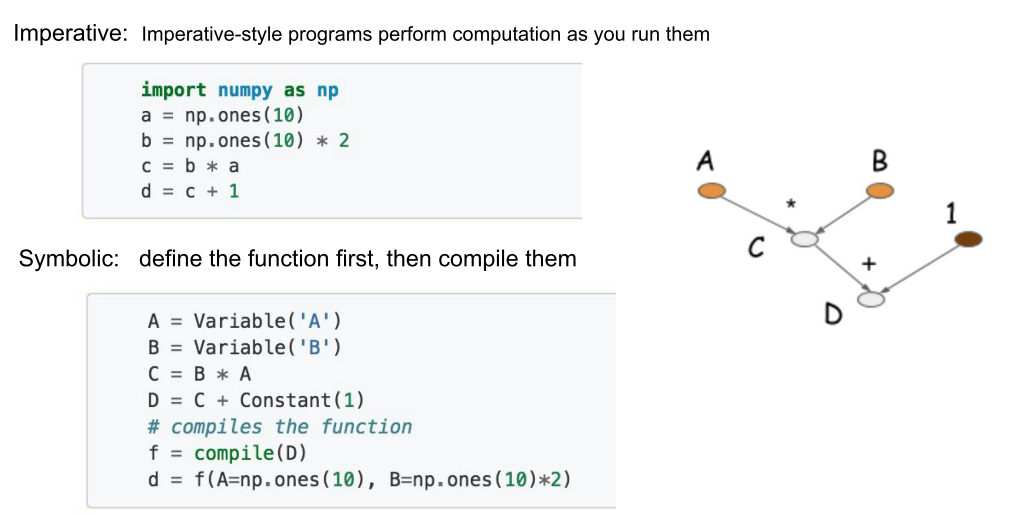
\includegraphics[width=0.9\linewidth,keepaspectratio]{pytorch1}
\end{center}

  {\tiny (Ref: Pytorch Tutorial - Chongruo Wu)}

\end{frame}

%%%%%%%%%%%%%%%%%%%%%%%%%%%%%%%%%%%%%%%%%%%%%%%%%%%
\begin{frame}[fragile] \frametitle{Popular Deep Learning Frameworks}


\begin{center}
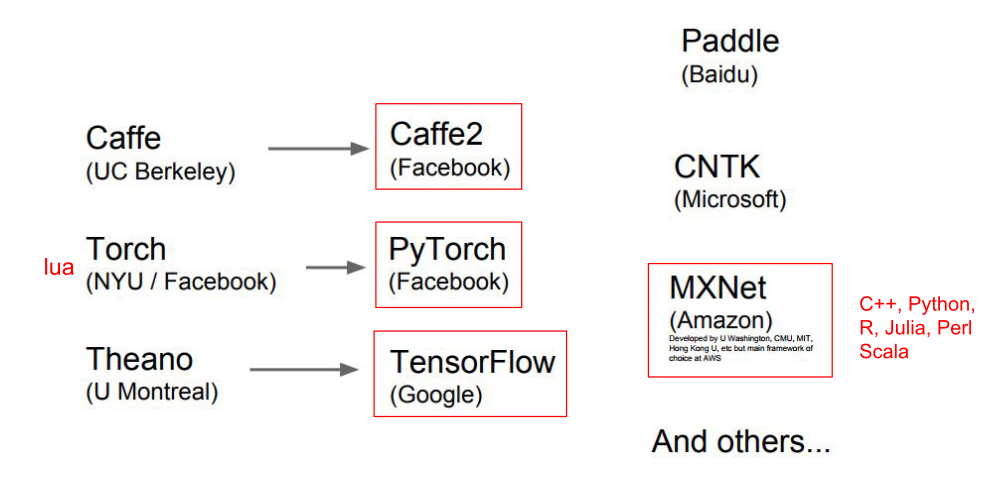
\includegraphics[width=0.9\linewidth,keepaspectratio]{pytorch2}
\end{center}

  {\tiny (Ref: Pytorch Tutorial - Chongruo Wu)}

\end{frame}



%%%%%%%%%%%%%%%%%%%%%%%%%%%%%%%%%%%%%%%%%%%%%%%%%%%
\begin{frame}[fragile] \frametitle{Installation}

Visit https://pytorch.org/get-started/locally/

\begin{center}
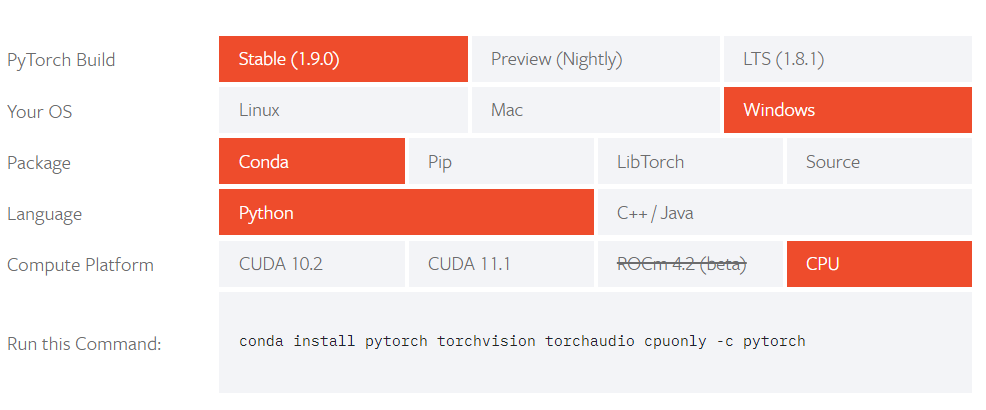
\includegraphics[width=\linewidth,keepaspectratio]{pyt39}%{pyt5}
\end{center}


\end{frame}


%%%%%%%%%%%%%%%%%%%%%%%%%%%%%%%%%%%%%%%%%%%%%%%%%%%
\begin{frame}[fragile] \frametitle{Imp Packages inside PyTorch}
\begin{itemize}
\item  torch: a Tensor library like Numpy, with strong GPU support
\item torch.autograd: an automatic differentiation library 
\item torch.nn: a neural networks library deeply integrated with autograd 
\item torch.optim: an optimization package to be used with torch.nn
\item torch.utils: DataLoader, Trainer and other utility functions for convenience
\end{itemize}
\end{frame}


%%%%%%%%%%%%%%%%%%%%%%%%%%%%%%%%%%%%%%%%%%%%%%%%%%%
\begin{frame}[fragile] \frametitle{Concepts of PyTorch}
\begin{itemize}
\item Data:
\begin{itemize}
\item Tensor
\item Variable (for Gradient)
\end{itemize}
\item Function:
\begin{itemize}
\item   NN Modules
\item   Optimizer
\item   Loss Function
\item   Multi-Processing
\end{itemize}
\end{itemize}
\end{frame}

 % %%%%%%%%%%%%%%%%%%%%%%%%%%%%%%%%%%%%%%%%%%%%%%%%%%%%%%%%%%%%%%%%%%%%%%%%%%%%%%%%%%
\begin{frame}[fragile]
\frametitle{What is a Tensor?}
\begin{itemize}
\item Tensors to encode the inputs and outputs of a model, as well as the model's parameters.
\item Similar to NumPy's ndarrays, except that tensors can run on GPUs or other hardware accelerators. (both actually share same underlying memory, if CPU)

\end{itemize}

 \begin{lstlisting}
import torch
import numpy as np

data = [[1, 2],[3, 4]]
x_data = torch.tensor(data)
x_data_numpy = x_data.numpy()

np_array = np.array(data)
x_np = torch.from_numpy(np_array)

 \end{lstlisting}
 
 
 \end{frame} 
 
 
 % %%%%%%%%%%%%%%%%%%%%%%%%%%%%%%%%%%%%%%%%%%%%%%%%%%%%%%%%%%%%%%%%%%%%%%%%%%%%%%%%%%
\begin{frame}[fragile]
\frametitle{What is a Tensor?}
\begin{itemize}
\item All of deep learning is computations on tensors
\item Array with dimension 0 is a scalar
\item Array with dimension 1 is a vector
\item Array with dimension 2 is a martix
\item Array with dimension 3 or more is a tensor
\item Tensors can be created from Python lists with the torch.tensor() function.
\end{itemize}
 \end{frame} 
 
 % %%%%%%%%%%%%%%%%%%%%%%%%%%%%%%%%%%%%%%%%%%%%%%%%%%%%%%%%%%%%%%%%%%%%%%%%%%%%%%%%%%
\begin{frame}[fragile]
\frametitle{1D Tensor}
1D Vector
 \begin{lstlisting}
 import torch

V_data = [1.,2.,3.]
V = torch.tensor(V_data)
print(V)

>>>tensor([ 1.,  2.,  3.])
 \end{lstlisting}

 \end{frame} 


 
%%%%%%%%%%%%%%%%%%%%%%%%%%%%%%%%%%%%%%%%%%%%%%%%%%%%%%%%%%%%%%%%%%%%%%%%%%%%%%%%%%
\begin{frame}[fragile]
\frametitle{2D Tensor}
Matrix 
 \begin{lstlisting}
M_data = [[1., 2., 3.], [4., 5., 6]]
M = torch.tensor(M_data)
print(M)

>>>tensor([[ 1.,  2.,  3.],
        [ 4.,  5.,  6.]])
 \end{lstlisting}

 \end{frame} 

 
 % %%%%%%%%%%%%%%%%%%%%%%%%%%%%%%%%%%%%%%%%%%%%%%%%%%%%%%%%%%%%%%%%%%%%%%%%%%%%%%%%%%
\begin{frame}[fragile]
\frametitle{3D Tensor}
3D tensor of size 2x2x2.
 \begin{lstlisting}
T_data = [[[1.,2.], [3.,4.]],
          [[5.,6.], [7.,8.]]]
T = torch.tensor(T_data)
print(T)


>>>tensor([[[ 1.,  2.],
         [ 3.,  4.]],

        [[ 5.,  6.],
         [ 7.,  8.]]])
 \end{lstlisting}

 \end{frame} 
 
  % %%%%%%%%%%%%%%%%%%%%%%%%%%%%%%%%%%%%%%%%%%%%%%%%%%%%%%%%%%%%%%%%%%%%%%%%%%%%%%%%%%
\begin{frame}[fragile]
\frametitle{Random, Constant Tensor}

\begin{lstlisting}
shape = (2,3,)
rand_tensor = torch.rand(shape)
ones_tensor = torch.ones(shape)
zeros_tensor = torch.zeros(shape)

print(f"Random Tensor: \n {rand_tensor} \n")
print(f"Ones Tensor: \n {ones_tensor} \n")
print(f"Zeros Tensor: \n {zeros_tensor}")

Random Tensor: 
 tensor([[0.5742, 0.4606, 0.0981],
        [0.3154, 0.0503, 0.0097]]) 

Ones Tensor: 
 tensor([[1., 1., 1.],
        [1., 1., 1.]]) 

Zeros Tensor: 
 tensor([[0., 0., 0.],
        [0., 0., 0.]])
 \end{lstlisting}

 \end{frame} 
 

 % %%%%%%%%%%%%%%%%%%%%%%%%%%%%%%%%%%%%%%%%%%%%%%%%%%%%%%%%%%%%%%%%%%%%%%%%%%%%%%%%%%
\begin{frame}[fragile]
\frametitle{Attributes of Tensor}

\begin{lstlisting}
tensor = torch.rand(3,4)

print(f"Shape of tensor: {tensor.shape}")
print(f"Datatype of tensor: {tensor.dtype}")
print(f"Device tensor is stored on: {tensor.device}")

Shape of tensor: torch.Size([3, 4])
Datatype of tensor: torch.float32
Device tensor is stored on: cpu
 \end{lstlisting}

 \end{frame} 
 
 
 % %%%%%%%%%%%%%%%%%%%%%%%%%%%%%%%%%%%%%%%%%%%%%%%%%%%%%%%%%%%%%%%%%%%%%%%%%%%%%%%%%%
\begin{frame}[fragile]
\frametitle{Indexing}
\begin{itemize}
\item Indexing into the vector gives you a scalar. 
\item Indexing into the matrix gives you a vector. 
\item Indexing into the tensor gives you a matrix!
\end{itemize}

 \begin{lstlisting}
print(V[0])
print(M[0])
print(T[0])

tensor(1.)
tensor([ 1.,  2.,  3.])
tensor([[ 1.,  2.],
        [ 3.,  4.]])
 \end{lstlisting}

 \end{frame} 
 
 
  % %%%%%%%%%%%%%%%%%%%%%%%%%%%%%%%%%%%%%%%%%%%%%%%%%%%%%%%%%%%%%%%%%%%%%%%%%%%%%%%%%%
\begin{frame}[fragile]
\frametitle{Data type}
\begin{itemize}
\item Default datatype in tensor is Float
\item For int tensor, call torch.LongTensor(), etc
\item To create a tensor with random data and the supplied dimensionality with torch.rand()
\end{itemize}

 \end{frame} 
 
%%%%%%%%%%%%%%%%%%%%%%%%%%%%%%%%%%%%%%%%%%%%%%%%%%%%%%%%%%%%%%%%%%%%%%%%%%%%%%%%%%
\begin{frame}[fragile]
\frametitle{Initialization}
 \begin{lstlisting}
x = torch.rand((3, 4, 5))
print(x)

>>>tensor([[[-1.5256, -0.7502, -0.6540, -1.6095, -0.1002],
         [-0.6092, -0.9798, -1.6091, -0.7121,  0.3037],
         [-0.7773, -0.2515, -0.2223,  1.6871,  0.2284],
         [ 0.4676, -0.6970, -1.1608,  0.6995,  0.1991]],

        [[ 0.8657,  0.2444, -0.6629,  0.8073,  1.1017],
         [-0.1759, -2.2456, -1.4465,  0.0612, -0.6177],
         [-0.7981, -0.1316,  1.8793, -0.0721,  0.1578],
         [-0.7735,  0.1991,  0.0457,  0.1530, -0.4757]],

        [[-0.1110,  0.2927, -0.1578, -0.0288,  0.4533],
         [ 1.1422,  0.2486, -1.7754, -0.0255, -1.0233],
         [-0.5962, -1.0055,  0.4285,  1.4761, -1.7869],
         [ 1.6103, -0.7040, -0.1853, -0.9962, -0.8313]]])
 \end{lstlisting}

 \end{frame} 
 
  % %%%%%%%%%%%%%%%%%%%%%%%%%%%%%%%%%%%%%%%%%%%%%%%%%%%%%%%%%%%%%%%%%%%%%%%%%%%%%%%%%%
\begin{frame}[fragile]
\frametitle{Operations on Tensors}
\begin{itemize}
\item 100s of operations available.
\item Each of these operations can be run on the GPU (at typically higher speeds than on a CPU).
\item By default, tensors are created on the CPU. 
\item Need to explicitly move tensors to the GPU using $.to$ method (after checking for GPU availability). 
\item Keep in mind that copying large tensors across devices can be expensive in terms of time and memory!
\end{itemize}

 \begin{lstlisting}
# We move our tensor to the GPU if available
if torch.cuda.is_available():
  tensor = tensor.to('cuda')
 \end{lstlisting}

 \end{frame} 
 
 
 
 %%%%%%%%%%%%%%%%%%%%%%%%%%%%%%%%%%%%%%%%%%%%%%%%%%%%%%%%%%%%%%%%%%%%%%%%%%%%%%%%%%
\begin{frame}[fragile]
\frametitle{Operations}
Operations with Tensors.

 Note:  In-place operations save some memory, but can be problematic when computing derivatives because of an immediate loss of history. Hence, their use is discouraged.
 
 
 \begin{lstlisting}
x = torch.tensor([1.,2.,3.])
y = torch.tensor([4.,5.,6.])
z = x + y
print(z)

>>>tensor([ 5.,  7.,  9.])

# Operations that store the result into the operand are called in-place. They are denoted by a _ suffix. For example: x.copy_(y), x.t_(), will change x.
 
tensor.add_(5)
\end{lstlisting}

\end{frame} 
 
 %%%%%%%%%%%%%%%%%%%%%%%%%%%%%%%%%%%%%%%%%%%%%%%%%%%%%%%%%%%%%%%%%%%%%%%%%%%%%%%%%%
\begin{frame}[fragile]
\frametitle{Operations}
Multiplication:

Many more mathematical operations are available.

\begin{lstlisting}
# This computes the matrix multiplication between two tensors. y1, y2, y3 will have the same value
y1 = tensor @ tensor.T
y2 = tensor.matmul(tensor.T)

y3 = torch.rand_like(tensor)
torch.matmul(tensor, tensor.T, out=y3)


# This computes the element-wise product. z1, z2, z3 will have the same value
z1 = tensor * tensor
z2 = tensor.mul(tensor)

z3 = torch.rand_like(tensor)
torch.mul(tensor, tensor, out=z3)
\end{lstlisting}
\end{frame} 
 
 
%%%%%%%%%%%%%%%%%%%%%%%%%%%%%%%%%%%%%%%%%%%%%%%%%%%%%%%%%%%%%%%%%%%%%%%%%%%%%%%%%%
\begin{frame}[fragile]
\frametitle{Concatenation}
Concatenation
 \begin{lstlisting}
# By default, it concatenates along the first axis (concatenates rows)
x_1 = torch.randn(2, 5)
y_1 = torch.randn(3, 5)
z_1 =torch.cat([x_1, y_1])
print(z_1)

# Concatenate columns:
x_2 = torch.randn(2, 3)
y_2 = torch.randn(2, 5)
z_2 = torch.cat([x_2, y_2], 1) # second arg specifies which axis to concat along
print(z_2)

# If your tensors are not compatible, torch will complain.  Uncomment to see the error
# torch.cat([x_1, x_2])
\end{lstlisting}
\end{frame} 
 
 %%%%%%%%%%%%%%%%%%%%%%%%%%%%%%%%%%%%%%%%%%%%%%%%%%%%%%%%%%%%%%%%%%%%%%%%%%%%%%%%%%
\begin{frame}[fragile]
\frametitle{Reshaping}
Reshaping Tensors with view() method.

If one of the dimensions is -1, its size can be inferred

\begin{lstlisting}
x = torch.randn(2,3,4)
print(x)
print(x.view(2,12)) # Reshape to 2 rows, 12 columns
print(x.view(2, -1)) # Same as above. 
\end{lstlisting}
\end{frame} 
 
%%%%%%%%%%%%%%%%%%%%%%%%%%%%%%%%%%%%%%%%%%%%%%%%%%%%%%%%%%%%%%%%%%%%%%%%%%%%%%%%%%
\begin{frame}[fragile]
\frametitle{Computation Graphs}

\begin{itemize}
\item It is a specification of how your data is combined to give you the output. 
\item Since the graph totally specifies what parameters were involved with which operations, it contains enough information to compute derivatives.
\end{itemize}
\end{frame} 

 
 %%%%%%%%%%%%%%%%%%%%%%%%%%%%%%%%%%%%%%%%%%%%%%%%%%%%%%%%%%%%%%%%%%%%%%%%%%%%%%%%%%
\begin{frame}[fragile]
\frametitle{Variables and Tensors}
\begin{itemize}
\item What does torch.tensor object has stored? : data and the shape, and maybe a few other things
\item But when we added two tensors together, we got an output tensor. 
\item All this output tensor knows is its data and shape. 
\item It has no idea that it was the sum of two other tensors (it could have been read in from a file, it could be the result of some other operation, etc.)
\item The Variable class keeps track of how it was created. 
\end{itemize}
Latest News: Variables and Tensors have merged!!!
\end{frame} 
 
 
%%%%%%%%%%%%%%%%%%%%%%%%%%%%%%%%%%%%%%%%%%%%%%%%%%%%%%%%%%%%%%%%%%%%%%%%%%%%%%%%%%
\begin{frame}[fragile]
\frametitle{PyTorch 0.4.0 release notes}
\begin{itemize}
\item Tensors and Variables have merged
\item torch.autograd.Variable and torch.tensor are now the same class. 
\item More precisely, torch.tensor is capable of tracking history and behaves like the old Variable; Variable wrapping continues to work as before but returns an object of type torch.tensor. \item No need the Variable wrapper everywhere in your code anymore.
\end{itemize}
 \begin{lstlisting}
>>> x = torch.DoubleTensor([1, 1, 1])
>>> print(type(x)) # was torch.DoubleTensor
<class 'torch.autograd.variable.Variable'>
>>> print(x.type())  # OK: 'torch.DoubleTensor'
'torch.DoubleTensor'
>>> print(isinstance(x, torch.DoubleTensor))  # OK: True
True
\end{lstlisting}
\end{frame} 
 
    %%%%%%%%%%%%%%%%%%%%%%%%%%%%%%%%%%%%%%%%%%%%%%%%%%%%%%%%%%%%%%%%%%%%%%%%%%%%%%%%%%
\begin{frame}[fragile]
\frametitle{PyTorch 0.4.0 release notes}

\begin{itemize}
\item When does autograd start tracking history now?
\item requires\_grad, the central flag for autograd, is now an attribute on Tensors.
\end{itemize}
 \begin{lstlisting}
>>> x = torch.ones(1)  # create a tensor with requires_grad=False (default)
>>> x.requires_grad
False
>>> y = torch.ones(1)  # another tensor with requires_grad=False
>>> z = x + y
>>> # both inputs have requires_grad=False. so does the output
>>> z.requires_grad
False
>>> # then autograd won't track this computation. let's verify!
>>> z.backward()
RuntimeError: element 0 of tensors does not require grad and does not have a grad_fn
\end{lstlisting}
\end{frame} 
 
     %%%%%%%%%%%%%%%%%%%%%%%%%%%%%%%%%%%%%%%%%%%%%%%%%%%%%%%%%%%%%%%%%%%%%%%%%%%%%%%%%%
\begin{frame}[fragile]
\frametitle{PyTorch 0.4.0 release notes}

 \begin{lstlisting}
>>>
>>> # now create a tensor with requires_grad=True
>>> w = torch.ones(1, requires_grad=True)
>>> w.requires_grad
True
>>> # add to the previous result that has require_grad=False
>>> total = w + z
>>> # the total sum now requires grad!
>>> total.requires_grad
True
>>> # autograd can compute the gradients as well
>>> total.backward()
>>> w.grad
tensor([ 1.])
>>> # and no computation is wasted to compute gradients for x, y and z, which don't require grad
>>> z.grad == x.grad == y.grad == None
True
\end{lstlisting}
\end{frame} 
 
     %%%%%%%%%%%%%%%%%%%%%%%%%%%%%%%%%%%%%%%%%%%%%%%%%%%%%%%%%%%%%%%%%%%%%%%%%%%%%%%%%%
\begin{frame}[fragile]
\frametitle{PyTorch 0.4.0 release notes}

\begin{itemize}
\item What about .data?
\item .data was the primary way to get the underlying Tensor from a Variable. 
\item After this merge, calling y = x.data still has similar semantics.
\item So y will be a Tensor that shares the same data with x, is unrelated with the computation history of x, and has requires\_grad=False.
\end{itemize}

From now onwards, even if Variables and Tensors are mentioned disticnlty, from 0.4.0, they are just the Tensors with grad\_fn available.
\end{frame} 
 
 
  
  %%%%%%%%%%%%%%%%%%%%%%%%%%%%%%%%%%%%%%%%%%%%%%%%%%%%%%%%%%%%%%%%%%%%%%%%%%%%%%%%%%
\begin{frame}[fragile]
\frametitle{Tensor/Variables operations}

So now, what is the derivative of this sum with respect to the first component of x? 


 \begin{lstlisting}
x = torch.tensor([1.,2.,3.])
y = torch.tensor([4.,5.,6.])
x.requires_grad = True
y.requires_grad = True
z = x + y
print(z.data)
>>>tensor([ 5.,  7.,  9.])
print(z.grad_fn)
>>><AddBackward1 object at 0x000000000A9C94A8>
s = z.sum()
print(s.data)
>>>tensor(21.)
print(s.grad_fn)
>>><SumBackward0 object at 0x000000000A9C94E0>
\end{lstlisting}
\end{frame} 
 
%%%%%%%%%%%%%%%%%%%%%%%%%%%%%%%%%%%%%%%%%%%%%%%%%%%%%%%%%%%%%%%%%%%%%%%%%%%%%%%%%%
\begin{frame}[fragile]
\frametitle{Derivative}
\begin{itemize}
\item Need $\frac{\partial s}{\partial x_0}$
\item s knows that it was created as a sum of the tensor z. 
\item z knows that it was the sum x + y. 
\item So, $s = \overbrace{x_0 + y_0}^\text{$z_0$} + \overbrace{x_1 + y_1}^\text{$z_1$} + \overbrace{x_2 + y_2}^\text{$z_2$}$
\item Enough information to determine that the derivative : Pytorch knows how to compute their gradients of sum() and + operations, and run the back propagation algorithm. 
\end{itemize}


\end{frame} 
 
 %%%%%%%%%%%%%%%%%%%%%%%%%%%%%%%%%%%%%%%%%%%%%%%%%%%%%%%%%%%%%%%%%%%%%%%%%%%%%%%%%%
\begin{frame}[fragile]
\frametitle{Back Propagation}

\begin{lstlisting}
s.backward() # calling .backward() on any variable will run backprop, starting from it.
print(x.grad)

>>>tensor([ 1.,  1.,  1.])
\end{lstlisting}

\end{frame} 
 
 
  %%%%%%%%%%%%%%%%%%%%%%%%%%%%%%%%%%%%%%%%%%%%%%%%%%%%%%%%%%%%%%%%%%%%%%%%%%%%%%%%%%
\begin{frame}[fragile]
\frametitle{Variable Gradient}
Note:
 \begin{lstlisting}
x = torch.randn((2,2))
y = torch.randn((2,2))
x.requires_grad = True
y.requires_grad = True
z = x + y 
print(z.grad_fn)
>>><AddBackward1 object at 0x000000000A9D2358>

var_z_data = z.data # Get the wrapped Tensor object out of var_z...
new_var_z = torch.tensor( var_z_data ) # Re-wrap the tensor in a new variable

# does new_var_z have info to backprop to x and y? NO!
print(new_var_z.grad_fn)
>>>None
# And how could it?  We copied the tensor values out of z (that is what z.data is).  This tensor doesn't know anything about how it was computed.   If var_z_data doesn't know how it was computed, theres no way new_var_z will.
\end{lstlisting}

\end{frame} 
 

%%%%%%%%%%%%%%%%%%%%%%%%%%%%%%%%%%%%%%%%%%%%%%%%%%%
\begin{frame}[fragile] \frametitle{Autograd: automatic gradient}
\begin{itemize}
\item Provides automatic differentiation for all operations on Tensors
\item It is a define-by-run framework, which means that your backprop is defined by how your code is run, and that every single iteration can be different.
\end{itemize}
\end{frame}

%%%%%%%%%%%%%%%%%%%%%%%%%%%%%%%%%%%%%%%%%%%%%%%%%%%
\begin{frame}[fragile] \frametitle{Automatic differentiation}

\begin{itemize}
\item In $backpropogation$ parameters (model weights) are adjusted according to the gradient of the loss function with respect to the given parameter.
\item To compute those gradients, PyTorch has a built-in differentiation engine called \lstinline|torch.autograd|. 
\item It supports automatic computation of gradient for any computational graph.
\item Consider the simplest one-layer neural network, with input x, parameters w and b, and some loss function.
\end{itemize}

\tiny{(Ref: Microsoft - Intro to Machine Learning using Pytorch)}


\begin{lstlisting}
import torch

x = torch.ones(5)  # input tensor
y = torch.zeros(3)  # expected output
w = torch.randn(5, 3, requires_grad=True)
b = torch.randn(3, requires_grad=True)
z = torch.matmul(x, w)+b
loss = torch.nn.functional.binary_cross_entropy_with_logits(z, y)
\end{lstlisting}

\end{frame}

%%%%%%%%%%%%%%%%%%%%%%%%%%%%%%%%%%%%%%%%%%%%%%%%%%%
\begin{frame}[fragile] \frametitle{Tensors, Functions and Computational graph}

\begin{center}
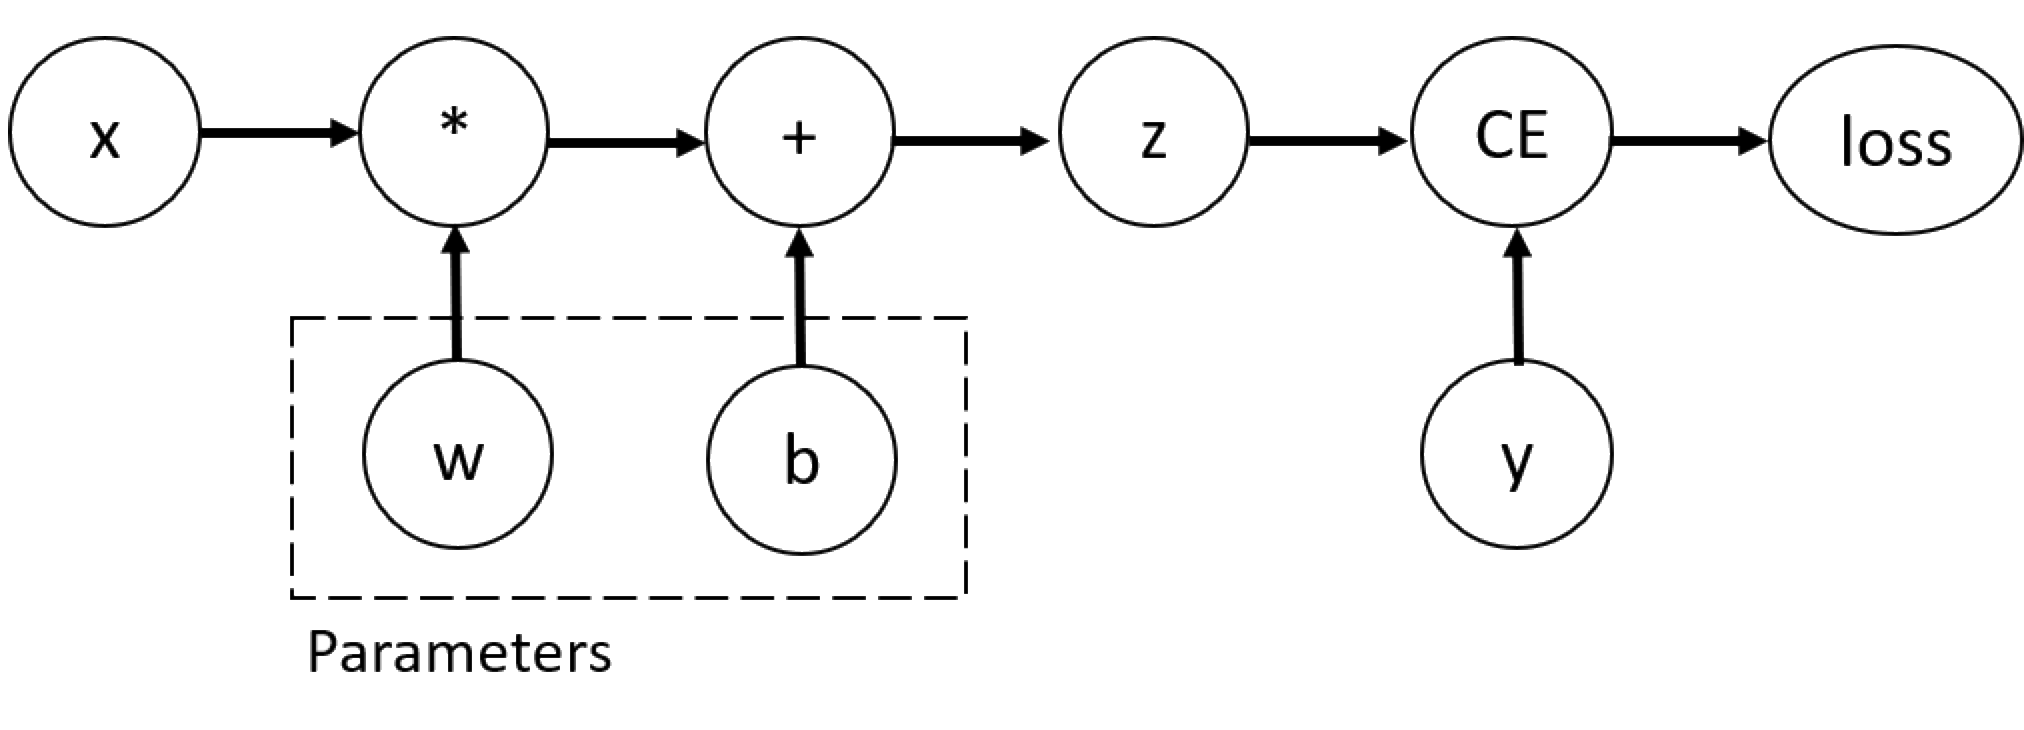
\includegraphics[width=\linewidth,keepaspectratio]{pyt40}
\end{center}

\begin{itemize}
\item In this network, w and b are parameters, which need to be optimized. 
\item Need to be able to compute the gradients of loss function with respect to those variables. 
\item Set the \lstinline|requires_grad| property of those tensors. Note: You can set the value of \lstinline|requires_grad| when creating a tensor, or later by using \lstinline|x.requires_grad_(True)| method.
\end{itemize}


\tiny{(Ref: Microsoft - Intro to Machine Learning using Pytorch)}
\end{frame}

%%%%%%%%%%%%%%%%%%%%%%%%%%%%%%%%%%%%%%%%%%%%%%%%%%%
\begin{frame}[fragile] \frametitle{Tensors, Functions and Computational graph}


\begin{itemize}
\item A function that we apply to tensors to construct computational graph is in fact an object of class Function. 
\item This object knows how to compute the function in the forward direction, and also how to compute its derivative during the backward propagation step. 
\item A reference to the backward propagation function is stored in \lstinline|grad_fn| property of a tensor.
\end{itemize}

\tiny{(Ref: Microsoft - Intro to Machine Learning using Pytorch)}


\begin{lstlisting}
print('Gradient function for z =',z.grad_fn)
print('Gradient function for loss =', loss.grad_fn)

>>>Gradient function for z = <AddBackward0 object at 0x7fcaa4928110>
Gradient function for loss = <BinaryCrossEntropyWithLogitsBackward object at 0x7fcaa4928250>
\end{lstlisting}

\end{frame}

%%%%%%%%%%%%%%%%%%%%%%%%%%%%%%%%%%%%%%%%%%%%%%%%%%%
\begin{frame}[fragile] \frametitle{Computing gradients}

\begin{itemize}
\item To optimize weights of parameters in the neural network, we need to compute the derivatives of our loss function with respect to parameters, namely, we need  $\frac{\partial loss}{\partial w}$ and
$\frac{\partial loss}{\partial b}$   under some fixed values of x and y. 
\item To compute those derivatives, we call \lstinline|loss.backward()|, and then retrieve the values from \lstinline|w.grad| and \lstinline|b.grad|:
\end{itemize}

\tiny{(Ref: Microsoft - Intro to Machine Learning using Pytorch)}


\begin{lstlisting}
loss.backward()
print(w.grad)
print(b.grad)

>>>tensor([[0.2739, 0.0490, 0.3279],
        [0.2739, 0.0490, 0.3279],
        [0.2739, 0.0490, 0.3279],
        [0.2739, 0.0490, 0.3279],
        [0.2739, 0.0490, 0.3279]])
tensor([0.2739, 0.0490, 0.3279])
\end{lstlisting}

\end{frame}

%%%%%%%%%%%%%%%%%%%%%%%%%%%%%%%%%%%%%%%%%%%%%%%%%%%
\begin{frame}[fragile] \frametitle{Computing gradients}

Note:
\begin{itemize}
\item We can only obtain the grad properties for the leaf nodes of the computational graph, which have \lstinline|requires_grad| property set to True. 
\item For all other nodes in our graph, gradients will not be available. 
\item In addition, we can only perform gradient calculations using backward once on a given graph, for performance reasons. 
\item If we need to do several backward calls on the same graph, we need to pass \lstinline|retain_graph=True| to the backward call.
\item By default, all tensors with \lstinline|requires_grad=True| are tracking their computational history and support gradient computation. 
\item However, if we only want to do forward computations through the network. We can stop tracking computations by surrounding our computation code with \lstinline|torch.no_grad()| block.
\item Disabling can also be used to mark some parameters in your neural network at frozen parameters, say, for pre-trained networks.
\end{itemize}

\tiny{(Ref: Microsoft - Intro to Machine Learning using Pytorch)}



\end{frame}

%%%%%%%%%%%%%%%%%%%%%%%%%%%%%%%%%%%%%%%%%%%%%%%%%%%
\begin{frame}[fragile] \frametitle{Computing gradients}

\tiny{(Ref: Microsoft - Intro to Machine Learning using Pytorch)}


\begin{lstlisting}
z = torch.matmul(x, w)+b
print(z.requires_grad)

with torch.no_grad():
    z = torch.matmul(x, w)+b
print(z.requires_grad)

>>>True
False
\end{lstlisting}

\end{frame}


%%%%%%%%%%%%%%%%%%%%%%%%%%%%%%%%%%%%%%%%%%%%%%%%%%%
\begin{frame}[fragile] \frametitle{Computational Graphs}


\begin{itemize}
\item Conceptually, autograd keeps a record of data (tensors) and all executed operations (along with the resulting new tensors) in a directed acyclic graph (DAG) consisting of Function objects. 
\item In this DAG, leaves are the input tensors, roots are the output tensors. 
\item By tracing this graph from roots to leaves, you can automatically compute the gradients using the chain rule.
\item In a forward pass, autograd does two things simultaneously:
	\begin{itemize}
	\item run the requested operation to compute a resulting tensor
	\item maintain the operation’s gradient function in the DAG.
	\end{itemize}
\item The backward pass kicks off when .backward() is called on the DAG root. autograd then:
	\begin{itemize}
	\item computes the gradients from each \lstinline|.grad_fn|,
	\item accumulates them in the respective tensor’s \lstinline|.grad| attribute
	\item using the chain rule, propagates all the way to the leaf tensors.
	\end{itemize}

\end{itemize}


\tiny{(Ref: Microsoft - Intro to Machine Learning using Pytorch)}
\end{frame}

%%%%%%%%%%%%%%%%%%%%%%%%%%%%%%%%%%%%%%%%%%%%%%%%%%%
\begin{frame}[fragile] \frametitle{Computional Graphs}
DAGs are dynamic in PyTorch

\begin{itemize}
\item The graph is recreated from scratch; after each \lstinline|.backward()| call, autograd starts populating a new graph. 
\item This is exactly what allows you to use control flow statements in your model; you can change the shape, size and operations at every iteration if needed.
\end{itemize}


\tiny{(Ref: Microsoft - Intro to Machine Learning using Pytorch)}
\end{frame}

%%%%%%%%%%%%%%%%%%%%%%%%%%%%%%%%%%%%%%%%%%%%%%%%%%%
\begin{frame}[fragile] \frametitle{Computional Graphs}
Odd cases
\begin{itemize}
\item In case of a scalar loss function, and we need to compute the gradient with respect to some parameters. 
\item However, there are cases when the output function is an arbitrary tensor. 
\item In this case, PyTorch allows you to compute so-called Jacobian product, and not the actual gradient.
\item For a vector function $\vec{y}=f(\vec{x})$, where
$\vec{x}=\langle x_1,\dots,x_n\rangle$ and
$\vec{y}=\langle y_1,\dots,y_m\rangle$, a gradient of
$\vec{y}$ with respect to $\vec{x}$ is given by \lstinline|Jacobian matrix|

% \begin{align}
% \begin{align}J=\left(\begin{array}{ccc}
      % \frac{\partial y_{1}}{\partial x_{1}} & \cdots & \frac{\partial y_{1}}{\partial x_{n}}\\
      % \vdots & \ddots & \vdots\\
      % \frac{\partial y_{m}}{\partial x_{1}} & \cdots & \frac{\partial y_{m}}{\partial x_{n}}
      % \end{array}\right)
% \end{align}
% \end{align}

\item Instead of computing the Jacobian matrix itself, PyTorch allows you to
compute **Jacobian Product** $v^T\cdot J$ for a given input vector
$v=(v_1 \dots v_m)$. This is achieved by calling `backward` with
$v$ as an argument. The size of $v$ should be the same as
the size of the original tensor, with respect to which we want to
compute the product
\end{itemize}


\tiny{(Ref: Microsoft - Intro to Machine Learning using Pytorch)}
\end{frame}


%%%%%%%%%%%%%%%%%%%%%%%%%%%%%%%%%%%%%%%%%%%%%%%%%%%
\begin{frame}[fragile] \frametitle{Computational Graphs}

\begin{itemize}
\item Notice that when we call backward for the second time with the same argument, the value of the gradient is different. 
\item This happens because PyTorch accumulates the gradients, i.e. the value of computed gradients is added to the grad property of all leaf nodes of computational graph. 
\item If you want to compute the proper gradients, you need to zero out the grad property before. 
\item \lstinline|backward()| is equivalent to calling \lstinline|backward(torch.tensor(1.0))|, which is a useful way to compute the gradients in case of a scalar-valued function, such as loss during neural network training.
\end{itemize}


\tiny{(Ref: Microsoft - Intro to Machine Learning using Pytorch)}




\end{frame}

%%%%%%%%%%%%%%%%%%%%%%%%%%%%%%%%%%%%%%%%%%%%%%%%%%%
\begin{frame}[fragile] \frametitle{Computational Graphs}


\tiny{(Ref: Microsoft - Intro to Machine Learning using Pytorch)}

\begin{lstlisting}
inp = torch.eye(5, requires_grad=True)
out = (inp+1).pow(2)
out.backward(torch.ones_like(inp), retain_graph=True)
print("First call\n", inp.grad)
out.backward(torch.ones_like(inp), retain_graph=True)
print("\nSecond call\n", inp.grad)
inp.grad.zero_()
out.backward(torch.ones_like(inp), retain_graph=True)
print("\nCall after zeroing gradients\n", inp.grad)

\end{lstlisting}


\end{frame}

% %%%%%%%%%%%%%%%%%%%%%%%%%%%%%%%%%%%%%%%%%%%%%%%%%%%
% \begin{frame}[fragile] \frametitle{Function}
% \begin{itemize}
% \item Implements forward and backward definitions of an autograd operation. 
% \item Every Variable operation, creates at least a single Function node, that connects to functions that created a Variable and encodes its history.
% \item Variable and Function are interconnected and build up an acyclic graph, that encodes a complete history of computation.
% \item Each variable has a .grad\_fn attribute that references a Function that has created the Variable (except for Variables created by the user - their grad\_fn is None).
% \end{itemize}
% \end{frame}

%%%%%%%%%%%%%%%%%%%%%%%%%%%%%%%%%%%%%%%%%%%%%%%%%%%%%%%%%%%%%%%%%%%%%%%%%%%%%%%%%%
\begin{frame}[fragile]
\frametitle{Activation Functions}

\begin{itemize}
\item Neural network consists of composing linearities with non-linearities, a long chains of affine compositions.
\item Non-linearities like $\tanh(x), \sigma(x), \text{ReLU}(x)$ are the most common.
\item Why these functions? I can think of plenty of other non-linearities.
\end{itemize}
\end{frame} 

%%%%%%%%%%%%%%%%%%%%%%%%%%%%%%%%%%%%%%%%%%%%%%%%%%%%%%%%%%%%%%%%%%%%%%%%%%%%%%%%%%
\begin{frame}[fragile]
\frametitle{Activation}

\begin{itemize}
\item The reason for this is that they have gradients that are easy to compute, and computing gradients is essential for learning. For example $ \frac{d\sigma}{dx} = \sigma(x)(1 - \sigma(x)) $
\item $ \sigma(x)$ less popular because the gradient vanishes very quickly as the absolute value of the argument grows. Small gradients means it is hard to learn. Most use tanh or ReLU.
\end{itemize}

 Note, all negatives are made 0 and positives kept as they are.

\begin{lstlisting}
data = torch.randn(2,2,requires_grad=True)
print(data)
import torch.nn.functional as F
print(F.relu(data))
>>>tensor([[ 1.6169, -0.9026],
			[ 0.1737,  0.0772]])
tensor([[ 1.6169,  0.0000],
			[ 0.1737,  0.0772]])
\end{lstlisting}
\end{frame} 

%%%%%%%%%%%%%%%%%%%%%%%%%%%%%%%%%%%%%%%%%%%%%%%%%%%%%%%%%%%%%%%%%%%%%%%%%%%%%%%%%%
\begin{frame}[fragile]
\frametitle{Softmax and Probabilities}

It should be clear that the output is a probability distribution: each element is non-negative and the sum over all components is 1.

\begin{itemize}
\item The function $\text{Softmax}(x)$ is also just a non-linearity, but it is special in that it usually is the last operation done in a network. 
\item This is because it takes in a vector of real numbers and returns a probability distribution.
\end{itemize}
 \begin{lstlisting}
data = torch.randn(5,requires_grad=True)
print(data)
print(F.softmax(data,0))
print(F.softmax(data,0).sum())

>>>tensor([ 0.1896, -0.2204,  0.1491,  0.0100, -0.1243])
tensor([ 0.2387,  0.1584,  0.2292,  0.1994,  0.1744])
tensor(1.)
 \end{lstlisting}

\end{frame} 

%%%%%%%%%%%%%%%%%%%%%%%%%%%%%%%%%%%%%%%%%%%%%%%%%%%%%%%%%%%%%%%%%%%%%%%%%%%%%%%%%%
\begin{frame}[fragile]
\frametitle{Objective or Loss or Cost function}

\begin{itemize}
\item Neural network is being trained to minimize it.
\item The parameters of the model are then updated by taking the derivative of the loss function. 
\item An example loss function is the negative log likelihood loss, which is a very common objective for multi-class classification.
\item We can compute gradients with respect to all of the parameters used to compute it! Then we can perform standard gradient updates.
\item Let $\theta$ be our parameters,  $L(\theta)$ the loss function, and $\eta$ a positive learning rate. Then:

$$ \theta^{(t+1)} = \theta^{(t)} - \eta \nabla_\theta L(\theta) $$
\end{itemize}

\end{frame} 

%%%%%%%%%%%%%%%%%%%%%%%%%%%%%%%%%%%%%%%%%%%%%%%%%%%%%%%%%%%%%%%%%%%%%%%%%%%%%%%%%%
\begin{frame}[fragile]
\frametitle{Optimization}

\begin{itemize}
\item Training a model is an iterative process; in each iteration (called an epoch) the model makes a guess about the output, calculates the error in its guess (loss), collects the derivatives of the error with respect to its parameters (as we saw in the module), and optimizes these parameters using gradient descent.
\item Many optimization methods do something more than just this vanilla gradient update.
\item Many attempt to vary the learning rate based on what is happening at train time. 
\item Torch provies many in the torch.optim package, and they are all completely transparent. 
\item Using the simplest gradient update is the same as the more complicated algorithms. 
\item Trying different algorithms and different parameters 
\item Other choices: Adam or RMSProp will boost performance noticably.
\end{itemize}

\end{frame} 

%%%%%%%%%%%%%%%%%%%%%%%%%%%%%%%%%%%%%%%%%%%%%%%%%%%
\begin{frame}[fragile] \frametitle{Setting hyperparameters}

Hyperparameters are adjustable parameters that let you control the model optimization process. Example:

\begin{itemize}
\item Number of Epochs: the number times to iterate over the dataset
\item Batch Size: the number of data samples seen by the model in each epoch
\item Learning Rate : how much to update models parameters at each batch/epoch. Smaller values yield slow learning speed, while large values may result in unpredictable behavior during training.
\end{itemize}




Each epoch consists of two main parts:

\begin{itemize}
\item The Train Loop: iterate over the training dataset and try to converge to optimal parameters.
\item The Validation/Test Loop: iterate over the test dataset to check if model performance is improving.
\end{itemize}

\tiny{(Ref: Microsoft - Intro to Machine Learning using Pytorch)}

\begin{lstlisting}
learning_rate = 1e-3
batch_size = 64
epochs = 5
\end{lstlisting}
\end{frame}


%%%%%%%%%%%%%%%%%%%%%%%%%%%%%%%%%%%%%%%%%%%%%%%%%%%
\begin{frame}[fragile] \frametitle{Loss}


\begin{itemize}
\item Loss function measures the degree of dissimilarity of obtained result to the target value, and it is the loss function that we want to minimize during training. \item To calculate the loss we make a prediction using the inputs of our given data sample and compare it against the true data label value.
\item Common loss functions include \lstinline|nn.MSELoss| (Mean Square Error) for regression tasks, and \lstinline|nn.NLLLoss| (Negative Log Likelihood) for classification. 
\item \lstinline|nn.CrossEntropyLoss| combines \lstinline|nn.LogSoftmax| and \lstinline|nn.NLLLoss|.
\end{itemize}

\tiny{(Ref: Microsoft - Intro to Machine Learning using Pytorch)}

\begin{lstlisting}
# Initialize the loss function
loss_fn = nn.CrossEntropyLoss()
\end{lstlisting}

\end{frame}

%%%%%%%%%%%%%%%%%%%%%%%%%%%%%%%%%%%%%%%%%%%%%%%%%%%
\begin{frame}[fragile] \frametitle{Optimization pass}


\begin{itemize}
\item Optimization is the process of adjusting model parameters to reduce model error in each training step. 
\item Optimization algorithms define how this process is performed (in this example we use Stochastic Gradient Descent). 
\item All optimization logic is encapsulated in the optimizer object. Here, we use the SGD optimizer; additionally, there are many different optimizers available in PyTorch such as ADAM and RMSProp, that work better for different kinds of models and data.
\item We initialize the optimizer by registering the model's parameters that need to be trained, and passing in the learning rate hyperparameter.
\end{itemize}

\tiny{(Ref: Microsoft - Intro to Machine Learning using Pytorch)}


\begin{lstlisting}
optimizer = torch.optim.SGD(model.parameters(), lr=learning_rate)
\end{lstlisting}

\end{frame}

%%%%%%%%%%%%%%%%%%%%%%%%%%%%%%%%%%%%%%%%%%%%%%%%%%%
\begin{frame}[fragile] \frametitle{Optimization Pass}

Inside the training loop, optimization happens in three steps:

\begin{itemize}
\item Call \lstinline|optimizer.zero_grad()| to reset the gradients of model parameters. Gradients by default add up; to prevent double-counting, we explicitly zero them at each iteration.
\item Back-propagate the prediction loss with a call to \lstinline|loss.backwards()|. PyTorch deposits the gradients of the loss w.r.t. each parameter.
\item Once we have our gradients, we call \lstinline|optimizer.step()| to adjust the parameters by the gradients collected in the backward pass.
\item We initialize the loss function and optimizer, and pass it to \lstinline|train_loop| and \lstinline|test_loop|.
\end{itemize}


\tiny{(Ref: Microsoft - Intro to Machine Learning using Pytorch)}
\end{frame}

%%%%%%%%%%%%%%%%%%%%%%%%%%%%%%%%%%%%%%%%%%%%%%%%%%%
\begin{frame}[fragile] \frametitle{Training Loop}

\tiny{(Ref: Microsoft - Intro to Machine Learning using Pytorch)}

\begin{lstlisting}
def train_loop(dataloader, model, loss_fn, optimizer):
    size = len(dataloader.dataset)
    for batch, (X, y) in enumerate(dataloader):        
        # Compute prediction and loss
        pred = model(X)
        loss = loss_fn(pred, y)
        
        # Backpropagation
        optimizer.zero_grad()
        loss.backward()
        optimizer.step()

        if batch % 100 == 0:
            loss, current = loss.item(), batch * len(X)
            print(f"loss: {loss:>7f}  [{current:>5d}/{size:>5d}]")
\end{lstlisting}

\end{frame}




%%%%%%%%%%%%%%%%%%%%%%%%%%%%%%%%%%%%%%%%%%%%%%%%%%%
\begin{frame}[fragile] \frametitle{Testing Loop}

\tiny{(Ref: Microsoft - Intro to Machine Learning using Pytorch)}

\begin{lstlisting}
def test_loop(dataloader, model, loss_fn):
    size = len(dataloader.dataset)
    test_loss, correct = 0, 0

    with torch.no_grad():
        for X, y in dataloader:
            pred = model(X)
            test_loss += loss_fn(pred, y).item()
            correct += (pred.argmax(1) == y).type(torch.float).sum().item()
            
    test_loss /= size
    correct /= size
    print(f"Test Error: \n Accuracy: {(100*correct):>0.1f}%, Avg loss: {test_loss:>8f} \n")
\end{lstlisting}

\end{frame}


%%%%%%%%%%%%%%%%%%%%%%%%%%%%%%%%%%%%%%%%%%%%%%%%%%%
\begin{frame}[fragile] \frametitle{Iterations}

\tiny{(Ref: Microsoft - Intro to Machine Learning using Pytorch)}


\begin{lstlisting}
loss_fn = nn.CrossEntropyLoss()
optimizer = torch.optim.SGD(model.parameters(), lr=learning_rate)

epochs = 10
for t in range(epochs):
    print(f"Epoch {t+1}\n-------------------------------")
    train_loop(train_dataloader, model, loss_fn, optimizer)
    test_loop(test_dataloader, model, loss_fn)
print("Done!")
\end{lstlisting}

\end{frame}



%%%%%%%%%%%%%%%%%%%%%%%%%%%%%%%%%%%%%%%%%%%%%%%%%%%
\begin{frame}[fragile] \frametitle{Save and load the model}

\lstinline|torch.save| persists \lstinline|state_dict| which is an internal state dictionary storing the learned parameters.

Note: Be sure to call model.eval() method before inferencing to set the dropout and batch normalization layers to evaluation mode. Failing to do this will yield inconsistent inference results.

\tiny{(Ref: Microsoft - Intro to Machine Learning using Pytorch)}

\begin{lstlisting}
model = models.vgg16(pretrained=True)
torch.save(model.state_dict(), 'data/model_weights.pth')

# load_state_dict() load the parameters 

model = models.vgg16() # we do not specify pretrained=True, i.e. do not load default weights
model.load_state_dict(torch.load('data/model_weights.pth'))
model.eval()
\end{lstlisting}


\end{frame}


%%%%%%%%%%%%%%%%%%%%%%%%%%%%%%%%%%%%%%%%%%%%%%%%%%%
\begin{frame}[fragile] \frametitle{Save and load the model}

If we want to store the architecture also, along with weights then pass the whole model to \lstinline|torch.save|

Note: This approach uses Python pickle module when serializing the model, thus it relies on the actual class definition to be available when loading the model.

\tiny{(Ref: Microsoft - Intro to Machine Learning using Pytorch)}

\begin{lstlisting}
torch.save(model, 'data/vgg_model.pth')

# We can then load the model like this:

model = torch.load('data/vgg_model.pth')
\end{lstlisting}


\end{frame}

%%%%%%%%%%%%%%%%%%%%%%%%%%%%%%%%%%%%%%%%%%%%%%%%%%%
\begin{frame}[fragile] \frametitle{ONNX}

\begin{itemize}
\item PyTorch also has native ONNX export support. 
\item Given the dynamic nature of the PyTorch execution graph, however, the export process must traverse the execution graph to produce a persisted ONNX model. 
\item For this reason, a test variable of the appropriate size should be passed in to the export routine (in our case, we will create a dummy zero tensor of the correct size):
\end{itemize}

There are a lot of things you can do with ONNX model, including running inference on different platforms and in different programming languages. 

\tiny{(Ref: Microsoft - Intro to Machine Learning using Pytorch)}

\begin{lstlisting}
input_image = torch.zeros((1,3,224,224))
onnx.export(model, input_image, 'data/model.onnx')
\end{lstlisting}


\end{frame}


% %%%%%%%%%%%%%%%%%%%%%%%%%%%%%%%%%%%%%%%%%%%%%%%%%%%%%%%%%%%%%%%%%%%%%%%%%%%%%%%%%%
% \begin{frame}[fragile]
% \frametitle{Neural Network Architecture}

% \begin{itemize}
% \item Should inherit from nn.Module and override the forward() method.
% \item  nn.Module makes it keep track of its trainable parameters, you can swap it between CPU and GPU with the .cuda() or .cpu() functions, etc.
% \end{itemize}

% \end{frame} 



% %%%%%%%%%%%%%%%%%%%%%%%%%%%%%%%%%%%%%%%%%%%%%%%%%%%
% \begin{frame}[fragile] \frametitle{Fundamental Data Types}
% Tensors: Similar to numpy ndarry but leverage GPU
% \begin{lstlisting}
% import torch

% x = torch.tensor(5, 3)
% print(x)

% 0.0000   0.0000   0.0001
  % 0.0000   0.0001   0.0000
  % 3.3717   0.0000   3.3717
  % 0.0000   3.8859   0.0000
  % 3.8001   0.0000  27.0173
% [torch.FloatTensor of size 5x3]
% \end{lstlisting}
% \end{frame}

% %%%%%%%%%%%%%%%%%%%%%%%%%%%%%%%%%%%%%%%%%%%%%%%%%%%
% \begin{frame}[fragile] \frametitle{Fundamental Data Types}
% Construct a randomly initialized matrix
% \begin{lstlisting}
% import torch

% x = torch.rand(5, 3)
% print(x)

% 0.5357  0.7362  0.2274
 % 0.5483  0.0888  0.9738
 % 0.9148  0.4890  0.3909
 % 0.5597  0.3481  0.9360
 % 0.5883  0.8458  0.1757
% [torch.FloatTensor of size 5x3]
% \end{lstlisting}
% \end{frame}

%%%%%%%%%%%%%%%%%%%%%%%%%%%%%%%%%%%%%%%%%%%%%%%%%%%
\begin{frame}[fragile] \frametitle{Comparison with TensorFlow}
\begin{center}
\includegraphics[width=0.8\linewidth,keepaspectratio]{pyt37}
\end{center}
\tiny{(Reference:https://awni.github.io/pytorch-tensorflow/ )}
\end{frame}

%%%%%%%%%%%%%%%%%%%%%%%%%%%%%%%%%%%%%%%%%%%%%%%%%%%%%%%%%%%%%%%%%%%%%%%%%%%%%%%%%%
\begin{frame}[fragile]\frametitle{}

\begin{center}
{\Large Deep NLP with Pytorch (0.4.0)}

(Ref: Deep Learning for Natural Language Processing with Pytorch - Robert Guthrie  https://pytorch.org/tutorials/beginner/nlp/pytorch\_tutorial.html)
\end{center}
\end{frame}





 %  69 slides
%%%%%%%%%%%%%%%%%%%%%%%%%%%%%%%%%%%%%%%%%%%%%%%%%%%%%%%%%%%%%%%%%%%%%%%%%%%%%%%%%%
\begin{frame}[fragile]\frametitle{}

\begin{center}
{\Large Pytorch Implementation}
\end{center}
\end{frame}

%%%%%%%%%%%%%%%%%%%%%%%%%%%%%%%%%%%%%%%%%%%%%%%%%%%%%%%%%%%%%%%%%%%%%%%%%%%%%%%%%%
\begin{frame}[fragile]
\frametitle{Datasets and Dataloaders}

\begin{itemize}
\item Need our dataset code to be decoupled from our model training code for better readability and modularity. 
\item PyTorch provides two data primitives: \lstinline|torch.utils.data.DataLoader| and \lstinline|torch.utils.data.Dataset| that allow you to use pre-loaded datasets as well as your own data. 
\item Dataset stores the samples and their corresponding labelse
\item  DataLoader wraps an iterable around the Dataset to enable easy access to the samples.
\item PyTorch domain libraries provide a number of pre-loaded datasets (such as FashionMNIST) that subclass \lstinline|torch.utils.data.Dataset|
\end{itemize}

\end{frame} 

%%%%%%%%%%%%%%%%%%%%%%%%%%%%%%%%%%%%%%%%%%%%%%%%%%%%%%%%%%%%%%%%%%%%%%%%%%%%%%%%%%
\begin{frame}[fragile]
\frametitle{Ready Datasets}

\begin{lstlisting}
import torch
from torch.utils.data import Dataset
from torchvision import datasets
from torchvision.transforms import ToTensor, Lambda
import matplotlib.pyplot as plt

training_data = datasets.FashionMNIST(
    root="data",
    train=True,
    download=True,
    transform=ToTensor()
)

test_data = datasets.FashionMNIST(
    root="data",
    train=False,
    download=True,
    transform=ToTensor()
)
\end{lstlisting}

\end{frame} 

%%%%%%%%%%%%%%%%%%%%%%%%%%%%%%%%%%%%%%%%%%%%%%%%%%%%%%%%%%%%%%%%%%%%%%%%%%%%%%%%%%
\begin{frame}[fragile]
\frametitle{Iterating and Visualizing the Dataset}

Can index Datasets manually like a list: \lstinline|training_data[index]|.
Use matplotlib to visualize some samples in the training data.

\begin{lstlisting}
labels_map = {
    0: "T-Shirt",
    1: "Trouser",
    2: "Pullover",
    3: "Dress",
    4: "Coat",
    5: "Sandal",
    6: "Shirt",
    7: "Sneaker",
    8: "Bag",
    9: "Ankle Boot",
}
figure = plt.figure(figsize=(8, 8))
cols, rows = 3, 3
for i in range(1, cols * rows + 1):
    sample_idx = torch.randint(len(training_data), size=(1,)).item()
    img, label = training_data[sample_idx]
    figure.add_subplot(rows, cols, i)
    plt.title(labels_map[label])
    plt.axis("off")
    plt.imshow(img.squeeze(), cmap="gray")
plt.show()
\end{lstlisting}

\end{frame} 

%%%%%%%%%%%%%%%%%%%%%%%%%%%%%%%%%%%%%%%%%%%%%%%%%%%%%%%%%%%%%%%%%%%%%%%%%%%%%%%%%%
\begin{frame}[fragile]
\frametitle{Creating a Custom Dataset for your files}

Implement \lstinline|__init__, __len__, __getitem__|.

For images are stored in a directory \lstinline|img_dir|, and their labels are stored separately in a CSV file \lstinline|annotations_file|.

\begin{lstlisting}
import os
import pandas as pd
import torchvision.io as tvio

class CustomImageDataset(Dataset):
    def __init__(self, annotations_file, img_dir, transform=None, target_transform=None):
        self.img_labels = pd.read_csv(annotations_file)
        self.img_dir = img_dir
        self.transform = transform
        self.target_transform = target_transform

    def __len__(self):
        return len(self.img_labels)

\end{lstlisting}

\end{frame} 

%%%%%%%%%%%%%%%%%%%%%%%%%%%%%%%%%%%%%%%%%%%%%%%%%%%%%%%%%%%%%%%%%%%%%%%%%%%%%%%%%%
\begin{frame}[fragile]
\frametitle{Creating a Custom Dataset for your files}

\begin{lstlisting}
import os
import pandas as pd
import torchvision.io as tvio

class CustomImageDataset(Dataset):
    :
    def __getitem__(self, idx):
        img_path = os.path.join(self.img_dir, self.img_labels.iloc[idx, 0])
        image = tvio.read_image(img_path)
        label = self.img_labels.iloc[idx, 1]
        if self.transform:
            image = self.transform(image)
        if self.target_transform:
            label = self.target_transform(label)
        sample = {"image": image, "label": label}
        return sample
\end{lstlisting}

\end{frame} 



% %%%%%%%%%%%%%%%%%%%%%%%%%%%%%%%%%%%%%%%%%%%%%%%%%%%
% \begin{frame}[fragile] \frametitle{DataLoaders}
% Simple data-loader, manual, and feeding ALL data to the model. No batch!!
% \begin{lstlisting}
% xy = np.loadtxt('./data/diabetes.csv', delimiter=',', dtype=np.float32)
% x_data = Variable(torch.from_numpy(xy[:, 0:-1]))
% y_data = Variable(torch.from_numpy(xy[:, [-1]]))

% # Training loop
% for epoch in range(100):
        % # Forward pass: Compute predicted y by passing x to the model
    % y_pred = model(x_data)

    % # Compute and print loss
    % loss = criterion(y_pred, y_data)
    % print(epoch, loss.data[0])

    % # Zero gradients, perform a backward pass, and update the weights.
    % optimizer.zero_grad()
    % loss.backward()
    % optimizer.step()
% \end{lstlisting}

% \tiny{(Ref: PyTorchZeroToAll  - Sung Kim)}
% \end{frame}

%%%%%%%%%%%%%%%%%%%%%%%%%%%%%%%%%%%%%%%%%%%%%%%%%%%
\begin{frame}[fragile] \frametitle{DataLoaders}
\begin{itemize}
\item For big-data, we can not feed ALL. 
\item Need to divide into batches. 
\item Feed one batch at a time. 
\item Compute gradients.
\item Update weights.
\item \textbf{epoch}: One forward pass and one backward pass for ALL training rows.
\item \textbf{batch\_size}: Number of training rows in one forward/backward pass.
\item \textbf{iterations}: Number of passes in one epoch. One batch iteration. Training rows divided by batch\_size
\end{itemize}

\tiny{(Ref: PyTorchZeroToAll  - Sung Kim)}

\begin{lstlisting}
# Training loop
for epoch in range(100):
   for i in range(total_batches):
   	batch_xs, batch_ys = ...
\end{lstlisting}

\end{frame}

%%%%%%%%%%%%%%%%%%%%%%%%%%%%%%%%%%%%%%%%%%%%%%%%%%%
\begin{frame}[fragile] \frametitle{DataLoaders}
Data loader takes care of batching and scuffling and gives out iterable for batches.
\begin{center}
\includegraphics[width=0.8\linewidth,keepaspectratio]{pyhun28}
\end{center}

\tiny{(Ref: PyTorchZeroToAll  - Sung Kim)}
\end{frame}

%%%%%%%%%%%%%%%%%%%%%%%%%%%%%%%%%%%%%%%%%%%%%%%%%%%
\begin{frame}[fragile] \frametitle{DataLoaders}
For our own dataset, create own dataloader.
\begin{center}
\includegraphics[width=0.8\linewidth,keepaspectratio]{pyhun29}
\end{center}

\tiny{(Ref: PyTorchZeroToAll  - Sung Kim)}
\end{frame}

%%%%%%%%%%%%%%%%%%%%%%%%%%%%%%%%%%%%%%%%%%%%%%%%%%%
\begin{frame}[fragile] \frametitle{DataLoaders}
For diabetics csv, here is the dataloader
\begin{center}
\includegraphics[width=0.8\linewidth,keepaspectratio]{pyhun30}
\end{center}

\tiny{(Ref: PyTorchZeroToAll  - Sung Kim)}
\end{frame}


%%%%%%%%%%%%%%%%%%%%%%%%%%%%%%%%%%%%%%%%%%%%%%%%%%%
\begin{frame}[fragile] \frametitle{DataLoaders}
Some famous datasets are in pytorch itself.
\begin{center}
\includegraphics[width=0.8\linewidth,keepaspectratio]{pyhun31}
\end{center}

\tiny{(Ref: PyTorchZeroToAll  - Sung Kim)}
\end{frame}


%%%%%%%%%%%%%%%%%%%%%%%%%%%%%%%%%%%%%%%%%%%%%%%%%%%
\begin{frame}[fragile] \frametitle{Preparing data for training}

\begin{itemize}
\item The Dataset retrieves our dataset's features and labels one sample at a time.
\item While training a model, we typically want to pass samples in ``minibatches''.
\item Reshuffle the data at every epoch to reduce model overfitting
\item Use Python's multiprocessing to speed up data retrieval.
\end{itemize}

\tiny{(Ref: Microsoft - Intro to Machine Learning using Pytorch)}

\begin{lstlisting}
from torch.utils.data import DataLoader

train_dataloader = DataLoader(training_data, batch_size=64, shuffle=True)
test_dataloader = DataLoader(test_data, batch_size=64, shuffle=True)
\end{lstlisting}

\end{frame}

%%%%%%%%%%%%%%%%%%%%%%%%%%%%%%%%%%%%%%%%%%%%%%%%%%%
\begin{frame}[fragile] \frametitle{Iterate through the DataLoader}

\begin{itemize}
\item Each iteration below returns a batch of \lstinline|train_features| and \lstinline|train_labels|(containing \lstinline|batch_size=64| features and labels respectively).
\item With \lstinline|shuffle=True| data is shuffled after all batches are iterated.
\end{itemize}

\tiny{(Ref: Microsoft - Intro to Machine Learning using Pytorch)}


\begin{lstlisting}
# Display image and label.
train_features, train_labels = next(iter(train_dataloader))
print(f"Feature batch shape: {train_features.size()}")
print(f"Labels batch shape: {train_labels.size()}")
img = train_features[0].squeeze()
label = train_labels[0]
plt.imshow(img, cmap="gray")
plt.show()
print(f"Label: {label}")

Feature batch shape: torch.Size([64, 1, 28, 28])
Labels batch shape: torch.Size([64])
Label: 9
\end{lstlisting}

\end{frame}


%%%%%%%%%%%%%%%%%%%%%%%%%%%%%%%%%%%%%%%%%%%%%%%%%%%
\begin{frame}[fragile] \frametitle{Transforms}

\begin{itemize}
\item All TorchVision datasets have two parameters (\lstinline|transform| to modify the features and \lstinline|target_transform| to modify the labels) that accept callables containing the transformation logic. 
\item The FashionMNIST features are in PIL Image format, and the labels are integers. 
\item For training, we need the features as normalized tensors, and the labels as one-hot encoded tensors.
\end{itemize}

\tiny{(Ref: Microsoft - Intro to Machine Learning using Pytorch)}

\begin{lstlisting}
from torchvision import datasets
from torchvision.transforms import ToTensor, Lambda

ds = datasets.FashionMNIST(
    root="data",
    train=True,
    download=True,
    transform=ToTensor(),
    target_transform=Lambda(lambda y: torch.zeros(10, dtype=torch.float).scatter_(0, torch.tensor(y), value=1))
)
\end{lstlisting}

\end{frame}

%%%%%%%%%%%%%%%%%%%%%%%%%%%%%%%%%%%%%%%%%%%%%%%%%%%
\begin{frame}[fragile] \frametitle{Transforms}


\begin{itemize}
\item ToTensor converts a PIL image or NumPy ndarray into a FloatTensor and scales the image's pixel intensity values in the range [0., 1.]
\item Lambda transforms apply any user-defined lambda function. Here, we define a function to turn the integer into a one-hot encoded tensor. It first creates a zero tensor of size 10 (the number of labels in our dataset) and calls scatter which assigns a value=1 on the index as given by the label y.
\end{itemize}

\tiny{(Ref: Microsoft - Intro to Machine Learning using Pytorch)}

\begin{lstlisting}
target_transform = Lambda(lambda y: torch.zeros(
    10, dtype=torch.float).scatter_(dim=0, index=torch.tensor(y), value=1))
\end{lstlisting}

\end{frame}

%%%%%%%%%%%%%%%%%%%%%%%%%%%%%%%%%%%%%%%%%%%%%%%%%%%
\begin{frame}[fragile] \frametitle{Build a neural network}

\begin{itemize}
\item Neural networks comprise of layers/modules that perform operations on data. 
\item The torch.nn namespace provides all the building blocks 
\item Every module/network/layers in PyTorch subclasses the nn.Module. 
\item A neural network is a module itself that consists of other modules (layers). 
\item This nested structure allows for building and managing complex architectures easily.
\end{itemize}


\tiny{(Ref: Microsoft - Intro to Machine Learning using Pytorch)}
\end{frame}


%%%%%%%%%%%%%%%%%%%%%%%%%%%%%%%%%%%%%%%%%%%%%%%%%%%
\begin{frame}[fragile] \frametitle{Define the class}

\begin{itemize}
\item Define own neural network by subclassing \lstinline|nn.Module|, and initialize the neural network layers in \lstinline|__init__|. 
\item Every \lstinline|nn.Module| subclass implements the operations on input data in the \lstinline|forward| method.
\end{itemize}

\tiny{(Ref: Microsoft - Intro to Machine Learning using Pytorch)}

\begin{lstlisting}
class NeuralNetwork(nn.Module):
    def __init__(self):
        super(NeuralNetwork, self).__init__()
        self.flatten = nn.Flatten()
        self.linear_relu_stack = nn.Sequential(
            nn.Linear(28*28, 512),
            nn.ReLU(),
            nn.Linear(512, 512),
            nn.ReLU(),
            nn.Linear(512, 10),
            nn.ReLU()
        )

    def forward(self, x):
        x = self.flatten(x)
        logits = self.linear_relu_stack(x)
        return logits
\end{lstlisting}

\end{frame}

%%%%%%%%%%%%%%%%%%%%%%%%%%%%%%%%%%%%%%%%%%%%%%%%%%%
\begin{frame}[fragile] \frametitle{To Device}

\begin{itemize}
\item Set the device
\item Create an instance of NeuralNetwork, and move it to the device, so that all operations are done on that device ie either CPU or GPU
\end{itemize}

\tiny{(Ref: Microsoft - Intro to Machine Learning using Pytorch)}

\begin{lstlisting}
device = 'cuda' if torch.cuda.is_available() else 'cpu'
model = NeuralNetwork().to(device)

>>>NeuralNetwork(
  (flatten): Flatten()
  (linear_relu_stack): Sequential(
    (0): Linear(in_features=784, out_features=512, bias=True)
    (1): ReLU()
    (2): Linear(in_features=512, out_features=512, bias=True)
    (3): ReLU()
    (4): Linear(in_features=512, out_features=10, bias=True)
    (5): ReLU()
  )
)
\end{lstlisting}

\end{frame}

%%%%%%%%%%%%%%%%%%%%%%%%%%%%%%%%%%%%%%%%%%%%%%%%%%%
\begin{frame}[fragile] \frametitle{Setup}

\begin{itemize}
\item To use the model, pass it the input data. This AUTOMATICALLY/INTERBALLY executes the model's forward, along with some background operations. 
\item Do not call \lstinline|model.forward()| directly!
\item Calling the model on the input returns a 10-dimensional tensor with raw predicted values for each class. These are called `logits'.
\item Get the prediction densities by passing it through an instance of the \lstinline|nn.Softmax module|.
\end{itemize}

\tiny{(Ref: Microsoft - Intro to Machine Learning using Pytorch)}

\begin{lstlisting}
X = torch.rand(1, 28, 28, device=device)
logits = model(X) 
pred_probab = nn.Softmax(dim=1)(logits)
y_pred = pred_probab.argmax(1)
print(f"Predicted class: {y_pred}")

>>>Predicted class: tensor([2], device='cuda:0')
\end{lstlisting}

\end{frame}

%%%%%%%%%%%%%%%%%%%%%%%%%%%%%%%%%%%%%%%%%%%%%%%%%%%
\begin{frame}[fragile] \frametitle{Model Layers: Input}

Lets trace what happens to a sample minibatch of 3 images of size $28x28$ and see what happens to it as we pass it through the network.

\tiny{(Ref: Microsoft - Intro to Machine Learning using Pytorch)}

\begin{lstlisting}
input_image = torch.rand(3,28,28)
print(input_image.size())

>>>torch.Size([3, 28, 28])
\end{lstlisting}

\end{frame}

%%%%%%%%%%%%%%%%%%%%%%%%%%%%%%%%%%%%%%%%%%%%%%%%%%%
\begin{frame}[fragile] \frametitle{Model Layers: nn.Flatten}

Flatten to convert each 2D 28x28 image into a contiguous array of 784 pixel values (the minibatch dimension (at $dim=0$, which is 3) is maintained).

\tiny{(Ref: Microsoft - Intro to Machine Learning using Pytorch)}

\begin{lstlisting}
flatten = nn.Flatten()
flat_image = flatten(input_image)
print(flat_image.size())

>>>torch.Size([3, 784])
\end{lstlisting}

\end{frame}

%%%%%%%%%%%%%%%%%%%%%%%%%%%%%%%%%%%%%%%%%%%%%%%%%%%
\begin{frame}[fragile] \frametitle{Model Layers: nn.Linear}

Linear applies a linear transformation on the input using it's stored weights and biases. Num output nodes are specified as 20.

\tiny{(Ref: Microsoft - Intro to Machine Learning using Pytorch)}

\begin{lstlisting}
layer1 = nn.Linear(in_features=28*28, out_features=20)
hidden1 = layer1(flat_image)
print(hidden1.size())

>>>torch.Size([3, 20])
\end{lstlisting}

\end{frame}

%%%%%%%%%%%%%%%%%%%%%%%%%%%%%%%%%%%%%%%%%%%%%%%%%%%
\begin{frame}[fragile] \frametitle{Model Layers: nn.ReLU}

Relu activation is applied after linear transformations to introduce nonlinearity, helping neural networks learn a wide variety of phenomena.

\tiny{(Ref: Microsoft - Intro to Machine Learning using Pytorch)}

\begin{lstlisting}
print(f"Before ReLU: {hidden1}\n\n")
hidden1 = nn.ReLU()(hidden1)
print(f"After ReLU: {hidden1}")

>>>Before ReLU: tensor([[ 0.2190, .. -0.4028],
        [-0.3531,  .. -0.4500], .. ], grad_fn=<AddmmBackward>)


After ReLU: tensor([[0.2190, .. 0.0358, 0.3173, 0.0000, 0.0000],
        ..]], grad_fn=<ReluBackward0>)

\end{lstlisting}

\end{frame}

%%%%%%%%%%%%%%%%%%%%%%%%%%%%%%%%%%%%%%%%%%%%%%%%%%%
\begin{frame}[fragile] \frametitle{Model Layers: nn.Sequential}

Sequential is a container to hold modules/layers in order so that previous sets its output nodes dimension to the next as inputs dimension.

\tiny{(Ref: Microsoft - Intro to Machine Learning using Pytorch)}

\begin{lstlisting}
seq_modules = nn.Sequential(
    flatten,
    layer1,
    nn.ReLU(),
    nn.Linear(20, 10)
)
input_image = torch.rand(3,28,28)
logits = seq_modules(input_image)

\end{lstlisting}

\end{frame}
%%%%%%%%%%%%%%%%%%%%%%%%%%%%%%%%%%%%%%%%%%%%%%%%%%%
\begin{frame}[fragile] \frametitle{Model Layers: nn.Softmax}

\begin{itemize}
\item The last linear layer of the neural network returns logits - raw values in $[-\infty, \infty]$ - which are passed to the \lstinline|nn.Softmax| module. 
\item The logits are scaled to values $[0, 1]$ representing the model's predicted densities for each class. 
\item \lstinline|dim| parameter indicates the dimension along which the values must sum to $1$.
\end{itemize}

\tiny{(Ref: Microsoft - Intro to Machine Learning using Pytorch)}

\begin{lstlisting}
softmax = nn.Softmax(dim=1)
pred_probab = softmax(logits)
\end{lstlisting}

\end{frame}

%%%%%%%%%%%%%%%%%%%%%%%%%%%%%%%%%%%%%%%%%%%%%%%%%%%
\begin{frame}[fragile] \frametitle{Model parameters}

\begin{itemize}
\item Many layers inside a neural network are parameterized, i.e. have associated weights and biases that are optimized during training. 
\item  Subclassing \lstinline|nn.Module| automatically tracks all fields defined inside your model object, and makes all parameters accessible using your model's \lstinline|parameters()| or \lstinline|named_parameters()| methods.
\end{itemize}

\tiny{(Ref: Microsoft - Intro to Machine Learning using Pytorch)}

\begin{lstlisting}
for name, param in model.named_parameters():
    print(f"Layer: {name} | Size: {param.size()} | Values : {param[:2]} \n")
		
>>>Layer: linear_relu_stack.0.weight | Size: torch.Size([512, 784]) | Values : tensor([[ 0.0195, ..]], device='cuda:0', grad_fn=<SliceBackward>) 

Layer: linear_relu_stack.0.bias | Size: torch.Size([512]) | Values : tensor([-0.0013,  0.0138], device='cuda:0', grad_fn=<SliceBackward>) 

Layer: linear_relu_stack.2.weight | Size: torch.Size([512, 512]) | Values : tensor([[ 0.0112, ..]], device='cuda:0', grad_fn=<SliceBackward>) 

Layer: linear_relu_stack.2.bias | Size: torch.Size([512]) | Values : tensor([0.0345, 0.0220], device='cuda:0', grad_fn=<SliceBackward>) 
:
\end{lstlisting}

\end{frame}


%%%%%%%%%%%%%%%%%%%%%%%%%%%%%%%%%%%%%%%%%%%%%%%%%%%
\begin{frame}[fragile] \frametitle{Operations}
Additions
\begin{lstlisting}
x = torch.tensor(5, 3)
y = torch.rand(5, 3)
print(x + y)

print(torch.add(x, y))

result = torch.tensor(5, 3)
torch.add(x, y, out=result)

y.add_(x)
\end{lstlisting}
\end{frame}

%%%%%%%%%%%%%%%%%%%%%%%%%%%%%%%%%%%%%%%%%%%%%%%%%%%
\begin{frame}[fragile] \frametitle{Numpy Bridge}
\begin{itemize}
\item Converting a torch Tensor to a numpy array and vice versa. 
\item The torch Tensor and numpy array will share their underlying memory locations, and changing one will change the other.
\end{itemize}

\begin{lstlisting}
a = torch.ones(5)
b = a.numpy()
a.add_(1)

print(a)
print(b)
# both are with same values
\end{lstlisting}
\end{frame}

%%%%%%%%%%%%%%%%%%%%%%%%%%%%%%%%%%%%%%%%%%%%%%%%%%%
\begin{frame}[fragile] \frametitle{Numpy Bridge}
Converting numpy Array to torch Tensor

All the Tensors on the CPU except a CharTensor support converting to NumPy and back.

\begin{lstlisting}
import numpy as np
a = np.ones(5)
b = torch.from_numpy(a)
np.add(a, 1, out=a)
print(a)
print(b)

[ 2.  2.  2.  2.  2.]

 2
 2
 2
 2
 2
[torch.DoubleTensor of size 5]
\end{lstlisting}
\end{frame}

%%%%%%%%%%%%%%%%%%%%%%%%%%%%%%%%%%%%%%%%%%%%%%%%%%%
\begin{frame}[fragile] \frametitle{CUDA Tensors}
Tensors can be moved onto GPU using the .cuda function.

\begin{lstlisting}
# let us run this cell only if CUDA is available
if torch.cuda.is_available():
    x = x.cuda()
    y = y.cuda()
    x + y

\end{lstlisting}
\end{frame}

%%%%%%%%%%%%%%%%%%%%%%%%%%%%%%%%%%%%%%%%%%%%%%%%%%%
\begin{frame}[fragile] \frametitle{Dynamic Computation Graphs}

\begin{center}
\includegraphics[width=\linewidth,keepaspectratio]{pyt38}
\end{center}
PyTorch 0.4 merges the Variable and Tensor class into one, and Tensor can be made into a “Variable” by a switch rather than instantiating a new object. 

{\tiny (Ref: Getting Started with PyTorch Part 1: Understanding how Automatic Differentiation works - Ayoosh Kathuria )}
\end{frame}


%%%%%%%%%%%%%%%%%%%%%%%%%%%%%%%%%%%%%%%%%%%%%%%%%%%
\begin{frame}[fragile] \frametitle{Variable}
\begin{itemize}
\item autograd.Variable wraps a Tensor, and supports nearly all of operations defined on it.
\item Records the history of operations applied to it. 
\item Has the same API as a Tensor, with some additions like backward(). 
\item Also holds the gradient w.r.t. the tensor.
\item call .backward() and have all the gradients computed automatically.
\end{itemize}
\begin{center}
\includegraphics[width=0.4\linewidth,keepaspectratio]{pyt1}
\end{center}
\end{frame}




%%%%%%%%%%%%%%%%%%%%%%%%%%%%%%%%%%%%%%%%%%%%%%%%%%%
\begin{frame}[fragile] \frametitle{Define the network}
 With TensorFlow each layer operation has to be explicitly named:

  {\tiny (Ref: How Pytorch gives the big picture with deep learning - Déborah Mesquita)}

 \begin{lstlisting}
def multilayer_perceptron(input_tensor, weights, biases):
    layer_1_multiplication = tf.matmul(input_tensor, weights['h1'])
    layer_1_addition = tf.add(layer_1_multiplication, biases['b1'])
    layer_1_activation = tf.nn.relu(layer_1_addition)
    
    layer_2_multiplication = tf.matmul(layer_1_activation, weights['h2'])
    layer_2_addition = tf.add(layer_2_multiplication, biases['b2'])
    layer_2_activation = tf.nn.relu(layer_2_addition)
    
    out_layer_multiplication = tf.matmul(layer_2_activation, weights['out'])
    out_layer_addition = out_layer_multiplication + biases['out']
    
    return out_layer_additio
\end{lstlisting}

\end{frame}

%%%%%%%%%%%%%%%%%%%%%%%%%%%%%%%%%%%%%%%%%%%%%%%%%%%
\begin{frame}[fragile] \frametitle{Define the network}
\begin{itemize}
\item With Pytorch we use torch.nn. 
\item We need to multiply each input node with a weight, and also to add a bias. 
\item The class torch.nn.Linear does the job for us.
\item The base class for all neural network modules is torch.nn.Module.
\item The forward(*input) defines the computation performed at every call, and all subclasses should override it.
\item forward() takes inputs, takes it through all the layers and returns the output. Almost like predict the output, with current weights.
\end{itemize}

  {\tiny (Ref: How Pytorch gives the big picture with deep learning - Déborah Mesquita)}
\end{frame}


%%%%%%%%%%%%%%%%%%%%%%%%%%%%%%%%%%%%%%%%%%%%%%%%%%%
\begin{frame}[fragile] \frametitle{Define the network}

  {\tiny (Ref: How Pytorch gives the big picture with deep learning - Déborah Mesquita)}


 \begin{lstlisting}
class OurNet(nn.Module):
 def __init__(self, input_size, hidden_size, num_classes):
     super(Net, self).__init__()
     self.layer_1 = nn.Linear(n_inputs,hidden_size, bias=True)
     self.relu = nn.ReLU()
     self.layer_2 = nn.Linear(hidden_size, hidden_size, bias=True)
     self.output_layer = nn.Linear(hidden_size, num_classes, bias=True)
 
 def forward(self, x):
     out = self.layer_1(x)
     out = self.relu(out)
     out = self.layer_2(out)
     out = self.relu(out)
     out = self.output_layer(out)
     return out
\end{lstlisting}

\end{frame}

%%%%%%%%%%%%%%%%%%%%%%%%%%%%%%%%%%%%%%%%%%%%%%%%%%%
\begin{frame}[fragile] \frametitle{Define the network}
\begin{itemize}
\item In \_\_init\_\_ we need to call super class's constructor and define the layers. This gets called when we say $model = MyModel()$
\item forward() is the call that takes the input and dynamically constructs the graph. This gets called when we call $model(x)$ inside the epoch loop. So, this forward call gets called in each iteration, creating dynamic graph each time.
\item With this, depending on the size of input, we can dynamically construct NN accordingly, useful for variable length sequences.
\end{itemize}

\end{frame}


%%%%%%%%%%%%%%%%%%%%%%%%%%%%%%%%%%%%%%%%%%%%%%%%%%%
\begin{frame}[fragile] \frametitle{Update the weights}
\begin{itemize}
\item The way the neural network ''learns'' is by updating the weight values. With Pytorch we use the torch.autograd package to do that.
\item We didn’t specify the weight tensors like we did with TensorFlow because the torch.nn.Linear class has a variable weight with shape (out\_features x in\_features).
\item torch.nn.Linear(in\_features, out\_features, bias=True)
\end{itemize}

  {\tiny (Ref: How Pytorch gives the big picture with deep learning - Déborah Mesquita)}
\end{frame}

%%%%%%%%%%%%%%%%%%%%%%%%%%%%%%%%%%%%%%%%%%%%%%%%%%%
\begin{frame}[fragile] \frametitle{Update the weights}
\begin{itemize}
\item To compute the gradient, we will use the the method Adaptive Moment Estimation (Adam). Torch.optim is a package that implements various optimization algorithms.
\item To use torch.optim, you have to construct an optimizer object that will hold the current state and also update the parameters based on the computed gradients.
\item To construct an optimizer, you have to give it an iterable that contains the parameters (all should be variables ) to optimize. Then you can specify options that are specific to an optimizer, such as the learning rate, weight decay, etc.
\end{itemize}


  {\tiny (Ref: How Pytorch gives the big picture with deep learning - Déborah Mesquita)}
\end{frame}

%%%%%%%%%%%%%%%%%%%%%%%%%%%%%%%%%%%%%%%%%%%%%%%%%%%
\begin{frame}[fragile] \frametitle{Update the weights}
Typical Optimization workflow

 \begin{lstlisting}
for input, target in dataset:
	optimizer.zero_grad()
	output = model(input) # calls model.forward()
	loss = loss_fn(output, target)
	loss.backward()
	optimizer.step()
\end{lstlisting}

As ``loss'' is formulated in terms of ``output'' which is in terms of inputs and weights, when we say loss.backward(), autograd does backprop and sets gradient values in all input variables. Gradients are evaluated at the predicted output (not target given)

optimizer.step() updates the weights (also called Parameters). Once weights are updated, the gradient values stored in input variables are useless. They are set to zero before next network is back-propagated. Its done by optimizer.zero\_grad()

  {\tiny (Ref: PyTorch: Fast Differentiable Dynamic Graphs in Python - Soumith Chintala)}
\end{frame}


%%%%%%%%%%%%%%%%%%%%%%%%%%%%%%%%%%%%%%%%%%%%%%%%%%%
\begin{frame}[fragile] \frametitle{Update the weights}


 \begin{lstlisting}
net = OurNet(input_size, hidden_size, num_classes)
criterion = nn.CrossEntropyLoss()
optimizer = torch.optim.Adam(net.parameters(), lr=learning_rate)
for t in range(500):
    y_pred = net(x)
    loss = criterion(y_pred, y)
    optimizer.zero_grad()
    loss.backward()
    optimizer.step()
\end{lstlisting}

  {\tiny (Ref: How Pytorch gives the big picture with deep learning - Déborah Mesquita)}
\end{frame}


%%%%%%%%%%%%%%%%%%%%%%%%%%%%%%%%%%%%%%%%%%%%%%%%%%%
\begin{frame}[fragile] \frametitle{Update the weights}
\begin{itemize}
\item To compute the loss we'll use torch.nn.CrossEntropyLoss
\item 
One important thing about torch.nn.CrossEntropyLoss is that input has to be a 2D tensor of size (minibatch, n) and target expects a class index (0 to nClasses-1) as the target for each value of a 1D tensor of size minibatch.
\end{itemize}

  {\tiny (Ref: How Pytorch gives the big picture with deep learning - Déborah Mesquita)}
\end{frame}

%%%%%%%%%%%%%%%%%%%%%%%%%%%%%%%%%%%%%%%%%%%%%%%%%%%
\begin{frame}[fragile] \frametitle{Update the weights}
\begin{itemize}
\item The method torch.autograd.backward computes the sum of the gradients for given variables. 
\item As the documentation says, this function accumulates gradients in the leaves, so you might need to zero them before calling them. 
\item To update the parameters, all optimizers implement a step() method. 
\item The functions can be called once the gradients are computed, for example you can use backward() to call them.
\end{itemize}

  {\tiny (Ref: How Pytorch gives the big picture with deep learning - Déborah Mesquita)}
\end{frame}





%%%%%%%%%%%%%%%%%%%%%%%%%%%%%%%%%%%%%%%%%%%%%%%%%%%
\begin{frame}[fragile] \frametitle{Training}
Why is a need for an entire new class, when python does provide a way to define function?

\begin{itemize}
\item While training neural networks, there are two steps: the forward pass, and the backward pass. 
\item Normally, you would need to define two functions. One, to compute the output during forward pass, and another, to compute the gradient to be propagated.
\item PyTorch abstracts the need to write two separate functions (for forward, and for backward pass), into two member of functions of a single class called torch.autograd.Function.
\end{itemize}

{\tiny (Ref: Getting Started with PyTorch Part 1: Understanding how Automatic Differentiation works - Ayoosh Kathuria )}
\end{frame}

%%%%%%%%%%%%%%%%%%%%%%%%%%%%%%%%%%%%%%%%%%%%%%%%%%%
\begin{frame}[fragile] \frametitle{Dynamic Computation Graphs}

\begin{itemize}
\item Dynamic Computation Graph, means the graph is generated on the fly.
\item Until the forward function of a Variable is called, there exists no node for the Variable (it's grad\_fn) in the graph.
\item The graph is created as a result of forward function of many Variables being invoked. 
\item Only then, the buffers are allocated for the graph and intermediate values (used for computing gradients later). 
\end{itemize}

{\tiny (Ref: Getting Started with PyTorch Part 1: Understanding how Automatic Differentiation works - Ayoosh Kathuria )}
\end{frame}



%%%%%%%%%%%%%%%%%%%%%%%%%%%%%%%%%%%%%%%%%%%%%%%%%%%
\begin{frame}[fragile] \frametitle{Dynamic Computation Graphs}

\begin{itemize}
\item When you call backward(), as the gradients are computed, these buffers are essentially freed, and the graph is destroyed. 
\item You can try calling backward() more than once on a graph, and you'll see PyTorch will give you an error. 
\item This is because the graph gets destroyed the first time backward() is called and hence, there's no graph to call backward upon the second time.
\end{itemize}

{\tiny (Ref: Getting Started with PyTorch Part 1: Understanding how Automatic Differentiation works - Ayoosh Kathuria )}
\end{frame}

%%%%%%%%%%%%%%%%%%%%%%%%%%%%%%%%%%%%%%%%%%%%%%%%%%%
\begin{frame}[fragile] \frametitle{Dynamic Computation Graphs}

\begin{itemize}
\item If you call forward again, an entirely new graph is generated. With new memory allocated to it.
\item By default, only the gradients (grad attribute) for leaf nodes are saved, and the gradients for non-leaf nodes are destroyed. But this behavior can be changed
\item he dynamic graph paradigm allows you to make changes to your network architecture during runtime, as a graph is created only when a piece of code is run. 
\end{itemize}

{\tiny (Ref: Getting Started with PyTorch Part 1: Understanding how Automatic Differentiation works - Ayoosh Kathuria )}
\end{frame}


%%%%%%%%%%%%%%%%%%%%%%%%%%%%%%%%%%%%%%%%%%%%%%%%%%%
\begin{frame}[fragile] \frametitle{Derivative}
Call .backward() on a Variable
\begin{itemize}
\item Variable and Function are interconnected and build up an acyclic graph, that encodes a complete history of computation.
\item Each variable has a .grad\_fn attribute that references a Function that has created the Variable (except for Variables created by the user - their grad\_fn is None).
\end{itemize}
\end{frame}

%%%%%%%%%%%%%%%%%%%%%%%%%%%%%%%%%%%%%%%%%%%%%%%%%%%
\begin{frame}[fragile] \frametitle{Computing Derivative}
Call .backward() on a Variable
\begin{itemize}
\item Variable scalar (i.e. it holds a one element data): no arguments to backward()
\item More than one elements specify a grad\_output argument that is a tensor of matching shape.
\end{itemize}
\begin{lstlisting}
import torch
from torch.autograd import Variable
\end{lstlisting}
\end{frame}

%%%%%%%%%%%%%%%%%%%%%%%%%%%%%%%%%%%%%%%%%%%%%%%%%%%
\begin{frame}[fragile] \frametitle{Computing Derivative}
Call .backward() on a Variable
\begin{itemize}
\item Variable scalar (i.e. it holds a one element data): no arguments to backward()
\item More than one elements specify a grad\_output argument that is a tensor of matching shape.
\end{itemize}
\begin{lstlisting}
import torch
from torch.autograd import Variable
x = Variable(torch.ones(2, 2), requires_grad=True) # Create a variable
y = x + 2 # Do an operation of variable

\end{lstlisting}
\end{frame}


%%%%%%%%%%%%%%%%%%%%%%%%%%%%%%%%%%%%%%%%%%%%%%%%%%%
\begin{frame}[fragile] \frametitle{Computing Derivative}
y was created as a result of an operation, so it has a grad\_fn.
\begin{lstlisting}
z = y * y * 3 # Do more operations on y
out = z.mean()
out.backward() # equivalent to doing out.backward(torch.tensor([1.0]))
print(x.grad)

Variable containing:
 4.5000  4.5000
 4.5000  4.5000
[torch.FloatTensor of size 2x2]
\end{lstlisting}
\begin{center}
\includegraphics[width=\linewidth,keepaspectratio]{pyt2}
\end{center}
\end{frame}


 %%%%%%%%%%%%%%%%%%%%%%%%%%%%%%%%%%%%%%%%%%%%%%%%%%%%%%%%%%%%%%%%%%%%%%%%%%%%%%%%%%
\begin{frame}[fragile]
\frametitle{Testing}
\begin{itemize}
\item Not creating a graph is extremely useful when we are doing inference, and don't need gradients.
\end{itemize}
   
\end{frame} 

 %%%%%%%%%%%%%%%%%%%%%%%%%%%%%%%%%%%%%%%%%%%%%%%%%%%%%%%%%%%%%%%%%%%%%%%%%%%%%%%%%%
\begin{frame}[fragile]
\frametitle{Testing}
 In Pytorch, you can use LSTM model right away. If we apply iterations, it keeps improving weights, thats it. But you can query prediction at the start itself. That will not be very good as the weights are not stable at that point in time. Prediction needs to be under no\_grad() scope.
 
 \begin{lstlisting}
with torch.no_grad():
    for context, target in test_trigrams:
        context_idxs = torch.tensor([word_to_ix[w] for w in context], dtype=torch.long)
        log_probs = model(context_idxs)
        max_prob_index = np.argmax(log_probs).numpy()
        print(ix_to_word[max_prob_index.item()], " ", target)
\end{lstlisting}     
\end{frame} 

 %%%%%%%%%%%%%%%%%%%%%%%%%%%%%%%%%%%%%%%%%%%%%%%%%%%%%%%%%%%%%%%%%%%%%%%%%%%%%%%%%%
\begin{frame}[fragile]
\frametitle{Example}
 \begin{itemize}
\item Lets write a simple regression workflow using Pytorch syntax but without nn module
\item  
 Inputs are 6 (2d) points and output is corresponding real values, total 6.
 \end{itemize}

 \begin{lstlisting}
from torch.autograd import Variable
import torch

x = Variable(torch.tensor([[1.0, 1.0], 
                           [1.0, 2.1], 
                           [1.0, 3.6], 
                           [1.0, 4.2], 
                           [1.0, 6.0], 
                           [1.0, 7.0]]))
y = Variable(torch.tensor([1.0, 2.1, 3.6, 4.2, 6.0, 7.0]))
\end{lstlisting}   

{\tiny (Ref: https://discuss.pytorch.org/t/understanding-how-torch-nn-module-works/122 )} 
\end{frame} 

 %%%%%%%%%%%%%%%%%%%%%%%%%%%%%%%%%%%%%%%%%%%%%%%%%%%%%%%%%%%%%%%%%%%%%%%%%%%%%%%%%%
\begin{frame}[fragile]
\frametitle{Example}
\begin{lstlisting}
weights = Variable(torch.zeros(2, 1), requires_grad=True) # w1, w2

for i in range(5000):
	weight.grad.data.zero_()
    prediction = x.mm(weights) # matrix multiply
    loss = torch.mean((prediction - y)**2)
    loss.backward()
    weights.data.add_(-0.0001 * weights.grad.data) #add_ is inplace
    
    if loss.data[0] < 1e-3:
        break
print('n_iter', i)
print(loss.data[0])
>>>n_iter 1188
0.0004487129335757345
\end{lstlisting}     
\end{frame} 

 %%%%%%%%%%%%%%%%%%%%%%%%%%%%%%%%%%%%%%%%%%%%%%%%%%%%%%%%%%%%%%%%%%%%%%%%%%%%%%%%%%
\begin{frame}[fragile]
\frametitle{Example}
\begin{lstlisting}
import torch.nn.functional as F

class Model(torch.nn.Module):
    
    def __init__(self):
        super(Model, self).__init__()
        #self.weights = Variable(torch.zeros(2, 1), requires_grad=True) # Does not work
		#self.weights = Parameter(torch.zeros(2, 1), requires_grad=True) # Works
		self.fc = torch.nn.Linear(2, 1)
    
    def forward(self, x):
        #prediction = x.mm(self.weights)
        #return prediction
		return self.fc(x) 
        
\end{lstlisting}     
\end{frame} 

 %%%%%%%%%%%%%%%%%%%%%%%%%%%%%%%%%%%%%%%%%%%%%%%%%%%%%%%%%%%%%%%%%%%%%%%%%%%%%%%%%%
\begin{frame}[fragile]
\frametitle{Example}
\begin{lstlisting}
model = Model()
criterion = torch.nn.MSELoss()
optimizer = torch.optim.SGD(model.parameters(), lr=0.001)
loss2 = []

for i in range(5000):
    optimizer.zero_grad()
    outputs = model(x)
    
    loss = criterion(outputs, y)
    loss2.append(loss.data[0])
    loss.backward()        
\end{lstlisting}     
\end{frame} 





 % 55 slides

%%%%%%%%%%%%%%%%%%%%%%%%%%%%%%%%%%%%%%%%%%%%%%%%%%%
\begin{frame}
  \begin{center}
    {\Large Simple Linear Regression Example}
    
\tiny{(Ref: PyTorchZeroToAll  - Sung Kim)}
  \end{center}
\end{frame}

%%%%%%%%%%%%%%%%%%%%%%%%%%%%%%%%%%%%%%%%%%%%%%%%%%%
\begin{frame}[fragile] \frametitle{Background: Simple Example}
\begin{center}
\includegraphics[width=\linewidth,keepaspectratio]{pyhun1}
\end{center}

How solve?


\end{frame}

%%%%%%%%%%%%%%%%%%%%%%%%%%%%%%%%%%%%%%%%%%%%%%%%%%%
\begin{frame}[fragile] \frametitle{Simple Example}
 Start with some $w$, calculate the loss.
\begin{center}
\includegraphics[width=\linewidth,keepaspectratio]{pyhun2}
\end{center}

Plot loss for different $w$ values


\end{frame}


%%%%%%%%%%%%%%%%%%%%%%%%%%%%%%%%%%%%%%%%%%%%%%%%%%%
\begin{frame}[fragile] \frametitle{Simple Example}
 Start with some $w$, calculate the loss.
\begin{center}
\includegraphics[width=\linewidth,keepaspectratio]{pyhun3}
\end{center}

Plot loss for different $w$ values, and find minimum.

\end{frame}


%%%%%%%%%%%%%%%%%%%%%%%%%%%%%%%%%%%%%%%%%%%%%%%%%%%
\begin{frame}[fragile] \frametitle{Simple Example}
Simple python code looks like:
\begin{center}
\includegraphics[width=\linewidth,keepaspectratio]{pyhun4}
\end{center}


\end{frame}

%%%%%%%%%%%%%%%%%%%%%%%%%%%%%%%%%%%%%%%%%%%%%%%%%%%
\begin{frame}[fragile] \frametitle{Simple Example}
For data:
\begin{lstlisting}
x_data = [1.0, 2.0, 3.0]
y_data = [2.0, 4.0, 6.0]
\end{lstlisting}

\begin{center}
\includegraphics[width=\linewidth,keepaspectratio]{pyhun5}
\end{center}


\end{frame}

%%%%%%%%%%%%%%%%%%%%%%%%%%%%%%%%%%%%%%%%%%%%%%%%%%%
\begin{frame}[fragile] \frametitle{Simple Example}
Entire program:
\begin{center}
\includegraphics[width=\linewidth,keepaspectratio]{pyhun6}
\end{center}


\end{frame}

%%%%%%%%%%%%%%%%%%%%%%%%%%%%%%%%%%%%%%%%%%%%%%%%%%%
\begin{frame}[fragile] \frametitle{Simple Example}
\begin{center}
\includegraphics[width=\linewidth,keepaspectratio]{pyhun7}
\end{center}


\end{frame}

%%%%%%%%%%%%%%%%%%%%%%%%%%%%%%%%%%%%%%%%%%%%%%%%%%%
\begin{frame}[fragile] \frametitle{Simple Example}
\begin{center}
\includegraphics[width=\linewidth,keepaspectratio]{pyhun8}
\end{center}


\end{frame}

%%%%%%%%%%%%%%%%%%%%%%%%%%%%%%%%%%%%%%%%%%%%%%%%%%%
\begin{frame}[fragile] \frametitle{Whats the derivative?}

\begin{center}
\includegraphics[width=\linewidth,keepaspectratio]{pyhun9}
\end{center}



\end{frame}

%%%%%%%%%%%%%%%%%%%%%%%%%%%%%%%%%%%%%%%%%%%%%%%%%%%
\begin{frame}[fragile] \frametitle{Update}

\begin{center}
\includegraphics[width=\linewidth,keepaspectratio]{pyhun10}
\end{center}


\end{frame}

%%%%%%%%%%%%%%%%%%%%%%%%%%%%%%%%%%%%%%%%%%%%%%%%%%%
\begin{frame}[fragile] \frametitle{Update}
\begin{itemize}
\item Function for loss seen was simple, we could calculate and implement it easily, but for complicated network, with non-linearity, its not easy.
\item From $x$ to $loss$ there could be many sub-variables in between.
\item Here, we use chain rule. 
\item We calculate gradient at each stage, then the total gradient is just the multiplication of all.
\end{itemize}

\begin{center}
\includegraphics[width=0.5\linewidth,keepaspectratio]{pyhun11}
\end{center}


\end{frame}

%%%%%%%%%%%%%%%%%%%%%%%%%%%%%%%%%%%%%%%%%%%%%%%%%%%
\begin{frame}[fragile] \frametitle{Update}
Example: if $f(x,y) = x.y$ and somehow final gradient is given as 5.
$dz/dx = d(fx,y)/dx = d(x.y)/dx = y$ 

\begin{center}
\includegraphics[width=0.8\linewidth,keepaspectratio]{pyhun12}
\end{center}


\end{frame}

%%%%%%%%%%%%%%%%%%%%%%%%%%%%%%%%%%%%%%%%%%%%%%%%%%%
\begin{frame}[fragile] \frametitle{Update}
Computational Graph of the loss function looks like:

\begin{center}
\includegraphics[width=\linewidth,keepaspectratio]{pyhun13}
\end{center}


\end{frame}

%%%%%%%%%%%%%%%%%%%%%%%%%%%%%%%%%%%%%%%%%%%%%%%%%%%
\begin{frame}[fragile] \frametitle{Update}
Forward Pass, with some input and w values:

\begin{center}
\includegraphics[width=\linewidth,keepaspectratio]{pyhun13}
\end{center}


\end{frame}

%%%%%%%%%%%%%%%%%%%%%%%%%%%%%%%%%%%%%%%%%%%%%%%%%%%
\begin{frame}[fragile] \frametitle{Update}
For backward pass, we need to calculate local gradients. Meaning, around each node.
Say, $s$ is input and $s^2$ is output on the last node. so its derivative is $ds^2/ds$.

\begin{center}
\includegraphics[width=0.8\linewidth,keepaspectratio]{pyhun14}
\end{center}


\end{frame}

%%%%%%%%%%%%%%%%%%%%%%%%%%%%%%%%%%%%%%%%%%%%%%%%%%%
\begin{frame}[fragile] \frametitle{Update}
Total gradient is just multiplication of all the node-wise gradients. Note that gradient is not calculated for x and y as they are input variables.

\begin{center}
\includegraphics[width=0.7\linewidth,keepaspectratio]{pyhun15}
\end{center}

Final gradient $d(loss)/dw$ is - 2. Update w with it.


\end{frame}


%%%%%%%%%%%%%%%%%%%%%%%%%%%%%%%%%%%%%%%%%%%%%%%%%%%
\begin{frame}[fragile] \frametitle{Update}
No need to compute gradient in pytorch. If you make $w$ as $Variable$ then its calculated automatically, looking at the computation path using it.

\begin{center}
\includegraphics[width=0.7\linewidth,keepaspectratio]{pyhun16}
\end{center}




\end{frame}

%%%%%%%%%%%%%%%%%%%%%%%%%%%%%%%%%%%%%%%%%%%%%%%%%%%
\begin{frame}[fragile] \frametitle{Update}
Pytorch's loss.backward() does back-propagation and the gradient values get stored in w.

\begin{center}
\includegraphics[width=0.8\linewidth,keepaspectratio]{pyhun17}
\end{center}


(Ref: PyTorchZeroToAll  - Sung Kim)
\end{frame}


%%%%%%%%%%%%%%%%%%%%%%%%%%%%%%%%%%%%%%%%%%%%%%%%%%%
\begin{frame}[fragile] \frametitle{Update}
Summary: It calculates all the sub gradients but we are interested in the whole gradient. $w.data$ is w and $w.grad.data$ is the gradient.

\begin{center}
\includegraphics[width=0.8\linewidth,keepaspectratio]{pyhun18}
\end{center}


(Ref: PyTorchZeroToAll  - Sung Kim)
\end{frame}

%%%%%%%%%%%%%%%%%%%%%%%%%%%%%%%%%%%%%%%%%%%%%%%%%%%
\begin{frame}[fragile] \frametitle{Steps in PyTorch}
\begin{itemize}
\item Design Neural Network model inside a class with variables
\item Construct loss and set optimizer
\item Write forward, call backward and put the whole thing in iterations.

\end{itemize}
\end{frame}

%%%%%%%%%%%%%%%%%%%%%%%%%%%%%%%%%%%%%%%%%%%%%%%%%%%
\begin{frame}[fragile] \frametitle{Steps in PyTorch}


\begin{center}
\includegraphics[width=\linewidth,keepaspectratio]{pyhun19}
\end{center}





\end{frame}

%%%%%%%%%%%%%%%%%%%%%%%%%%%%%%%%%%%%%%%%%%%%%%%%%%%
\begin{frame}[fragile] \frametitle{Steps in PyTorch}
\begin{itemize}
\item Inputs and outputs are in the form of tensors (nd-arrays)
\item Your class is derived from nn.Module.
\item Init creates a linear block with 1 input and 1 output.
\item In forward we use the linear block. No external x but its internal to the block.
\item backward() calculates all the gradients in the Variables.
\item step() updates the parameters like, w, which will then be used in the next epoch
\end{itemize}
\end{frame}


%%%%%%%%%%%%%%%%%%%%%%%%%%%%%%%%%%%%%%%%%%%%%%%%%%%
\begin{frame}[fragile] \frametitle{Steps in PyTorch}
In optimizer we do not explicitly ask to minimize w, but it optimizes all (w , b) parameters.

\begin{center}
\includegraphics[width=\linewidth,keepaspectratio]{pyhun20}
\end{center}


\end{frame}

%%%%%%%%%%%%%%%%%%%%%%%%%%%%%%%%%%%%%%%%%%%%%%%%%%%
\begin{frame}[fragile] \frametitle{Steps in PyTorch}
Once model is read/stable, we can use to predict.

\begin{center}
\includegraphics[width=\linewidth,keepaspectratio]{pyhun21}
\end{center}


\end{frame}


%%%%%%%%%%%%%%%%%%%%%%%%%%%%%%%%%%%%%%%%%%%%%%%%%%%
\begin{frame}[fragile] \frametitle{Steps in PyTorch}
To convert linear regression to logistic, just add sigmoid in the forward()

\begin{center}
\includegraphics[width=\linewidth,keepaspectratio]{pyhun22}
\end{center}



\end{frame}


%%%%%%%%%%%%%%%%%%%%%%%%%%%%%%%%%%%%%%%%%%%%%%%%%%%
\begin{frame}[fragile] \frametitle{Steps in PyTorch}
Single variable (x) may not have good predictive power. Lets have one more feature, predicting whether the student will get admitted or not.

\begin{center}
\includegraphics[width=0.8\linewidth,keepaspectratio]{pyhun23}
\end{center}

Use matrix multiplications. Note: Linear model will decide the weights.


\end{frame}

%%%%%%%%%%%%%%%%%%%%%%%%%%%%%%%%%%%%%%%%%%%%%%%%%%%
\begin{frame}[fragile] \frametitle{Steps in PyTorch}
x is matrix. y is also matrix with 1 column. W will thus take such matrix giving $x.w = y$

\begin{center}
\includegraphics[width=0.8\linewidth,keepaspectratio]{pyhun24}
\end{center}

Use matrix multiplications. Note: Linear model will decide the weights.


\end{frame}


%%%%%%%%%%%%%%%%%%%%%%%%%%%%%%%%%%%%%%%%%%%%%%%%%%%
\begin{frame}[fragile] \frametitle{Steps in PyTorch}
We can have multiple layers. Deep!!

\begin{center}
\includegraphics[width=0.8\linewidth,keepaspectratio]{pyhun25}
\end{center}

Make sure you have inputs and ouputs correctly assigned, along with their dimensions.
Inputs and outut dimensions are fixed. Rest you can put anything.
\end{frame}



%%%%%%%%%%%%%%%%%%%%%%%%%%%%%%%%%%%%%%%%%%%%%%%%%%%
\begin{frame}[fragile] \frametitle{Steps in PyTorch}
\begin{itemize}
\item In deep network, Sigmoid can be a problem. 
\item It squashes number to small values (in case of 0/False). 
\item Multiplying such small number, makes gradient vanish in just a few layers.
\item Better to use other activations for internal layers and sigmoid/softmax for the last.
\end{itemize}
\end{frame}


%%%%%%%%%%%%%%%%%%%%%%%%%%%%%%%%%%%%%%%%%%%%%%%%%%%
\begin{frame}[fragile] \frametitle{Example in PyTorch}
\begin{center}
\includegraphics[width=\linewidth,keepaspectratio]{pyhun26}
\end{center}
\end{frame}


%%%%%%%%%%%%%%%%%%%%%%%%%%%%%%%%%%%%%%%%%%%%%%%%%%%
\begin{frame}[fragile] \frametitle{Example in PyTorch}
\begin{center}
\includegraphics[width=\linewidth,keepaspectratio]{pyhun27}
\end{center}
\end{frame}


%%%%%%%%%%%%%%%%%%%%%%%%%%%%%%%%%%%%%%%%%%%%%%%%%%%
\begin{frame}[fragile] \frametitle{ NN Modules}
\begin{itemize}
\item Modules built on Variable
\item Gradient handled by PyTorch
\item Common Modules
\begin{itemize}
\item  Convolution layers
\item  Linear layers
\item  Pooling layers
\item  Dropout layers
\item  Etc \ldots
\end{itemize}
\end{itemize}
\end{frame}

%%%%%%%%%%%%%%%%%%%%%%%%%%%%%%%%%%%%%%%%%%%%%%%%%%%
\begin{frame}[fragile] \frametitle{Neural Networks}
\begin{itemize}
\item Constructed using the torch.nn package.
\item Contains layers, and a method forward(input)that returns the output.
\end{itemize}
\begin{center}
\includegraphics[width=\linewidth,keepaspectratio]{pyt3}
\end{center}
Takes the input, feeds it through several layers one after the other, and then finally gives the output.
\end{frame}

%%%%%%%%%%%%%%%%%%%%%%%%%%%%%%%%%%%%%%%%%%%%%%%%%%%
\begin{frame}[fragile] \frametitle{Convolution Layer}
\begin{itemize}
\item N-th Batch (N), Channel (C)
\item torch.nn.Conv1d: input [N, C, W] \# moving kernel in 1D
\item torch.nn.Conv2d: input [N, C, H, W] \# moving kernel in 2D
\item torch.nn.Conv3d: input [N, C, D, H, W] \# moving kernel in 3D
\item Example: \lstinline|torch.nn.conv2d(in_channels=3, out_channels=16, kernel_size=3, padding=1)|
\end{itemize}
\end{frame}

%%%%%%%%%%%%%%%%%%%%%%%%%%%%%%%%%%%%%%%%%%%%%%%%%%%
\begin{frame}[fragile] \frametitle{Define the network}
\begin{lstlisting}
import torch
from torch.autograd import Variable
import torch.nn as nn
import torch.nn.functional as F

class Net(nn.Module):
	pass
	
net = Net()
print(net)
\end{lstlisting}
\end{frame}

%%%%%%%%%%%%%%%%%%%%%%%%%%%%%%%%%%%%%%%%%%%%%%%%%%%
\begin{frame}[fragile] \frametitle{Define the network}
\begin{lstlisting}
class Net(nn.Module):

    def __init__(self):
        super(Net, self).__init__()
        # 1 input image channel, 6 output channels, 5x5 square convolution
        # kernel
        self.conv1 = nn.Conv2d(1, 6, 5)
        self.conv2 = nn.Conv2d(6, 16, 5)
        # an affine operation: y = Wx + b
        self.fc1 = nn.Linear(16 * 5 * 5, 120)
        self.fc2 = nn.Linear(120, 84)
        self.fc3 = nn.Linear(84, 10)
\end{lstlisting}
\end{frame}



%%%%%%%%%%%%%%%%%%%%%%%%%%%%%%%%%%%%%%%%%%%%%%%%%%%
\begin{frame}[fragile] \frametitle{Define the network}
\begin{lstlisting}
class Net(nn.Module):

    def forward(self, x):
        # Max pooling over a (2, 2) window
        x = F.max_pool2d(F.relu(self.conv1(x)), (2, 2))
        # If the size is a square you can only specify a single number
        x = F.max_pool2d(F.relu(self.conv2(x)), 2)
        x = x.view(-1, self.num_flat_features(x))
        x = F.relu(self.fc1(x))
        x = F.relu(self.fc2(x))
        x = self.fc3(x)
        return x
\end{lstlisting}
\end{frame}

%%%%%%%%%%%%%%%%%%%%%%%%%%%%%%%%%%%%%%%%%%%%%%%%%%%
\begin{frame}[fragile] \frametitle{ Training Procedure}
\begin{itemize}
\item You just have to define the forward function, and the backward function (where gradients are computed) is automatically defined for you using autograd. 
\item You can use any of the Tensor operations in the forward function.
\item The learnable parameters of a model are returned by net.parameters()
\end{itemize}
\begin{lstlisting}
params = list(net.parameters())
print(len(params))
print(params[0].size())  # conv1's .weight

10
torch.Size([6, 1, 5, 5])
\end{lstlisting}

\end{frame}

%%%%%%%%%%%%%%%%%%%%%%%%%%%%%%%%%%%%%%%%%%%%%%%%%%%
\begin{frame}[fragile] \frametitle{ Training Procedure}
\begin{itemize}
\item The input to the forward is an autograd.Variable, and so is the output. 
\item nn.Conv2d will take in a 4D Tensor of nSamples x nChannels x Height x Width 
\item If you have a single sample, just use input.unsqueeze(0) to add a fake batch dimension.
\item Note: Expected input size to this net(LeNet) is 32x32. To use this net on MNIST dataset,please resize the images from the dataset to 32x32
\item Zero the gradient buffers of all parameters and backprops with random gradients:
\end{itemize}
\begin{lstlisting}
net.zero_grad()
out.backward(torch.randn(1, 10))
\end{lstlisting}

\end{frame}


%%%%%%%%%%%%%%%%%%%%%%%%%%%%%%%%%%%%%%%%%%%%%%%%%%%
\begin{frame}[fragile] \frametitle{Define the network}
\begin{lstlisting}
class Net(nn.Module):

    def num_flat_features(self, x):
        size = x.size()[1:]  # all dimensions except the batch dimension
        num_features = 1
        for s in size:
            num_features *= s
        return num_features
\end{lstlisting}
\end{frame}

%%%%%%%%%%%%%%%%%%%%%%%%%%%%%%%%%%%%%%%%%%%%%%%%%%%
\begin{frame}[fragile] \frametitle{Loss Function}
\begin{itemize}
\item A loss function takes the (output, target) pair of inputs, and computes a value that estimates how far away the output is from the target.
\item There are several different loss functions under the nn package . 
\item A simple loss is: nn.MSELoss which computes the mean-squared error between the input and the target.
\end{itemize}
\begin{lstlisting}
output = net(input)
target = Variable(torch.arange(1, 11))  # a dummy target, for example
criterion = nn.MSELoss()

loss = criterion(output, target)
print(loss)

Variable containing:
 38.9008
[torch.FloatTensor of size 1]
\end{lstlisting}

\end{frame}

%%%%%%%%%%%%%%%%%%%%%%%%%%%%%%%%%%%%%%%%%%%%%%%%%%%
\begin{frame}[fragile] \frametitle{Loss Function}
Now, if you follow loss in the backward direction, using it's .grad\_fn attribute, you will see a graph of computations that looks like this:
\begin{lstlisting}
input -> conv2d -> relu -> maxpool2d -> conv2d -> relu -> maxpool2d
      -> view -> linear -> relu -> linear -> relu -> linear
      -> MSELoss
      -> loss
\end{lstlisting}
So, when we call loss.backward(), the whole graph is differentiated w.r.t. the loss, and all Variables in the graph will have their .grad Variable accumulated with the gradient.
\end{frame}

%%%%%%%%%%%%%%%%%%%%%%%%%%%%%%%%%%%%%%%%%%%%%%%%%%%
\begin{frame}[fragile] \frametitle{Loss Function}
For illustration, let us follow a few steps backward:
\begin{lstlisting}
print(loss.grad_fn)  # MSELoss
print(loss.grad_fn.next_functions[0][0])  # Linear
print(loss.grad_fn.next_functions[0][0].next_functions[0][0])  # ReLU

<MseLossBackward object at 0x7ff91efb6ba8>
<AddmmBackward object at 0x7ff91efb6860>
<ExpandBackward object at 0x7ff91efb6860>
\end{lstlisting}

\end{frame}

%%%%%%%%%%%%%%%%%%%%%%%%%%%%%%%%%%%%%%%%%%%%%%%%%%%
\begin{frame}[fragile] \frametitle{Backprop}
\begin{itemize}
\item To backpropagate the error all we have to do is to loss.backward(). 
\item You need to clear the existing gradients though, else gradients will be accumulated to existing gradients
\item Now we shall call loss.backward(), and have a look at conv1's bias gradients before and after the backward.
\end{itemize}
\begin{lstlisting}
net.zero_grad()     # zeroes the gradient buffers of all parameters

print('conv1.bias.grad before backward')
print(net.conv1.bias.grad)

loss.backward()

print('conv1.bias.grad after backward')
print(net.conv1.bias.grad)
\end{lstlisting}

\end{frame}


%%%%%%%%%%%%%%%%%%%%%%%%%%%%%%%%%%%%%%%%%%%%%%%%%%%
\begin{frame}[fragile] \frametitle{Update the weights}
\begin{itemize}
\item $weight = weight - learning_rate * gradient$
\item We can implement this using simple python code:
\end{itemize}
\begin{lstlisting}
learning_rate = 0.01
for f in net.parameters():
    f.data.sub_(f.grad.data * learning_rate)
\end{lstlisting}

\end{frame}


%%%%%%%%%%%%%%%%%%%%%%%%%%%%%%%%%%%%%%%%%%%%%%%%%%%
\begin{frame}[fragile] \frametitle{Update rules}
\begin{itemize}
\item To use various different update rules such as SGD, Nesterov-SGD, Adam, RMSProp, etc. 
\item To enable this, we built a small package: torch.optim that implements all these methods. 
\end{itemize}
\begin{lstlisting}
import torch.optim as optim

# create your optimizer
optimizer = optim.SGD(net.parameters(), lr=0.01)

# in your training loop:
optimizer.zero_grad()   # zero the gradient buffers
output = net(input)
loss = criterion(output, target)
loss.backward()
optimizer.step()    # Does the update
\end{lstlisting}

\end{frame}


%%%%%%%%%%%%%%%%%%%%%%%%%%%%%%%%%%%%%%%%%%%%%%%%%%%
\begin{frame}[fragile] \frametitle{Neural Networks Example}
\begin{center}
\includegraphics[width=0.8\linewidth,keepaspectratio]{pyt33}
\end{center}
\tiny{(Reference:PyTorch Tutorial-NTU Machine Learning Course-Lyman Lin )}
\end{frame}

%%%%%%%%%%%%%%%%%%%%%%%%%%%%%%%%%%%%%%%%%%%%%%%%%%%
\begin{frame}[fragile] \frametitle{Neural Networks Example}
\begin{center}
\includegraphics[width=0.8\linewidth,keepaspectratio]{pyt34}
\end{center}
\tiny{(Reference:PyTorch Tutorial-NTU Machine Learning Course-Lyman Lin )}
\end{frame}

%%%%%%%%%%%%%%%%%%%%%%%%%%%%%%%%%%%%%%%%%%%%%%%%%%%
\begin{frame}[fragile] \frametitle{Neural Networks Example}
\begin{center}
\includegraphics[width=0.8\linewidth,keepaspectratio]{pyt35}
\end{center}
\tiny{(Reference:PyTorch Tutorial-NTU Machine Learning Course-Lyman Lin )}
\end{frame}

%%%%%%%%%%%%%%%%%%%%%%%%%%%%%%%%%%%%%%%%%%%%%%%%%%%
\begin{frame}[fragile] \frametitle{Neural Networks Example}
\begin{center}
\includegraphics[width=0.8\linewidth,keepaspectratio]{pyt36}
\end{center}
\tiny{(Reference:PyTorch Tutorial-NTU Machine Learning Course-Lyman Lin )}
\end{frame}

%%%%%%%%%%%%%%%%%%%%%%%%%%%%%%%%%%%%%%%%%%%%%%%%%%%
\begin{frame}[fragile] \frametitle{Saving Models}
\begin{itemize}
\item  First Approach (Recommend by PyTorch)
\begin{lstlisting}
# save only the model parameters
torch.save(the_model.state_dict(), PATH)
# load only the model parameters
the_model = TheModelClass(*args, **kwargs)
the_model.load_state_dict(torch.load(PATH))
\end{lstlisting}

\item Second Approach
\begin{lstlisting}
 torch.save(the_model, PATH) # save the entire model
the_model = torch.load(PATH) # load the entire model
\end{lstlisting}
\end{itemize}
\tiny{(Reference:http://pytorch.org/docs/master/notes/serialization.html\#recommended-approach-for-saving-a-model)}
\end{frame}


%%%%%%%%%%%%%%%%%%%%%%%%%%%%%%%%%%%%%%%%%%%%%%%%%%%
\begin{frame}[fragile] \frametitle{Classification Example: MNIST}
Inputs: Images

Output: 10 labels

\begin{center}
\includegraphics[width=0.6\linewidth,keepaspectratio]{pyhun32}
\end{center}

Logistic regression will give binary output, so sigmoid was ok.

\tiny{(Ref: PyTorchZeroToAll  - Sung Kim)}
\end{frame}

%%%%%%%%%%%%%%%%%%%%%%%%%%%%%%%%%%%%%%%%%%%%%%%%%%%
\begin{frame}[fragile] \frametitle{Classification Example: MNIST}
W matrix size will be mx10. Need softmax activation at the end for multi label classification (probabilities).

\begin{center}
\includegraphics[width=0.8\linewidth,keepaspectratio]{pyhun33}
\end{center}


\tiny{(Ref: PyTorchZeroToAll  - Sung Kim)}
\end{frame}

%%%%%%%%%%%%%%%%%%%%%%%%%%%%%%%%%%%%%%%%%%%%%%%%%%%
\begin{frame}[fragile] \frametitle{Classification Example: MNIST}
Softmax has float input (called logit) and outputs 10 probablilites.

\begin{center}
\includegraphics[width=0.8\linewidth,keepaspectratio]{pyhun34}
\end{center}


\tiny{(Ref: PyTorchZeroToAll  - Sung Kim)}
\end{frame}

%%%%%%%%%%%%%%%%%%%%%%%%%%%%%%%%%%%%%%%%%%%%%%%%%%%
\begin{frame}[fragile] \frametitle{Classification Example: MNIST}
Loss is based on cross entropy. Meaning it compares probabilities with one-hot format.

\begin{center}
\includegraphics[width=0.8\linewidth,keepaspectratio]{pyhun35}
\end{center}

$D(\hat{Y},Y) = \sum -Y \log \hat{Y}$, where $Y$ and $\hat{Y}$ are two different distributions.

\tiny{(Ref: PyTorchZeroToAll  - Sung Kim)}
\end{frame}

%%%%%%%%%%%%%%%%%%%%%%%%%%%%%%%%%%%%%%%%%%%%%%%%%%%
\begin{frame}[fragile] \frametitle{Classification Example: MNIST}
Pytorch gives a ready loss function. Multiple lables and multiple predictions can also be compared.

\begin{center}
\includegraphics[width=0.8\linewidth,keepaspectratio]{pyhun36}
\end{center}

\tiny{(Ref: PyTorchZeroToAll  - Sung Kim)}
\end{frame}

%%%%%%%%%%%%%%%%%%%%%%%%%%%%%%%%%%%%%%%%%%%%%%%%%%%
\begin{frame}[fragile] \frametitle{Classification Example: MNIST}
\begin{center}
\includegraphics[width=0.8\linewidth,keepaspectratio]{pyhun37}
\end{center}

We can have many hidden layers in between.

\tiny{(Ref: PyTorchZeroToAll  - Sung Kim)}
\end{frame}

%%%%%%%%%%%%%%%%%%%%%%%%%%%%%%%%%%%%%%%%%%%%%%%%%%%
\begin{frame}[fragile] \frametitle{Classification Example: MNIST}
\begin{center}
\includegraphics[width=0.8\linewidth,keepaspectratio]{pyhun38}
\end{center}

Weight matrices are set with approprioate dimensions.

\tiny{(Ref: PyTorchZeroToAll  - Sung Kim)}
\end{frame}

%%%%%%%%%%%%%%%%%%%%%%%%%%%%%%%%%%%%%%%%%%%%%%%%%%%
\begin{frame}[fragile] \frametitle{Classification Example: MNIST}
\begin{center}
\includegraphics[width=\linewidth,keepaspectratio]{pyhun39}
\end{center}

\tiny{(Ref: PyTorchZeroToAll  - Sung Kim)}
\end{frame}

%%%%%%%%%%%%%%%%%%%%%%%%%%%%%%%%%%%%%%%%%%%%%%%%%%%
\begin{frame}[fragile] \frametitle{Classification Example: MNIST}

Connect the layers in forward() function. We need to reshape it to single vector.

\begin{center}
\includegraphics[width=\linewidth,keepaspectratio]{pyhun40}
\end{center}

\tiny{(Ref: PyTorchZeroToAll  - Sung Kim)}
\end{frame}


%%%%%%%%%%%%%%%%%%%%%%%%%%%%%%%%%%%%%%%%%%%%%%%%%%%
\begin{frame}[fragile] \frametitle{Classification Example: MNIST}

Entire program:

\begin{center}
\includegraphics[width=\linewidth,keepaspectratio]{pyhun41}
\end{center}


\tiny{(Ref: PyTorchZeroToAll  - Sung Kim)}
\end{frame}




 % 60 slides

\section[CNN]{Convolution Neural Network}
%%%%%%%%%%%%%%%%%%%%%%%%%%%%%%%%%%%%%%%%%%%%%%%%%%%
\begin{frame}
  \begin{center}
    {\Large CNN using PyTorch}
    
  \end{center}
  
  % \tiny{(Ref: PyTorch Zero To All Lecture by Sung Kim)}
\end{frame}

%%%%%%%%%%%%%%%%%%%%%%%%%%%%%%%%%%%%%%%%%%%%%%%%%%%
\begin{frame}[fragile] \frametitle{Image Processing Algorithms}

In Computer Vision, following are some of the popular usecases:

\begin{itemize}
\item Image Classification is the simplest task, when we need to classify an image into one of many pre-defined categories, for example, distinguish a cat from a dog on a photograph, or recognize a handwritten digit.

\item Object Detection is a bit more difficult task, in which we need to find known objects on the picture and localize them, i.e. return the bounding box for each of recognized objects.

\item Segmentation is similar to object detection, but instead of giving bounding box we need to return an exact pixel map outlining each of the recognized objects.
\end{itemize}

\begin{center}
\includegraphics[width=0.8\linewidth,keepaspectratio]{pyt41}
\end{center}

\tiny{(Ref: Microsoft - Intro to Machine Learning using Pytorch)}
\end{frame}

%%%%%%%%%%%%%%%%%%%%%%%%%%%%%%%%%%%%%%%%%%%%%%%%%%%
\begin{frame}[fragile] \frametitle{Images as Tensors}


\begin{itemize}
\item Images consist of pixels, so they can be thought of as a rectangular collection (array) of pixels.
\item Each pixel is actually a number either in the scale of range 0 to 1 (in which case floating point numbers are used), or 0 to 255 (integers), for gray scale.
\item For color images, each pixel has 3 values (called channels) RGB, and thus color image of size  $W×H$  will be represented as an array of size $3×H×W$
  (sometimes the order of components might be different, but the idea is the same).
	\item Multi-dimensional arrays are also called tensors. 
	\item Using tensors to represent images also has an advantage, because we can use an extra dimension to store a sequence of images.
	\item For example, to represent a video fragment consisting of $200$ frames with $800x600$ dimension, we may use the tensor of size $200x3x600x800$.
\end{itemize}


\tiny{(Ref: Microsoft - Intro to Machine Learning using Pytorch)}
\end{frame}


%%%%%%%%%%%%%%%%%%%%%%%%%%%%%%%%%%%%%%%%%%%%%%%%%%%
\begin{frame}[fragile] \frametitle{Import MNIST}

\lstinline|torchvison.datasets.MNIST| is  in the form of Python Imagine Library (PIL) images, which we convert to tensors by passing a \lstinline|transform=ToTensor()| parameter.

\tiny{(Ref: Microsoft - Intro to Machine Learning using Pytorch)}

\begin{lstlisting}
from torchvision.transforms import ToTensor

data_train = torchvision.datasets.MNIST('./data',
        download=True,train=True,transform=ToTensor())
data_test = torchvision.datasets.MNIST('./data',
        download=True,train=False,transform=ToTensor())

print('Training samples:',len(data_train))
print('Test samples:',len(data_test))

print('Tensor size:',data_train[0][0].size())
print('First 10 digits are:', [data_train[i][1] for i in range(10)])

>>>Training samples: 60000
Test samples: 10000
Tensor size: torch.Size([1, 28, 28])
First 10 digits are: [5, 0, 4, 1, 9, 2, 1, 3, 1, 4]
\end{lstlisting}



\end{frame}

%%%%%%%%%%%%%%%%%%%%%%%%%%%%%%%%%%%%%%%%%%%%%%%%%%%
\begin{frame}[fragile] \frametitle{Visualize MNIST}

\begin{center}
\includegraphics[width=0.9\linewidth,keepaspectratio]{pyt42}
\end{center}


\tiny{(Ref: Microsoft - Intro to Machine Learning using Pytorch)}

\begin{lstlisting}
fig,ax = plt.subplots(1,7)
for i in range(7):
    ax[i].imshow(data_train[i][0].view(28,28))
    ax[i].set_title(data_train[i][1])
    ax[i].axis('off')
\end{lstlisting}


\end{frame}


%%%%%%%%%%%%%%%%%%%%%%%%%%%%%%%%%%%%%%%%%%%%%%%%%%%
\begin{frame}[fragile] \frametitle{Training a dense neural network, NOT concolutional}

The simplest network would include just one fully-connected layer, which is called Linear layer, with 784 inputs (one input for each pixel of the input image) and 10 outputs (one output for each class).

\begin{center}
\includegraphics[width=0.55\linewidth,keepaspectratio]{pyt43}

\includegraphics[width=0.55\linewidth,keepaspectratio]{pyt44}

\end{center}


\tiny{(Ref: Microsoft - Intro to Machine Learning using Pytorch)}
\end{frame}

%%%%%%%%%%%%%%%%%%%%%%%%%%%%%%%%%%%%%%%%%%%%%%%%%%%
\begin{frame}[fragile] \frametitle{Training a dense neural network, NOT concolutional}

As you can see the network predicts similar probabilities for each digit. This is because it has not been trained on how to recognize the digits. We need to give it our training data to train it on our dataset.

\tiny{(Ref: Microsoft - Intro to Machine Learning using Pytorch)}

\begin{lstlisting}
net = nn.Sequential(
        nn.Flatten(), 
        nn.Linear(784,10), # 784 inputs, 10 outputs
        nn.LogSoftmax())

# Given any digit as input and produce a vector of probabilities as an output.


print('Digit to be predicted: ',data_train[0][1])
torch.exp(net(data_train[0][0]))

>>>tensor([[0.0977, 0.0959, 0.1033, 0.1033, 0.0824, 0.1087, 0.0955, 
					0.0895, 0.1338, 0.0900]], grad_fn=<ExpBackward>)
\end{lstlisting}


\end{frame}

%%%%%%%%%%%%%%%%%%%%%%%%%%%%%%%%%%%%%%%%%%%%%%%%%%%
\begin{frame}[fragile] \frametitle{Training a dense neural network, NOT concolutional}


To train the model we will need to create batches of our datasets of a certain size, let's say 64. PyTorch has an object called DataLoader that can create batches of our data for us automatically:

\tiny{(Ref: Microsoft - Intro to Machine Learning using Pytorch)}


\begin{lstlisting}
train_loader = torch.utils.data.DataLoader(data_train,batch_size=64)
test_loader = torch.utils.data.DataLoader(data_test,batch_size=64) # we can use larger batch size for testing
\end{lstlisting}



\end{frame}

%%%%%%%%%%%%%%%%%%%%%%%%%%%%%%%%%%%%%%%%%%%%%%%%%%%
\begin{frame}[fragile] \frametitle{Training a dense neural network, NOT concolutional}

Training Steps:

\begin{itemize}
\item We take a minibatch from the input dataset, which consists of input data (features) and expected result (label).
\item We calculate the predicted result for this minibatch.
The difference between this result and expected result is calculated using a special function called the loss function
\item We calculate the gradients of this loss function with respect to model weights (parameters), which are then used to adjust the weights to optimize the performance of the network. The amount of adjustment is controlled by a parameter called learning rate, and the details of optimization algorithm are defined in the optimizer object.
\item We repeat those steps until the whole dataset is processed. One complete pass through the dataset is called an epoch.
\end{itemize}


\tiny{(Ref: Microsoft - Intro to Machine Learning using Pytorch)}
\end{frame}


%%%%%%%%%%%%%%%%%%%%%%%%%%%%%%%%%%%%%%%%%%%%%%%%%%%
\begin{frame}[fragile] \frametitle{Generic Training Function}

% \begin{itemize}
% \item Neural network
% \item DataLoader, which defines the data to train on
% \item Loss Function, for classification tasks NLLLoss is used
% \item Optimizer, Adam by default.
% \item Learning rate 
% \end{itemize}

\tiny{(Ref: Microsoft - Intro to Machine Learning using Pytorch)}

\begin{lstlisting}
def train_epoch(net,dataloader,lr=0.01,optimizer=None,loss_fn = nn.NLLLoss()):
    optimizer = optimizer or torch.optim.Adam(net.parameters(),lr=lr)
    net.train()
    total_loss,acc,count = 0,0,0
    for features,labels in dataloader:
        optimizer.zero_grad()
        out = net(features)
        loss = loss_fn(out,labels) #cross_entropy(out,labels)
        loss.backward()
        optimizer.step()
        total_loss+=loss
        _,predicted = torch.max(out,1)
        acc+=(predicted==labels).sum()
        count+=len(labels)
    return total_loss.item()/count, acc.item()/count
		
train_epoch(net,train_loader)

>>> (0.00593234608968099, 0.8924166666666666)
\end{lstlisting}


\end{frame}

%%%%%%%%%%%%%%%%%%%%%%%%%%%%%%%%%%%%%%%%%%%%%%%%%%%
\begin{frame}[fragile] \frametitle{Generic Validtion Function}

\tiny{(Ref: Microsoft - Intro to Machine Learning using Pytorch)}

\begin{lstlisting}
def validate(net, dataloader,loss_fn=nn.NLLLoss()):
    net.eval()
    count,acc,loss = 0,0,0
    with torch.no_grad():
        for features,labels in dataloader:
            out = net(features)
            loss += loss_fn(out,labels) 
            pred = torch.max(out,1)[1]
            acc += (pred==labels).sum()
            count += len(labels)
    return loss.item()/count, acc.item()/count

validate(net,test_loader)

>>> (0.00586661148071289, 0.8935)
\end{lstlisting}


\end{frame}

%%%%%%%%%%%%%%%%%%%%%%%%%%%%%%%%%%%%%%%%%%%%%%%%%%%
\begin{frame}[fragile] \frametitle{Generic Combo Function}

\tiny{(Ref: Microsoft - Intro to Machine Learning using Pytorch)}


\begin{lstlisting}
def train(net,train_loader,test_loader, optimizer=None, lr=0.01, epochs=10, loss_fn=nn.NLLLoss()):
    optimizer = optimizer or torch.optim.Adam(net.parameters(),lr=lr)
    res = { 'train_loss' : [], 'train_acc': [], 'val_loss': [], 'val_acc': []}
    for ep in range(epochs):
        tl,ta = train_epoch(net, train_loader, optimizer=optimizer, lr=lr, loss_fn=loss_fn)
        vl,va = validate(net,test_loader,loss_fn=loss_fn)
        print(f"Epoch {ep:2}, Train acc={ta:.3f}, Val acc={va:.3f}, Train loss={tl:.3f}, Val loss={vl:.3f}")
        res['train_loss'].append(tl)
        res['train_acc'].append(ta)
        res['val_loss'].append(vl)
        res['val_acc'].append(va)
    return res

# Re-initialize the network to start from scratch
net = nn.Sequential(
        nn.Flatten(), 
        nn.Linear(784,10), # 784 inputs, 10 outputs
        nn.LogSoftmax())

hist = train(net,train_loader,test_loader,epochs=5)		
\end{lstlisting}


\end{frame}

%%%%%%%%%%%%%%%%%%%%%%%%%%%%%%%%%%%%%%%%%%%%%%%%%%%
\begin{frame}[fragile] \frametitle{Training a dense neural network, NOT concolutional}

Training function logs messages with the accuracy on training and validation data from each epoch. It also returns this data as a dictionary (called history). We can then visualize this data to better understand our model training.

\tiny{(Ref: Microsoft - Intro to Machine Learning using Pytorch)}


\begin{lstlisting}
plt.figure(figsize=(15,5))
plt.subplot(121)
plt.plot(hist['train_acc'], label='Training acc')
plt.plot(hist['val_acc'], label='Validation acc')
plt.legend()
plt.subplot(122)
plt.plot(hist['train_loss'], label='Training loss')
plt.plot(hist['val_loss'], label='Validation loss')
plt.legend()
\end{lstlisting}


\end{frame}


%%%%%%%%%%%%%%%%%%%%%%%%%%%%%%%%%%%%%%%%%%%%%%%%%%%
\begin{frame}[fragile] \frametitle{Training a dense neural network, NOT concolutional}

\begin{center}
\includegraphics[width=0.9\linewidth,keepaspectratio]{pyt45}
\end{center}

The diagram on the left shows the training accuracy increasing (which corresponds to the network learning to classify our training data better and better), while validation accuracy starts to fall. The diagram on the right show the training loss and validation loss, you can see the training loss decreasing (meaning its performing better) and the validation loss increasing (meaning its performing worse). These graphs would indicate the model is overfitted.

\tiny{(Ref: Microsoft - Intro to Machine Learning using Pytorch)}
\end{frame}

%%%%%%%%%%%%%%%%%%%%%%%%%%%%%%%%%%%%%%%%%%%%%%%%%%%
\begin{frame}[fragile] \frametitle{Visualizing network weights}

Let's create a \lstinline|weight_tensor| which will have a dimension of $784x10$. This tensor can be obtained by calling the \lstinline|net.parameters()| method. In this example, if we want to see if our number is 0 or not, we will multiply input digit by \lstinline|weight_tensor[0]| and pass the result through a softmax normalization to get the answer. This results in the weight tensor elements somewhat resembling the average shape of the digit it classifies:


\begin{center}
\includegraphics[width=0.9\linewidth,keepaspectratio]{pyt46}
\end{center}


\tiny{(Ref: Microsoft - Intro to Machine Learning using Pytorch)}
\end{frame}

%%%%%%%%%%%%%%%%%%%%%%%%%%%%%%%%%%%%%%%%%%%%%%%%%%%
\begin{frame}[fragile] \frametitle{Multi-layer networks}

Let's see if adding more layers will give us better performance in terms of accuracy.

\begin{center}
\includegraphics[width=0.6\linewidth,keepaspectratio]{pyt47}

\includegraphics[width=0.6\linewidth,keepaspectratio]{pyt48}

\end{center}


\tiny{(Ref: Microsoft - Intro to Machine Learning using Pytorch)}
\end{frame}



%%%%%%%%%%%%%%%%%%%%%%%%%%%%%%%%%%%%%%%%%%%%%%%%%%%
\begin{frame}[fragile] \frametitle{Multi-layer networks: Sequential}

\tiny{(Ref: Microsoft - Intro to Machine Learning using Pytorch)}

\begin{lstlisting}
net = nn.Sequential(
        nn.Flatten(), 
        nn.Linear(784,100),     # 784 inputs, 100 outputs
        nn.ReLU(),              # Activation Function
        nn.Linear(100,10),      # 100 inputs, 10 outputs
        nn.LogSoftmax(dim=0))
summary(net,input_size=(1,28,28))
>>>
===========================================================================
Layer (type:depth-idx)                   Output Shape              Param #
===========================================================================
Sequential                                -                         -
|--Flatten: 1-1                           [1, 784]                  -
|--Linear: 1-2                            [1, 100]                  78,500
|--ReLU: 1-3                              [1, 100]                  -
|--Linear: 1-4                            [1, 10]                   1,010
|--LogSoftmax: 1-5                        [1, 10]                   -
===========================================================================
Total params: 79,510
Trainable params: 79,510
Non-trainable params: 0
Total mult-adds (M): 0.08
===========================================================================
\end{lstlisting}


\end{frame}


%%%%%%%%%%%%%%%%%%%%%%%%%%%%%%%%%%%%%%%%%%%%%%%%%%%
\begin{frame}[fragile] \frametitle{Training Multi-layer networks}

\begin{center}
\includegraphics[width=0.9\linewidth,keepaspectratio]{pyt49}
\end{center}

Please note the following:
\begin{itemize}
\item This network is more expressive than the one layered perceptron
\item Achieves a much higher training accuracy
\item Once the validation accuracy stops increasing - likely to result in overfitting.
\end{itemize}

\tiny{(Ref: Microsoft - Intro to Machine Learning using Pytorch)}


\begin{lstlisting}
hist = train(net,train_loader,test_loader, epochs=5)
plot_results(hist)
\end{lstlisting}
\end{frame}

%%%%%%%%%%%%%%%%%%%%%%%%%%%%%%%%%%%%%%%%%%%%%%%%%%%
\begin{frame}[fragile] \frametitle{Multi-layer networks: Class}

For more complex networks, which contain shared weights, or some non-linear connections between layers.

\tiny{(Ref: Microsoft - Intro to Machine Learning using Pytorch)}

\begin{lstlisting}
from torch.nn.functional import relu,log_softmax

class MyNet(nn.Module):
    def __init__(self):
        super(MyNet, self).__init__()
        self.flatten = nn.Flatten()
        self.hidden = nn.Linear(784,100)
        self.out = nn.Linear(100,10)

    def forward(self, x):
        x = self.flatten(x)
        x = self.hidden(x)
        x = relu(x)
        x = self.out(x)
        x = log_softmax(x,dim=0)
        return x

net = MyNet()

summary(net,input_size=(1,28,28))
\end{lstlisting}


\end{frame}

%%%%%%%%%%%%%%%%%%%%%%%%%%%%%%%%%%%%%%%%%%%%%%%%%%%
\begin{frame}[fragile] \frametitle{Class based definition Multi-layer networks}

\begin{itemize}
\item In the constructor (\lstinline|__init__|) we define all layers
\item \lstinline|nn.Module| will automatically collect all trainable parameters from all sub-modules.
\item The \lstinline|forward| method does the forward pass computation 
\item When we apply our neural network to some input data x by writing \lstinline|out = net(x)|, the forward method is called.
\end{itemize}

\tiny{(Ref: Microsoft - Intro to Machine Learning using Pytorch)}

\begin{lstlisting}
==========================================================================
Layer (type:depth-idx)                   Output Shape              Param #
==========================================================================
MyNet                                     -                        -
|--Flatten: 1-1                           [1, 784]                  -
|--Linear: 1-2                            [1, 100]                  78,500
|--Linear: 1-3                            [1, 10]                   1,010
==========================================================================
Total params: 79,510
Trainable params: 79,510
Non-trainable params: 0
Total mult-adds (M): 0.08
==========================================================================
\end{lstlisting}


\end{frame}

%%%%%%%%%%%%%%%%%%%%%%%%%%%%%%%%%%%%%%%%%%%%%%%%%%%
\begin{frame}[fragile] \frametitle{Training Class based definition Multi-layer networks}


\begin{center}
\includegraphics[width=0.9\linewidth,keepaspectratio]{pyt50}
\end{center}


\begin{itemize}
\item Multi-level networks can achieve higher accuracy than single-layer perceptron, however, they are not perfect for computer vision tasks. 
\item In images, there are some structural patterns that can help us classify an object regardless of it's position in the image, but perceptrons do not allow us to extract those patterns and look for them selectively.
\end{itemize}

\tiny{(Ref: Microsoft - Intro to Machine Learning using Pytorch)}

\begin{lstlisting}
hist = train(net,train_loader,test_loader,epochs=5)
plot_results(hist)
\end{lstlisting}
\end{frame}

%%%%%%%%%%%%%%%%%%%%%%%%%%%%%%%%%%%%%%%%%%%%%%%%%%%
\begin{frame}[fragile] \frametitle{Convolutional neural networks}

\begin{itemize}
\item Convolutional filters are small windows that run over each pixel of the image and compute weighted average of the neighboring pixels.

\item They are defined by matrices of weight coefficients. Let's see the examples of applying two different convolutional filters over our MNIST handwritten digits:
\end{itemize}

\begin{center}
\includegraphics[width=0.6\linewidth,keepaspectratio]{pyt51}
\end{center}

\tiny{(Ref: Microsoft - Intro to Machine Learning using Pytorch)}

\begin{lstlisting}
plot_convolution(torch.tensor([[-1.,0.,1.],[-1.,0.,1.],[-1.,0.,1.]]),'Vertical edge filter')
plot_convolution(torch.tensor([[-1.,-1.,-1.],[0.,0.,0.],[1.,1.,1.]]),'Horizontal edge filter')

\end{lstlisting}


\end{frame}

%%%%%%%%%%%%%%%%%%%%%%%%%%%%%%%%%%%%%%%%%%%%%%%%%%%
\begin{frame}[fragile] \frametitle{Convolutional filters}

\begin{itemize}
\item First filter is called a vertical edge filter, and it is defined by the following matrix:

$$
\left(
    \begin{matrix}
     -1 & 0 & 1 \cr
     -1 & 0 & 1 \cr
     -1 & 0 & 1 \cr
    \end{matrix}
\right)
$$

\item When it encounters a vertical edge in the image, high spike value is generated. 

\item An opposite thing happens when we apply horizontal edge filter - horizontal lines are amplified, and vertical are averaged out.

\item  In deep learning we construct networks that learn best convolutional filters to solve classification problem.
\end{itemize}



\tiny{(Ref: Microsoft - Intro to Machine Learning using Pytorch)}
\end{frame}

%%%%%%%%%%%%%%%%%%%%%%%%%%%%%%%%%%%%%%%%%%%%%%%%%%%
\begin{frame}[fragile] \frametitle{Convolutional Layers}

Convolutional layers are defined using \lstinline|nn.Conv2d| construction. We need to specify the following:

\begin{itemize}
\item \lstinline|in_channels| : number of input channels. 1 for grayscale.
\item \lstinline|out_channels| : number of filters to use. We will use 9 different filters, which will give the network plenty of opportunities to explore which filters work best for our scenario.

\item \lstinline|kernel_size| is the size of the sliding window. Usually $3x3$ or $5x5$ filters are used.

\item Simplest CNN will contain one convolutional layer. Given the input size $28x28$, after applying nine $5x5$ filters we will end up with a tensor of $9x24x24$ (the spatial size is smaller, because there are only $24$ positions where a sliding interval of length $5$ can fit into $28$ pixels).

\item After convolution, we flatten $9x24x24$ tensor into one vector of size $5184$, and then add linear layer, to produce $10$ classes. We also use \lstinline|relu| activation function in between layers.
\end{itemize}



\tiny{(Ref: Microsoft - Intro to Machine Learning using Pytorch)}
\end{frame}

%%%%%%%%%%%%%%%%%%%%%%%%%%%%%%%%%%%%%%%%%%%%%%%%%%%
\begin{frame}[fragile] \frametitle{Convolutional Layers}

\tiny{(Ref: Microsoft - Intro to Machine Learning using Pytorch)}

\begin{lstlisting}
class OneConv(nn.Module):
    def __init__(self):
        super(OneConv, self).__init__()
        self.conv = nn.Conv2d(in_channels=1,out_channels=9,kernel_size=(5,5))
        self.flatten = nn.Flatten()
        self.fc = nn.Linear(5184,10)

    def forward(self, x):
        x = nn.functional.relu(self.conv(x))
        x = self.flatten(x)
        x = nn.functional.log_softmax(self.fc(x),dim=1)
        return x

net = OneConv()

summary(net,input_size=(1,1,28,28))

\end{lstlisting}

\end{frame}

%%%%%%%%%%%%%%%%%%%%%%%%%%%%%%%%%%%%%%%%%%%%%%%%%%%
\begin{frame}[fragile] \frametitle{Convolutional Layers}

This network contains around 50k trainable parameters, compared to around 80k in fully-connected multi-layered networks. This allows us to achieve good results even on smaller datasets, because convolutional networks generalize much better.

\tiny{(Ref: Microsoft - Intro to Machine Learning using Pytorch)}

\begin{lstlisting}

==========================================================================
Layer (type:depth-idx)                   Output Shape              Param #
==========================================================================
|--Conv2d: 1-1                            [1, 9, 24, 24]            234
|--Flatten: 1-2                           [1, 5184]                 -
|--Linear: 1-3                            [1, 10]                   51,850
==========================================================================
Total params: 52,084
Trainable params: 52,084
Non-trainable params: 0
Total mult-adds (M): 0.18
==========================================================================
\end{lstlisting}


\end{frame}


%%%%%%%%%%%%%%%%%%%%%%%%%%%%%%%%%%%%%%%%%%%%%%%%%%%
\begin{frame}[fragile] \frametitle{Convolutional Layers}



\begin{center}
\includegraphics[width=0.9\linewidth,keepaspectratio]{pyt52}
\end{center}


As you can see, we are able to achieve higher accuracy, and much faster, compared to the fully-connected networks from previous unit.

\tiny{(Ref: Microsoft - Intro to Machine Learning using Pytorch)}

\begin{lstlisting}
hist = train(net,train_loader,test_loader,epochs=5)
plot_results(hist)
\end{lstlisting}

\end{frame}

%%%%%%%%%%%%%%%%%%%%%%%%%%%%%%%%%%%%%%%%%%%%%%%%%%%
\begin{frame}[fragile] \frametitle{Visualize Convolutional Layers}

We can also visualize the weights of our trained convolutional layers, to try and make some more sense of what is going on:



\begin{center}
\includegraphics[width=0.9\linewidth,keepaspectratio]{pyt53}
\end{center}


You can see that some of those filters look like they can recognize some oblique strokes, while others look pretty random.

\tiny{(Ref: Microsoft - Intro to Machine Learning using Pytorch)}


\begin{lstlisting}
fig,ax = plt.subplots(1,9)
with torch.no_grad():
    p = next(net.conv.parameters())
    for i,x in enumerate(p):
        ax[i].imshow(x.detach().cpu()[0,...])
        ax[i].axis('off')
\end{lstlisting}
\end{frame}


%%%%%%%%%%%%%%%%%%%%%%%%%%%%%%%%%%%%%%%%%%%%%%%%%%%
\begin{frame}[fragile] \frametitle{Multi-layered CNNs and pooling layers}

\begin{itemize}

\item First convolutional layers looks for primitive patterns, such as horizontal or vertical lines, but we can apply further convolutional layers on top of them to look for higher-level patterns, such as primitive shapes. 
\item Then more convolutional layers can combine those shapes into some parts of the picture, up to the final object that we are trying to classify.
\item We may also apply one trick: reducing the spatial size of the image. Once we have detected there is a horizontal stoke within sliding $3x3$ window, it is not so important at which exact pixel it occurred. 
\item Thus we can ``scale down'' the size of the image, which is done using one of the pooling layers:
\begin{itemize}
\item Average Pooling takes a sliding window (for example, 2x2 pixels) and computes an average of values within the window
\item Max Pooling replaces the window with the maximum value. The idea behind max pooling is to detect a presence of a certain pattern within the sliding window.
\end{itemize}
\end{itemize}

\tiny{(Ref: Microsoft - Intro to Machine Learning using Pytorch)}
\end{frame}


%%%%%%%%%%%%%%%%%%%%%%%%%%%%%%%%%%%%%%%%%%%%%%%%%%%
\begin{frame}[fragile] \frametitle{Multi-layered CNNs and pooling layers}

\begin{itemize}

\item A typical CNN there would be several convolutional layers, with pooling layers in between them to decrease dimensions of the image. 
\item We would also increase the number of filters, because as patterns become more advanced - there are more possible interesting combinations that we need to be looking for.

\item Because of decreasing spatial dimensions and increasing feature/filters dimensions, this architecture is also called pyramid architecture.
\end{itemize}


\begin{center}
\includegraphics[width=0.9\linewidth,keepaspectratio]{pyt54}
\end{center}

\tiny{(Ref: Microsoft - Intro to Machine Learning using Pytorch)}
\end{frame}

%%%%%%%%%%%%%%%%%%%%%%%%%%%%%%%%%%%%%%%%%%%%%%%%%%%
\begin{frame}[fragile] \frametitle{Multi-layered CNNs and pooling layers}

\tiny{(Ref: Microsoft - Intro to Machine Learning using Pytorch)}

\begin{lstlisting}
class MultiLayerCNN(nn.Module):
    def __init__(self):
        super(MultiLayerCNN, self).__init__()
        self.conv1 = nn.Conv2d(1, 10, 5)
        self.pool = nn.MaxPool2d(2, 2)
        self.conv2 = nn.Conv2d(10, 20, 5)
        self.fc = nn.Linear(320,10)

    def forward(self, x):
        x = self.pool(nn.functional.relu(self.conv1(x)))
        x = self.pool(nn.functional.relu(self.conv2(x)))
        x = x.view(-1, 320)
        x = nn.functional.log_softmax(self.fc(x),dim=1)
        return x

net = MultiLayerCNN()
summary(net,input_size=(1,1,28,28))
\end{lstlisting}

\end{frame}

%%%%%%%%%%%%%%%%%%%%%%%%%%%%%%%%%%%%%%%%%%%%%%%%%%%
\begin{frame}[fragile] \frametitle{Multi-layered CNNs and pooling layers}

\begin{itemize}

\item Instead of using Flatten layer, we are flattening the tensor inside forward function using view function. Since flattening layer does not have trainable weights, no need to create a separate layer instance in constructor.
\item We use just one instance of pooling layer as it does not contain any trainable parameters, and this one can be reused
\item The number of trainable parameters (8.5K) is dramatically smaller than in previous cases. Small number of parameters have positive impact, because it helps to prevent overfitting even on smaller datasets.
\end{itemize}


\tiny{(Ref: Microsoft - Intro to Machine Learning using Pytorch)}

\begin{lstlisting}
==========================================================================
Layer (type:depth-idx)                   Output Shape              Param #
==========================================================================
|--Conv2d: 1-1                            [1, 10, 24, 24]           260
|--MaxPool2d: 1-2                         [1, 10, 12, 12]           -
|--Conv2d: 1-3                            [1, 20, 8, 8]             5,020
|--MaxPool2d: 1-4                         [1, 20, 4, 4]             -
|--Linear: 1-5                            [1, 10]                   3,210
==========================================================================
Total params: 8,490
Trainable params: 8,490
Non-trainable params: 0
Total mult-adds (M): 0.47
==========================================================================
\end{lstlisting}


\end{frame}

%%%%%%%%%%%%%%%%%%%%%%%%%%%%%%%%%%%%%%%%%%%%%%%%%%%
\begin{frame}[fragile] \frametitle{Multi-layered CNNs and pooling layers}

\begin{itemize}

\item We are able to achieve higher accuracy than with just one layer, and much faster - just with 1 or 2 epochs. 
\item It means that sophisticated network architecture needs much fewer data to figure out what is going on, and to extract generic patterns from our images.
\end{itemize}


\tiny{(Ref: Microsoft - Intro to Machine Learning using Pytorch)}

\begin{lstlisting}
hist = train(net,train_loader,test_loader,epochs=5)

>>>
Epoch  0, Train acc=0.952, Val acc=0.977, Train loss=0.001, Val loss=0.001
Epoch  1, Train acc=0.982, Val acc=0.983, Train loss=0.000, Val loss=0.000
Epoch  2, Train acc=0.986, Val acc=0.983, Train loss=0.000, Val loss=0.000
Epoch  3, Train acc=0.986, Val acc=0.978, Train loss=0.000, Val loss=0.001
Epoch  4, Train acc=0.987, Val acc=0.981, Train loss=0.000, Val loss=0.000
\end{lstlisting}


\end{frame}


% %%%%%%%%%%%%%%%%%%%%%%%%%%%%%%%%%%%%%%%%%%%%%%%%%%%
% \begin{frame}[fragile] \frametitle{CNN}
% \begin{center}
% \includegraphics[width=0.8\linewidth,keepaspectratio]{pyhun42}
% \end{center}
% First few layers are convoution+subsampling and at the end dense
% \end{frame}


% %%%%%%%%%%%%%%%%%%%%%%%%%%%%%%%%%%%%%%%%%%%%%%%%%%%
% \begin{frame}[fragile] \frametitle{Convolution}
% \begin{center}
% \includegraphics[width=0.8\linewidth,keepaspectratio]{pyhun43}
% \end{center}
% Looking at small portion of image, generating feature maps, one for each filter.
% \end{frame}

% %%%%%%%%%%%%%%%%%%%%%%%%%%%%%%%%%%%%%%%%%%%%%%%%%%%
% \begin{frame}[fragile] \frametitle{Convolution}
% \begin{center}
% \includegraphics[width=0.8\linewidth,keepaspectratio]{pyhun44}
% \end{center}
% First layer had 6 filters and the second has 10.
% \end{frame}


% %%%%%%%%%%%%%%%%%%%%%%%%%%%%%%%%%%%%%%%%%%%%%%%%%%%
% \begin{frame}[fragile] \frametitle{Pooling/Sub-sampling}
% \begin{center}
% \includegraphics[width=0.8\linewidth,keepaspectratio]{pyhun45}
% \end{center}

% \end{frame}


% %%%%%%%%%%%%%%%%%%%%%%%%%%%%%%%%%%%%%%%%%%%%%%%%%%%
% \begin{frame}[fragile] \frametitle{Difference}
% \begin{center}
% \includegraphics[width=0.8\linewidth,keepaspectratio]{pyhun46}
% \end{center}
% CNN is more flexible as it looks are smaller data, so smaller weights.
% \end{frame}


% %%%%%%%%%%%%%%%%%%%%%%%%%%%%%%%%%%%%%%%%%%%%%%%%%%%
% \begin{frame}[fragile] \frametitle{Simple CNN for MNIST}
% \begin{center}
% \includegraphics[width=0.8\linewidth,keepaspectratio]{pyhun47}
% \end{center}
% Using ready Conv2d layer with 1 input channel (greyscale), output channel = 10 (labels).
% \end{frame}


% %%%%%%%%%%%%%%%%%%%%%%%%%%%%%%%%%%%%%%%%%%%%%%%%%%%
% \begin{frame}[fragile] \frametitle{Simple CNN for MNIST}
% \begin{center}
% \includegraphics[width=0.8\linewidth,keepaspectratio]{pyhun48}
% \end{center}

% Outputs and Inputs need to be adjusted properly.  Calculating size after second pooling is not trivial, so just put some value and run. You will get error, suggesting a correct value. 64 is batch size, 320 is the flattened vector. Put 320 there.
% \end{frame}

% %%%%%%%%%%%%%%%%%%%%%%%%%%%%%%%%%%%%%%%%%%%%%%%%%%%
% \begin{frame}[fragile] \frametitle{Simple CNN for MNIST}
% \begin{center}
% \includegraphics[width=\linewidth,keepaspectratio]{pyhun49}
% \end{center}


% \end{frame}






%%%%%%%%%%%%%%%%%%%%%%%%%%%%%%%%%%%%%%%%%%%%%%%%%%%
\begin{frame}
  \begin{center}
    {\Large CNN using PyTorch: Comprehensive}
    
\tiny{(Ref: Pytorch Official documentation + few other sources, like Lyman Lin (NTU)))}
  \end{center}
\end{frame}



%%%%%%%%%%%%%%%%%%%%%%%%%%%%%%%%%%%%%%%%%%%%%%%%%%%
\begin{frame}[fragile] \frametitle{How CNN Works}
\begin{center}
\includegraphics[width=0.8\linewidth,keepaspectratio]{pyt20}
\end{center}

\end{frame}

%%%%%%%%%%%%%%%%%%%%%%%%%%%%%%%%%%%%%%%%%%%%%%%%%%%
\begin{frame}[fragile] \frametitle{How CNN Works}
\begin{center}
\includegraphics[width=0.8\linewidth,keepaspectratio]{pyt21}
\end{center}

\end{frame}

%%%%%%%%%%%%%%%%%%%%%%%%%%%%%%%%%%%%%%%%%%%%%%%%%%%
\begin{frame}[fragile] \frametitle{How CNN Works}
\begin{center}
\includegraphics[width=0.8\linewidth,keepaspectratio]{pyt22}
\end{center}

\end{frame}

%%%%%%%%%%%%%%%%%%%%%%%%%%%%%%%%%%%%%%%%%%%%%%%%%%%
\begin{frame}[fragile] \frametitle{How CNN Works}
\begin{center}
\includegraphics[width=0.8\linewidth,keepaspectratio]{pyt23}
\end{center}

\end{frame}

%%%%%%%%%%%%%%%%%%%%%%%%%%%%%%%%%%%%%%%%%%%%%%%%%%%
\begin{frame}[fragile] \frametitle{How CNN Works}
\begin{center}
\includegraphics[width=0.8\linewidth,keepaspectratio]{pyt24}
\end{center}

\end{frame}

%%%%%%%%%%%%%%%%%%%%%%%%%%%%%%%%%%%%%%%%%%%%%%%%%%%
\begin{frame}[fragile] \frametitle{How CNN Works}
\begin{center}
\includegraphics[width=0.8\linewidth,keepaspectratio]{pyt25}
\end{center}

\end{frame}

%%%%%%%%%%%%%%%%%%%%%%%%%%%%%%%%%%%%%%%%%%%%%%%%%%%
\begin{frame}[fragile] \frametitle{How CNN Works}
\begin{center}
\includegraphics[width=0.8\linewidth,keepaspectratio]{pyt26}
\end{center}

\end{frame}

%%%%%%%%%%%%%%%%%%%%%%%%%%%%%%%%%%%%%%%%%%%%%%%%%%%
\begin{frame}[fragile] \frametitle{How CNN Works}
\begin{center}
\includegraphics[width=0.8\linewidth,keepaspectratio]{pyt27}
\end{center}

\end{frame}


%%%%%%%%%%%%%%%%%%%%%%%%%%%%%%%%%%%%%%%%%%%%%%%%%%%
\begin{frame}[fragile] \frametitle{How CNN Works}
\begin{center}
\includegraphics[width=0.8\linewidth,keepaspectratio]{pyt28}
\end{center}

\end{frame}
%%%%%%%%%%%%%%%%%%%%%%%%%%%%%%%%%%%%%%%%%%%%%%%%%%%
\begin{frame}[fragile] \frametitle{How CNN Works}
\begin{center}
\includegraphics[width=0.8\linewidth,keepaspectratio]{pyt29}
\end{center}

\end{frame}


%%%%%%%%%%%%%%%%%%%%%%%%%%%%%%%%%%%%%%%%%%%%%%%%%%%
\begin{frame}[fragile] \frametitle{How CNN Works}
\begin{center}
\includegraphics[width=0.8\linewidth,keepaspectratio]{pyt6}
\end{center}

\end{frame}

%%%%%%%%%%%%%%%%%%%%%%%%%%%%%%%%%%%%%%%%%%%%%%%%%%%
\begin{frame}[fragile] \frametitle{How CNN Works}
\begin{center}
\includegraphics[width=0.8\linewidth,keepaspectratio]{pyt7}
\end{center}

\end{frame}


%%%%%%%%%%%%%%%%%%%%%%%%%%%%%%%%%%%%%%%%%%%%%%%%%%%
\begin{frame}[fragile] \frametitle{Define the network}
\begin{lstlisting}
import torch
from torch.autograd import Variable
import torch.nn as nn
import torch.nn.functional as F

class Net(nn.Module):
	pass
	
net = Net()
print(net)
\end{lstlisting}
\end{frame}

%%%%%%%%%%%%%%%%%%%%%%%%%%%%%%%%%%%%%%%%%%%%%%%%%%%
\begin{frame}[fragile] \frametitle{Define the network}
\begin{lstlisting}
class Net(nn.Module):

    def __init__(self):
        super(Net, self).__init__()
        # 1 input image channel, 6 output channels, 5x5 square convolution
        # kernel
        self.conv1 = nn.Conv2d(1, 6, 5)
        self.conv2 = nn.Conv2d(6, 16, 5)
        # an affine operation: y = Wx + b
        self.fc1 = nn.Linear(16 * 5 * 5, 120)
        self.fc2 = nn.Linear(120, 84)
        self.fc3 = nn.Linear(84, 10)
\end{lstlisting}
\end{frame}



%%%%%%%%%%%%%%%%%%%%%%%%%%%%%%%%%%%%%%%%%%%%%%%%%%%
\begin{frame}[fragile] \frametitle{Define the network}
\begin{lstlisting}
class Net(nn.Module):

    def forward(self, x):
        # Max pooling over a (2, 2) window
        x = F.max_pool2d(F.relu(self.conv1(x)), (2, 2))
        # If the size is a square you can only specify a single number
        x = F.max_pool2d(F.relu(self.conv2(x)), 2)
        x = x.view(-1, self.num_flat_features(x))
        x = F.relu(self.fc1(x))
        x = F.relu(self.fc2(x))
        x = self.fc3(x)
        return x
\end{lstlisting}
\end{frame}

%%%%%%%%%%%%%%%%%%%%%%%%%%%%%%%%%%%%%%%%%%%%%%%%%%%
\begin{frame}[fragile] \frametitle{How CNN Works}
\begin{center}
\includegraphics[width=0.8\linewidth,keepaspectratio]{pyt8}
\end{center}

\end{frame}

%%%%%%%%%%%%%%%%%%%%%%%%%%%%%%%%%%%%%%%%%%%%%%%%%%%
\begin{frame}[fragile] \frametitle{How CNN Works}
\begin{center}
\includegraphics[width=0.8\linewidth,keepaspectratio]{pyt9}
\end{center}

\end{frame}

%%%%%%%%%%%%%%%%%%%%%%%%%%%%%%%%%%%%%%%%%%%%%%%%%%%
\begin{frame}[fragile] \frametitle{How CNN Works}
\begin{center}
\includegraphics[width=0.8\linewidth,keepaspectratio]{pyt10}
\end{center}

\end{frame}

%%%%%%%%%%%%%%%%%%%%%%%%%%%%%%%%%%%%%%%%%%%%%%%%%%%
\begin{frame}[fragile] \frametitle{How CNN Works}
\begin{center}
\includegraphics[width=0.8\linewidth,keepaspectratio]{pyt11}
\end{center}

\end{frame}

%%%%%%%%%%%%%%%%%%%%%%%%%%%%%%%%%%%%%%%%%%%%%%%%%%%
\begin{frame}[fragile] \frametitle{How CNN Works}
\begin{center}
\includegraphics[width=0.8\linewidth,keepaspectratio]{pyt12}
\end{center}

\end{frame}

%%%%%%%%%%%%%%%%%%%%%%%%%%%%%%%%%%%%%%%%%%%%%%%%%%%
\begin{frame}[fragile] \frametitle{How CNN Works}
\begin{center}
\includegraphics[width=0.8\linewidth,keepaspectratio]{pyt13}
\end{center}

\end{frame}

%%%%%%%%%%%%%%%%%%%%%%%%%%%%%%%%%%%%%%%%%%%%%%%%%%%
\begin{frame}[fragile] \frametitle{How CNN Works}
\begin{center}
\includegraphics[width=0.8\linewidth,keepaspectratio]{pyt14}
\end{center}

\end{frame}

%%%%%%%%%%%%%%%%%%%%%%%%%%%%%%%%%%%%%%%%%%%%%%%%%%%
\begin{frame}[fragile] \frametitle{How CNN Works}
\begin{center}
\includegraphics[width=0.8\linewidth,keepaspectratio]{pyt15}
\end{center}

\end{frame}

%%%%%%%%%%%%%%%%%%%%%%%%%%%%%%%%%%%%%%%%%%%%%%%%%%%
\begin{frame}[fragile] \frametitle{How CNN Works}
\begin{center}
\includegraphics[width=0.8\linewidth,keepaspectratio]{pyt16}
\end{center}

\end{frame}

%%%%%%%%%%%%%%%%%%%%%%%%%%%%%%%%%%%%%%%%%%%%%%%%%%%
\begin{frame}[fragile] \frametitle{How CNN Works}
\begin{center}
\includegraphics[width=0.8\linewidth,keepaspectratio]{pyt17}
\end{center}

\end{frame}

%%%%%%%%%%%%%%%%%%%%%%%%%%%%%%%%%%%%%%%%%%%%%%%%%%%
\begin{frame}[fragile] \frametitle{How CNN Works}
\begin{center}
\includegraphics[width=0.8\linewidth,keepaspectratio]{pyt18}
\end{center}

\end{frame}

%%%%%%%%%%%%%%%%%%%%%%%%%%%%%%%%%%%%%%%%%%%%%%%%%%%
\begin{frame}[fragile] \frametitle{How CNN Works}
\begin{center}
\includegraphics[width=0.8\linewidth,keepaspectratio]{pyt19}
\end{center}
\tiny{(Reference:PyTorch Tutorial-NTU Machine Learning Course-Lyman Lin )}
\end{frame}
 % 70 slides

\section[RNN]{Recurrent Neural Network}

%%%%%%%%%%%%%%%%%%%%%%%%%%%%%%%%%%%%%%%%%%%%%%%%%%%
\begin{frame}
  \begin{center}
    {\Large Sequences using PyTorch}
    
% \tiny{(Ref:PyTorchZeroToAll  - Sung Kim )}
  \end{center}
\end{frame}



%%%%%%%%%%%%%%%%%%%%%%%%%%%%%%%%%%%%%%%%%%%%%%%%%%%
\begin{frame}[fragile] \frametitle{Recap (NN, CNN,RNN)}
\begin{center}
\includegraphics[width=0.8\linewidth,keepaspectratio]{pyrnn1}

\tiny{(Ref: PyTorch Lecture 12: RNN1 - Basics -Sung Kim)}
\end{center}
For given input, we fast forward to generate the output. Weights are adjusted during training so ast to match predicted and actual output as much as possible.
\end{frame}

%%%%%%%%%%%%%%%%%%%%%%%%%%%%%%%%%%%%%%%%%%%%%%%%%%%
\begin{frame}[fragile] \frametitle{Recap (NN, CNN,RNN)}
CNN
\begin{center}
\includegraphics[width=0.8\linewidth,keepaspectratio]{pyrnn2}

\tiny{(Ref: PyTorch Lecture 12: RNN1 - Basics -Sung Kim)}
\end{center}
For given input, instead of using all of them together, we focus on certain areas, to extract features, then do similar thing in further layers. Finally you have NN to classify.
\end{frame}

%%%%%%%%%%%%%%%%%%%%%%%%%%%%%%%%%%%%%%%%%%%%%%%%%%%
\begin{frame}[fragile] \frametitle{Recap (NN, CNN,RNN)}
RNN
\begin{center}
\includegraphics[width=0.8\linewidth,keepaspectratio]{pyrnn3}

\tiny{(Ref: PyTorch Lecture 12: RNN1 - Basics -Sung Kim)}
\end{center}
For given input, it produces output one by one. It also transfers hidden state to next time step to use for generating output along with input of that step.
Unfolded view means,each time step is shown differently, but actually its the same cell.
\end{frame}



% %%%%%%%%%%%%%%%%%%%%%%%%%%%%%%%%%%%%%%%%%%%%%%%%%%%
% \begin{frame}[fragile] \frametitle{LSTM in Pytorch}
% \begin{itemize}
% \item There are two styles of RNN modules. For example, nn.LSTM vs nn.LSTMcell. 
% \item The former resembles the Torch7 counterpart, which works on a sequence. 
% \item The latter only processes one element from the sequence at a time, so it can be completely replaced by the former one.
% \end{itemize}

% \end{frame}

% %%%%%%%%%%%%%%%%%%%%%%%%%%%%%%%%%%%%%%%%%%%%%%%%%%%
% \begin{frame}[fragile] \frametitle{LSTM in Pytorch}
% \begin{itemize}
% \item Input seq Variable has size [sequence\_length, batch\_size, input\_size].
% \item More often than not, batch\_size is one.
% \item Hidden state hc Variable is the initial hidden state.
% \item num\_directions is 2 for bidirectional recurrent net.
% \end{itemize}

% \end{frame}

% %%%%%%%%%%%%%%%%%%%%%%%%%%%%%%%%%%%%%%%%%%%%%%%%%%%
% \begin{frame}[fragile] \frametitle{RNN}
% \begin{center}
% \includegraphics[width=\linewidth,keepaspectratio]{pyhun50}
% \end{center}
% Ready layer types are provided. ``hidden\_size'' is the output size.
% \end{frame}

% %%%%%%%%%%%%%%%%%%%%%%%%%%%%%%%%%%%%%%%%%%%%%%%%%%%
% \begin{frame}[fragile] \frametitle{RNN}
% \begin{center}
% \includegraphics[width=\linewidth,keepaspectratio]{pyhun51}
% \end{center}
% \begin{itemize}
% \item Each input has vector size 4 , so input\_size denotes word2vec dimension, eg \lstinline|'h' = [1,0,0,0]|
% \item Output has vector size 2 , so hidden\_size denotes possible outcomes  eg \lstinline| = [x,x]|
% \end{itemize}
% \end{frame}

% %%%%%%%%%%%%%%%%%%%%%%%%%%%%%%%%%%%%%%%%%%%%%%%%%%%
% \begin{frame}[fragile] \frametitle{RNN}
% \begin{center}
% \includegraphics[width=\linewidth,keepaspectratio]{pyhun51}
% \end{center}
% \begin{itemize}
% \item inputs are defined in terms of batch\_size, seq\_len, input\_size
% \item  hidden states are defined in terms of num\_layers, batch\_size, hidden\_size
% \end{itemize}
% \end{frame}

% %%%%%%%%%%%%%%%%%%%%%%%%%%%%%%%%%%%%%%%%%%%%%%%%%%%
% \begin{frame}[fragile] \frametitle{RNN}
% \begin{center}
% \includegraphics[width=\linewidth,keepaspectratio]{pyhun51}
% \end{center}
% \begin{itemize}
% \item Generic way of using a `cell' has `out' and `hidden' as outputs.
% \item The same `hidden' is passed as input in the next time step
% \end{itemize}
% \end{frame}

% %%%%%%%%%%%%%%%%%%%%%%%%%%%%%%%%%%%%%%%%%%%%%%%%%%%
% \begin{frame}[fragile] \frametitle{RNN: Example}
% \begin{center}
% \includegraphics[width=0.6\linewidth,keepaspectratio]{pyrnn4}

% \tiny{(Ref: PyTorch Lecture 12: RNN1 - Basics -Sung Kim)}
% \end{center}
% \begin{itemize}
% \item Input: feed letters one by one. How to feed? Make each of them one hot encoded.
% \item Output:two values are output-ed (?? for what??)
% \end{itemize}
% \end{frame}


% %%%%%%%%%%%%%%%%%%%%%%%%%%%%%%%%%%%%%%%%%%%%%%%%%%%
% \begin{frame}[fragile] \frametitle{RNN Input}

% String ``hello'' is taken as one-hot encoded vectors. Input $x_t$ is vector instead of letter ``h''. Output $h_t$ is 2.
% \begin{center}
% \includegraphics[width=0.8\linewidth,keepaspectratio]{pyhun52}
% \end{center}
% \end{frame}



% %%%%%%%%%%%%%%%%%%%%%%%%%%%%%%%%%%%%%%%%%%%%%%%%%%%
% \begin{frame}[fragile] \frametitle{RNN Input}
% Code:
% \begin{center}
% \includegraphics[width=0.8\linewidth,keepaspectratio]{pyhun53}
% \end{center}

% \begin{itemize}
% \item First make a RNN cell by giving overall i/o sizes.
% \item Dimensions of `inputs' is (1,1,4). First is batch size, second is number of words in a sentence and third is word2vec size.
% \item Inputs being differentiable it is made as autograd Variable and initialized with one of the inputs `h'.
% \end{itemize}
% \end{frame}

% %%%%%%%%%%%%%%%%%%%%%%%%%%%%%%%%%%%%%%%%%%%%%%%%%%%
% \begin{frame}[fragile] \frametitle{RNN Input}
% Code:
% \begin{center}
% \includegraphics[width=0.8\linewidth,keepaspectratio]{pyhun53}
% \end{center}

% \begin{itemize}
% \item Dimensions of `hidden' is (1,1,2). First is num layers * num directions , second is batch size and third is number of outcomes.
% \item Hidden being differentiable it is made as autograd Variable. It it initialized with random values.
% \end{itemize}
% \end{frame}

% %%%%%%%%%%%%%%%%%%%%%%%%%%%%%%%%%%%%%%%%%%%%%%%%%%%
% \begin{frame}[fragile] \frametitle{RNN Input}

% Putting 5 letters together as a sequence.

% \begin{center}
% \includegraphics[width=0.8\linewidth,keepaspectratio]{pyhun54}
% \end{center}

% Input shape changes to (1,5,4) and output shape changes to (1,5,2)
% \end{frame}

% %%%%%%%%%%%%%%%%%%%%%%%%%%%%%%%%%%%%%%%%%%%%%%%%%%%
% \begin{frame}[fragile] \frametitle{RNN Input}

% \begin{center}
% \includegraphics[width=0.8\linewidth,keepaspectratio]{pyrnn5}

% \tiny{(Ref: PyTorch Lecture 12: RNN1 - Basics -Sung Kim)}
% \end{center}
% \begin{itemize}
% \item See how inputs Variable has been initialized with a sequence.
% \item Output is now set of 5 pairs, one for each input character.
% \end{itemize}
% \end{frame}


% %%%%%%%%%%%%%%%%%%%%%%%%%%%%%%%%%%%%%%%%%%%%%%%%%%%
% \begin{frame}[fragile] \frametitle{RNN Input}

% Want to break input into 3 batches.

% \begin{center}
% \includegraphics[width=0.8\linewidth,keepaspectratio]{pyhun55}
% \end{center}
% Input shape changes to (3,5,4) and output shape changes to (3,5,2)
% \end{frame}

% %%%%%%%%%%%%%%%%%%%%%%%%%%%%%%%%%%%%%%%%%%%%%%%%%%%
% \begin{frame}[fragile] \frametitle{RNN Input}

% \begin{center}
% \includegraphics[width=0.8\linewidth,keepaspectratio]{pyrnn6}
% \end{center}
% \begin{itemize}
% \item See how a batch of 3 sequences are passed with 5 inputs each, each having 4 dim word2vec.
% \item Correspondingly hidden also has batch size same as inputs.
% \end{itemize}
% \end{frame}

% %%%%%%%%%%%%%%%%%%%%%%%%%%%%%%%%%%%%%%%%%%%%%%%%%%%
% \begin{frame}[fragile] \frametitle{Summary regarding dimensions}


% \begin{itemize}
% \item Batch size is number of sequences or sentences at a time (no weights update while a batch is running)
% \item Sequence length: number of words in a sequence/sentence.
% \item Input size is the dimension of vector representation of a word. In case of One Hot Encoding, it becomes Vocab size.
% \item Hidden size which is same as Output size is the number of outcomes you need.
% \item Num Layers can be decided as per need, same as num directions (1 for uni, 2 for bi directional)
% \end{itemize}
% \end{frame}




% %%%%%%%%%%%%%%%%%%%%%%%%%%%%%%%%%%%%%%%%%%%%%%%%%%%
% \begin{frame}[fragile] \frametitle{RNN Input}

% Language modeling: predicting next character.

% \begin{center}
% \includegraphics[width=0.8\linewidth,keepaspectratio]{pyhun56}

% \tiny{(Ref: PyTorch Lecture 12: RNN1 - Basics -Sung Kim)}
% \end{center}
% Both, input and output dimensions are 5. Multi class classification.
% \end{frame}

% %%%%%%%%%%%%%%%%%%%%%%%%%%%%%%%%%%%%%%%%%%%%%%%%%%%
% \begin{frame}[fragile] \frametitle{RNN Loss and Training}

% \begin{center}
% \includegraphics[width=0.8\linewidth,keepaspectratio]{pyrnn7}

% \tiny{(Ref: PyTorch Lecture 12: RNN1 - Basics -Sung Kim)}
% \end{center}
% One word at a time is fed in. It is trained against known next letter.
% \end{frame}

% %%%%%%%%%%%%%%%%%%%%%%%%%%%%%%%%%%%%%%%%%%%%%%%%%%%
% \begin{frame}[fragile] \frametitle{RNN Loss and Training}

% Language modeling: predicting next character.

% \begin{center}
% \includegraphics[width=0.8\linewidth,keepaspectratio]{pyhun56}

% \tiny{(Ref: PyTorch Lecture 12: RNN1 - Basics -Sung Kim)}
% \end{center}
% Both, input and output dimensions are 5. 
% \end{frame}

% %%%%%%%%%%%%%%%%%%%%%%%%%%%%%%%%%%%%%%%%%%%%%%%%%%%
% \begin{frame}[fragile] \frametitle{RNN Loss and Training}

% \begin{center}
% \includegraphics[width=0.8\linewidth,keepaspectratio]{pyhun57}

% \tiny{(Ref: PyTorch Lecture 12: RNN1 - Basics -Sung Kim)}
% \end{center}

% Diff is there in predicted and the actual(next) letter. As its Multi Class problem the loss is by Cross Entropy. Its applied to each node and the loss is summed.
% \end{frame}


% %%%%%%%%%%%%%%%%%%%%%%%%%%%%%%%%%%%%%%%%%%%%%%%%%%%
% \begin{frame}[fragile] \frametitle{RNN Data Preparation}

% \begin{center}
% \includegraphics[width=\linewidth,keepaspectratio]{pyhun58}

% \tiny{(Ref: PyTorch Lecture 12: RNN1 - Basics -Sung Kim)}
% \end{center}

% First make index of characters. So `h' is 0 , `i' is 1 and so on. Make `x' which is `hihell' in terms of index ids. Then make a character to one-hot dictionary. Use it convert from `x' to `x\_one\_hot', but keep y labels only in index ids (for `ihello') and not in one-hot equivalents.
% \end{frame}


% %%%%%%%%%%%%%%%%%%%%%%%%%%%%%%%%%%%%%%%%%%%%%%%%%%%
% \begin{frame}[fragile] \frametitle{RNN Parameters}

% \begin{center}
% \includegraphics[width=\linewidth,keepaspectratio]{pyrnn8}

% \tiny{(Ref: PyTorch Lecture 12: RNN1 - Basics -Sung Kim)}
% \end{center}

% \begin{itemize}
% \item Number of classes: how many output values you need to predict at a time, for one hot of a output word, we need 5.
% \item Input is one hot size or the vocab size
% \item Output size is same as output size
% \item Sequence length is number of words in a sentence , its set to 1, so only one word at a time
% \item Num layers have been kept at minimum 1.
% \end{itemize}
% \end{frame}


% %%%%%%%%%%%%%%%%%%%%%%%%%%%%%%%%%%%%%%%%%%%%%%%%%%%
% \begin{frame}[fragile] \frametitle{RNN Parameters}

% \begin{center}
% \includegraphics[width=\linewidth,keepaspectratio]{pyrnn9}

% \tiny{(Ref: PyTorch Lecture 12: RNN1 - Basics -Sung Kim)}
% \end{center}

% \begin{itemize}
% \item Output size is 5 being size of the one hot encoding. But how many such woulds would be out?
% \item It would be variable `N', an unknown, so kept as $-1$.
% \end{itemize}
% \end{frame}



% %%%%%%%%%%%%%%%%%%%%%%%%%%%%%%%%%%%%%%%%%%%%%%%%%%%
% \begin{frame}[fragile] \frametitle{RNN Model}

% \begin{center}
% \includegraphics[width=\linewidth,keepaspectratio]{pyhun59}

% \tiny{(Ref: PyTorch Lecture 12: RNN1 - Basics -Sung Kim)}
% \end{center}

% Parameters are set properly and reused in definition of model.
% \end{frame}


% %%%%%%%%%%%%%%%%%%%%%%%%%%%%%%%%%%%%%%%%%%%%%%%%%%%
% \begin{frame}[fragile] \frametitle{RNN Training}

% \begin{center}
% \includegraphics[width=\linewidth,keepaspectratio]{pyhun60}

% \tiny{(Ref: PyTorch Lecture 12: RNN1 - Basics -Sung Kim)}
% \end{center}


% \end{frame}


% %%%%%%%%%%%%%%%%%%%%%%%%%%%%%%%%%%%%%%%%%%%%%%%%%%%
% \begin{frame}[fragile] \frametitle{RNN Results}

% \begin{center}
% \includegraphics[width=\linewidth,keepaspectratio]{pyhun61}

% \tiny{(Ref: PyTorch Lecture 12: RNN1 - Basics -Sung Kim)}
% \end{center}


% \end{frame}

% %%%%%%%%%%%%%%%%%%%%%%%%%%%%%%%%%%%%%%%%%%%%%%%%%%%
% \begin{frame}[fragile] \frametitle{RNN Training}

% \begin{center}
% \includegraphics[width=0.8\linewidth,keepaspectratio]{pyrnn10}

% \tiny{(Ref: PyTorch Lecture 12: RNN1 - Basics -Sung Kim)}
% \end{center}

% \begin{itemize}
% \item Instead of feeding one character at a time in a for loop, you can supply whole input array at ones. And also corresponding labels array at the same time.
% \item In each epoch, weights get refined for same pair of inputs and labels.
% \item Make sure you zero the grads at before back propagation.
% \end{itemize}
% \end{frame}

% %%%%%%%%%%%%%%%%%%%%%%%%%%%%%%%%%%%%%%%%%%%%%%%%%%%
% \begin{frame}[fragile] \frametitle{If NN instead of RNN}

% \begin{center}
% \includegraphics[width=0.8\linewidth,keepaspectratio]{pyrnn11}

% \tiny{(Ref: PyTorch Lecture 12: RNN1 - Basics -Sung Kim)}
% \end{center}

% \begin{itemize}
% \item If we had used simple NN (ie softmax multi class classifier) the results would not be good.
% \item It does not take into account the previous inputs, but just one independent input at a time.
% \end{itemize}
% \end{frame}

% %%%%%%%%%%%%%%%%%%%%%%%%%%%%%%%%%%%%%%%%%%%%%%%%%%%
% \begin{frame}[fragile] \frametitle{RNN +  NN}

% \begin{center}
% \includegraphics[width=0.8\linewidth,keepaspectratio]{pyrnn12}

% \tiny{(Ref: PyTorch Lecture 12: RNN1 - Basics -Sung Kim)}
% \end{center}

% \begin{itemize}
% \item Output of RNN is fed into normal NN (softmax)
% \item So both RNN and NN weights would get refined during training.
% \end{itemize}
% \end{frame}


% %%%%%%%%%%%%%%%%%%%%%%%%%%%%%%%%%%%%%%%%%%%%%%%%%%%
% \begin{frame}[fragile] \frametitle{Word2Vec in place of One Hot}

% \begin{center}
% \includegraphics[width=0.8\linewidth,keepaspectratio]{pyrnn13}

% \tiny{(Ref: PyTorch Lecture 12: RNN1 - Basics -Sung Kim)}
% \end{center}

% \begin{itemize}
% \item Pytorch give word2vec generator by itself.
% \item Need to supply vocab size and output dimension size (say 100, 300)
% \item Passing x, a word to vec generator/lookup is prepared.
% \end{itemize}
% \end{frame}


% %%%%%%%%%%%%%%%%%%%%%%%%%%%%%%%%%%%%%%%%%%%%%%%%%%%
% \begin{frame}[fragile] \frametitle{RNN: Under the hood (Recap)}

% \begin{center}
% \includegraphics[width=\linewidth,keepaspectratio]{pyrnn14}

% \tiny{(Ref: PyTorch Lecture 12: RNN1 - Basics -Sung Kim)}
% \end{center}
% Weights like $W,U,V$ and biases $b,c$ are refined in training.
% \end{frame}

%%%%%%%%%%%%%%%%%%%%%%%%%%%%%%%%%%%%%%%%%%%%%%%%%%%
\begin{frame}
  \begin{center}
    {\Large RNN For Classification}
    
\tiny{(Ref:  Microsoft - Intro to Natural Language Processing using Pytorch )}
  \end{center}
\end{frame}

%%%%%%%%%%%%%%%%%%%%%%%%%%%%%%%%%%%%%%%%%%%%%%%%%%%
\begin{frame}[fragile] \frametitle{Simple RNN classifier}


\begin{itemize}
\item In case of simple RNN, each recurrent unit is a simple linear network, which takes concatenated input vector and state vector, and produce a new state vector. PyTorch represents this unit with RNNCell class, and a networks of such cells - as RNN layer.
\item 
To define an RNN classifier, we will first apply an embedding layer to lower the dimensionality of input vocabulary, and then have RNN layer on top of it:
\end{itemize}

\begin{lstlisting}
class RNNClassifier(torch.nn.Module):
    def __init__(self, vocab_size, embed_dim, hidden_dim, num_class):
        super().__init__()
        self.hidden_dim = hidden_dim
        self.embedding = torch.nn.Embedding(vocab_size, embed_dim)
        self.rnn = torch.nn.RNN(embed_dim,hidden_dim,batch_first=True)
        self.fc = torch.nn.Linear(hidden_dim, num_class)

    def forward(self, x):
        batch_size = x.size(0)
        x = self.embedding(x)
        x,h = self.rnn(x)
        return self.fc(x.mean(dim=1))
\end{lstlisting}



\end{frame}

%%%%%%%%%%%%%%%%%%%%%%%%%%%%%%%%%%%%%%%%%%%%%%%%%%%
\begin{frame}[fragile] \frametitle{Simple RNN classifier}


\begin{itemize}
\item Note: We use untrained embedding layer here for simplicity, but for even better results we can use pre-trained embedding layer with Word2Vec or GloVe embeddings
\item  We will use padded data loader, so each batch will have a number of padded sequences of the same length. 
\item RNN layer will take the sequence of embedding tensors, and produce two outputs:
\begin{itemize}
\item  $x$  is a sequence of RNN cell outputs at each step
\item $h$ is a final hidden state for the last element of the sequence
\end{itemize}
\item We then apply a fully-connected linear classifier to get the number of class.
\item RNNs are quite difficult to train, because once the RNN cells are unrolled along the sequence length, the resulting number of layers involved in back propagation is quite large.
\item Thus we need to select small learning rate, and train the network on larger dataset to produce good results. It can take quite a long time, so using GPU is preferred.
\end{itemize}


\end{frame}

%%%%%%%%%%%%%%%%%%%%%%%%%%%%%%%%%%%%%%%%%%%%%%%%%%%
\begin{frame}[fragile] \frametitle{Simple RNN classifier}

\begin{lstlisting}
train_loader = torch.utils.data.DataLoader(train_dataset, batch_size=16, collate_fn=padify, shuffle=True)
net = RNNClassifier(vocab_size,64,32,len(classes)).to(device)
train_epoch(net,train_loader, lr=0.001)

>>>
3200: acc=0.30375
6400: acc=0.38125
:
112000: acc=0.7850892857142857
115200: acc=0.7879774305555556
118400: acc=0.7905320945945946
(0.03507950032552083, 0.7917)
\end{lstlisting}


\end{frame}

%%%%%%%%%%%%%%%%%%%%%%%%%%%%%%%%%%%%%%%%%%%%%%%%%%%
\begin{frame}
  \begin{center}
    {\Large RNN For Classification}
    
\tiny{(Ref:  PyTorch Lecture 13: RNN2 - Classification -Sung Kim )}
  \end{center}
\end{frame}



%%%%%%%%%%%%%%%%%%%%%%%%%%%%%%%%%%%%%%%%%%%%%%%%%%%
\begin{frame}[fragile] \frametitle{RNN For Classification}

\begin{itemize}
\item Input: Name (characters)
\item Output: Country Name (Enum, 18 categories)
\end{itemize}

 
 
\begin{center}
\includegraphics[width=0.8\linewidth,keepaspectratio]{pyhun65}

\tiny{(Ref:  PyTorch Lecture 13: RNN2 - Classification -Sung Kim )}
\end{center}


\end{frame}

%%%%%%%%%%%%%%%%%%%%%%%%%%%%%%%%%%%%%%%%%%%%%%%%%%%
\begin{frame}[fragile] \frametitle{RNN For Classification}

 
\begin{center}
\includegraphics[width=0.8\linewidth,keepaspectratio]{pyhun65}

\tiny{(Ref:  PyTorch Lecture 13: RNN2 - Classification -Sung Kim )}
\end{center}
\begin{itemize}
\item As shown, for a name `Zhogin', characters are fed one by one, in each time step.
\item Hidden states are passed, and only at the end, only one output value (softmax-ed) is generated.
\end{itemize}

\end{frame}

%%%%%%%%%%%%%%%%%%%%%%%%%%%%%%%%%%%%%%%%%%%%%%%%%%%
\begin{frame}[fragile] \frametitle{Preparing Input}

 
\begin{center}
\includegraphics[width=0.8\linewidth,keepaspectratio]{pyrnn15}

\tiny{(Ref:  PyTorch Lecture 13: RNN2 - Classification -Sung Kim )}
\end{center}
\begin{itemize}
\item Each character is converted to id (simplest way is to get its ASCII number)
\item Then pass through embedding look up which is made by whole vocab of characters. It a table of id (ASCII) vs word2vec
\item Embeddings are trained based on vocab
\end{itemize}

\end{frame}

%%%%%%%%%%%%%%%%%%%%%%%%%%%%%%%%%%%%%%%%%%%%%%%%%%%
\begin{frame}[fragile] \frametitle{Preparing Input}

\begin{center}
\includegraphics[width=0.8\linewidth,keepaspectratio]{pyhun62}

\tiny{(Ref:  PyTorch Lecture 13: RNN2 - Classification -Sung Kim )}
\end{center}


\end{frame}

%%%%%%%%%%%%%%%%%%%%%%%%%%%%%%%%%%%%%%%%%%%%%%%%%%%
\begin{frame}[fragile] \frametitle{RNN For Classification}

\begin{center}
\includegraphics[width=\linewidth,keepaspectratio]{pyhun63}

\tiny{(Ref:  PyTorch Lecture 13: RNN2 - Classification -Sung Kim )}
\end{center}

\begin{itemize}
\item Ord returns ASCII code to a character. 
\item Embedding layer is Word2Vec like vectors.
\item input\_voc\_size is size of all ASCII indices.
\item rnn\_input\_size is the word2vec size, may be 300
\end{itemize}
\end{frame}


%%%%%%%%%%%%%%%%%%%%%%%%%%%%%%%%%%%%%%%%%%%%%%%%%%%
\begin{frame}[fragile] \frametitle{RNN For Classification Code}
\begin{center}
\includegraphics[width=\linewidth,keepaspectratio]{pyhun64}
\end{center}
\end{frame}

%%%%%%%%%%%%%%%%%%%%%%%%%%%%%%%%%%%%%%%%%%%%%%%%%%%
\begin{frame}[fragile] \frametitle{RNN For Classification Code}
\begin{center}
\includegraphics[width=0.4\linewidth,keepaspectratio]{pyrnn17}
\includegraphics[width=0.55\linewidth,keepaspectratio]{pyrnn18}
\end{center}
\begin{itemize}
\item Actual testing/usage is shown in box (in Pytorch there seems no separate feeding inputs and fitting/training and predicting. Right from first input, with initial random weights, it starts predicting output.
\item If you run this through epochs,comparing with actual, back-propagating on loss, the output would be refined.
\end{itemize}

\end{frame}

%%%%%%%%%%%%%%%%%%%%%%%%%%%%%%%%%%%%%%%%%%%%%%%%%%%
\begin{frame}[fragile] \frametitle{RNN For Classification Code}
\begin{center}
\includegraphics[width=0.4\linewidth,keepaspectratio]{pyrnn17}
\includegraphics[width=0.55\linewidth,keepaspectratio]{pyrnn18}
\end{center}
\begin{itemize}
\item input\_size :same as vocab of ASCII, set to N\_CHARS = 128
\item hidden\_size:  word2vec length for embeddings layer, set to HIDDEN\_SIZE= 100
\item output\_size : number of outcomes, 18 counties in this case, set to N\_CLASSES = 18
\end{itemize}

\end{frame}

%%%%%%%%%%%%%%%%%%%%%%%%%%%%%%%%%%%%%%%%%%%%%%%%%%%
\begin{frame}[fragile] \frametitle{RNN For Classification Code}
\begin{center}
\includegraphics[width=0.4\linewidth,keepaspectratio]{pyrnn17}
\includegraphics[width=0.55\linewidth,keepaspectratio]{pyrnn18}
\end{center}
\begin{itemize}
\item In init() we populate 3 sub networks : embedding, GRU and Linear
\item For embedding, input size is vocab length 128, output is embedding length 100
\item For GRU, input and output size are both same, ie given by hidden size, ie word2vec dimension, ie embedding size, 100.
\item For Linear, ie fully connected dense NN, input is embedding size 100, output is 18 classes. It has softmax at the end.
\end{itemize}

\end{frame}

%%%%%%%%%%%%%%%%%%%%%%%%%%%%%%%%%%%%%%%%%%%%%%%%%%%
\begin{frame}[fragile] \frametitle{RNN For Classification Code}
\begin{center}
\includegraphics[width=0.55\linewidth,keepaspectratio]{pyrnn19}
\end{center}
\begin{itemize}
\item forward() gets called when model(x) is called.
\item Its code says, how input processed into output. 
\item It connects layers in right order for right input. 
\item Shape (Batch Size x Input Size) ie $B=1 \times S=6$ characters
\end{itemize}

\end{frame}


%%%%%%%%%%%%%%%%%%%%%%%%%%%%%%%%%%%%%%%%%%%%%%%%%%%
\begin{frame}[fragile] \frametitle{RNN For Classification Code}
\begin{center}
\includegraphics[width=0.55\linewidth,keepaspectratio]{pyrnn19}
\end{center}
\begin{itemize}
\item Embedding converts $S \times B \rightarrow S \times B \times I $
\item 3D array with 6 x 1 x 100 dims
\item This goes as input to GRU layer
\end{itemize}
\end{frame}


%%%%%%%%%%%%%%%%%%%%%%%%%%%%%%%%%%%%%%%%%%%%%%%%%%%
\begin{frame}[fragile] \frametitle{RNN For Classification Code}
\begin{center}
\includegraphics[width=0.55\linewidth,keepaspectratio]{pyrnn19}
\end{center}
\begin{itemize}
\item We initialize the `hidden' with a custom function (zeros).
\item Thats passed as input to GRU, which in turn generates `output' as well as next/last timestep `hidden'.
\item `output' is forgotten, and the `hidden' is passed to Linear layer. 

\end{itemize}
\end{frame}

%%%%%%%%%%%%%%%%%%%%%%%%%%%%%%%%%%%%%%%%%%%%%%%%%%%
\begin{frame}[fragile] \frametitle{RNN For Classification Code}
\begin{center}
\includegraphics[width=0.55\linewidth,keepaspectratio]{pyrnn19}
\end{center}
\begin{itemize}
\item In the digram we saw that `hidden' is used and not the `output'. But it can also be used.
\item NN predicts the final outcome. Note that this then needs to be checked with actual, then calculate loss, and backprop to optimize.
\end{itemize}
\end{frame}

%%%%%%%%%%%%%%%%%%%%%%%%%%%%%%%%%%%%%%%%%%%%%%%%%%%
\begin{frame}[fragile] \frametitle{RNN For Classification Code}
\begin{center}
\includegraphics[width=\linewidth,keepaspectratio]{pyrnn20}
\end{center}
\begin{itemize}
\item Note that the Transpose operation should not be forgotten.
\item Initial input is just ASCII indices of each character in the word `adylov' (1 x 6)
\item Transpose makes it vertical column each row as a character. (6 x 1)
\item Embedding shown is the output of this layer.
\end{itemize}
\end{frame}



%%%%%%%%%%%%%%%%%%%%%%%%%%%%%%%%%%%%%%%%%%%%%%%%%%%
\begin{frame}[fragile] \frametitle{Batches}
\begin{itemize}
\item But we want to look at many names with different lengths. 
\item Just using for loop is not sufficient, we want to get it in a single uniform structure.
\item Variable length input in a batch.
\item In a batch all have to be of same length.
\item Its done by padding.
\item Then whole batch is converted to embedded vectors.
\end{itemize}
\end{frame}


%%%%%%%%%%%%%%%%%%%%%%%%%%%%%%%%%%%%%%%%%%%%%%%%%%%
\begin{frame}[fragile] \frametitle{Batches}
\begin{center}
\includegraphics[width=0.8\linewidth,keepaspectratio]{pyhun66}
\end{center}
\end{frame}

%%%%%%%%%%%%%%%%%%%%%%%%%%%%%%%%%%%%%%%%%%%%%%%%%%%
\begin{frame}[fragile] \frametitle{Padding}
``0'' marks end of the string.

\begin{center}
\includegraphics[width=\linewidth,keepaspectratio]{pyhun67}
\end{center}
\end{frame}

%%%%%%%%%%%%%%%%%%%%%%%%%%%%%%%%%%%%%%%%%%%%%%%%%%%
\begin{frame}[fragile] \frametitle{Embedding}
\begin{center}
\includegraphics[width=\linewidth,keepaspectratio]{pyrnn21}
\end{center}
\end{frame}



%%%%%%%%%%%%%%%%%%%%%%%%%%%%%%%%%%%%%%%%%%%%%%%%%%%
\begin{frame}[fragile] \frametitle{Full Implementation}
\begin{center}
\includegraphics[width=\linewidth,keepaspectratio]{pyhun68}
\end{center}
\end{frame}

%%%%%%%%%%%%%%%%%%%%%%%%%%%%%%%%%%%%%%%%%%%%%%%%%%%
\begin{frame}[fragile] \frametitle{For better efficiency}
Convert input to packed embeddings
\begin{center}
\includegraphics[width=\linewidth,keepaspectratio]{pyrnn22}
\end{center}
\end{frame}

%%%%%%%%%%%%%%%%%%%%%%%%%%%%%%%%%%%%%%%%%%%%%%%%%%%
\begin{frame}[fragile] \frametitle{For better efficiency}
Feed packed embeddings to RNN, get output, then unpack to get in embeddings form of predicted output.
\begin{center}
\includegraphics[width=\linewidth,keepaspectratio]{pyrnn23}
\end{center}
\end{frame}

%%%%%%%%%%%%%%%%%%%%%%%%%%%%%%%%%%%%%%%%%%%%%%%%%%%
\begin{frame}[fragile] \frametitle{For better efficiency}
Use GPUs
\begin{center}
\includegraphics[width=\linewidth,keepaspectratio]{pyrnn24}
\end{center}
\end{frame}

% %%%%%%%%%%%%%%%%%%%%%%%%%%%%%%%%%%%%%%%%%%%%%%%%%%%
% \begin{frame}
  % \begin{center}
    % {\Large RNN For Sequence to Sequence}
    
% \tiny{(Ref:  PyTorch Lecture 14: Sequence to Sequence -Sung Kim )}
  % \end{center}
% \end{frame}

% %%%%%%%%%%%%%%%%%%%%%%%%%%%%%%%%%%%%%%%%%%%%%%%%%%%
% \begin{frame}[fragile] \frametitle{RNN (Recap)}

% \begin{center}
% \includegraphics[width=\linewidth,keepaspectratio]{pyrnn25}

% \tiny{(Ref:  PyTorch Lecture 14: Sequence to Sequence -Sung Kim )}
% \end{center}
% \end{frame}

% %%%%%%%%%%%%%%%%%%%%%%%%%%%%%%%%%%%%%%%%%%%%%%%%%%%
% \begin{frame}[fragile] \frametitle{Sequence to Sequence}

% \begin{center}
% \includegraphics[width=\linewidth,keepaspectratio]{pyrnn26}

% \tiny{(Ref:  PyTorch Lecture 14: Sequence to Sequence -Sung Kim )}
% \end{center}
% \end{frame}

% %%%%%%%%%%%%%%%%%%%%%%%%%%%%%%%%%%%%%%%%%%%%%%%%%%
% \begin{frame}[fragile] \frametitle{Sequence to Sequence w Attention}

% \begin{center}
% \includegraphics[width=\linewidth,keepaspectratio]{pyrnn27}

% \tiny{(Ref:  PyTorch Lecture 14: Sequence to Sequence -Sung Kim )}
% \end{center}
% \end{frame}





%%%%%%%%%%%%%%%%%%%%%%%%%%%%%%%%%%%%%%%%%%%%%%%%%%%
\begin{frame}[fragile] \frametitle{Difference with Tensorflow}
\begin{itemize}
\item Pytorch is more concise and readable
\item In Pytorch Tensor holds data and Variable holds graphic relationships
\item The biggest sell-point is its dynamic graph feature
\item You do not have to constantly thinking about placeholders anymore, 
\item The logic is straightforward (no tf.Session() stuff).
\end{itemize}

\end{frame}

 50 slides

\section[LSTM]{Long Short Term Memory}
%%%%%%%%%%%%%%%%%%%%%%%%%%%%%%%%%%%%%%%%%%%%%%%%%%%
\begin{frame}
  \begin{center}
    {\Large LSTM with Pytorch for Predicting Stock Price}
    
  \end{center}
\end{frame}


%%%%%%%%%%%%%%%%%%%%%%%%%%%%%%%%%%%%%%%%%%%%%%%%%%%
\begin{frame}[fragile] \frametitle{Predicting Google Stock Price}
\begin{itemize}
\item Dataset: Google Stock prices, 2012 to 2016.
\item LSTM to cpature upward or downward trend, predict Jan 2017 trend.
\item Better than traditional ARIMA model
\end{itemize}
(Ref: Deep Learning A-Z - Kirill Eremenko https://www.udemy.com/deeplearning/learn/v4/t/lecture/8374794)
\end{frame}



%%%%%%%%%%%%%%%%%%%%%%%%%%%%%%%%%%%%%%%%%%%%%%%%%%
\begin{frame}[fragile] \frametitle{Predicting Google Stock Price}
Input
\begin{center}
\includegraphics[width=0.7\linewidth,keepaspectratio]{lstm44}
\end{center}
Test set has same columns (there is no target column missing, as such) in Time serries analysis. We are predicting next value. Test set has Jan 2017 values to compare predictions with.
\end{frame}


%%%%%%%%%%%%%%%%%%%%%%%%%%%%%%%%%%%%%%%%%%%%%%%%%%
\begin{frame}[fragile] \frametitle{Imports of libs and data}

\begin{lstlisting}
import numpy as np
import matplotlib.pyplot as plt
import pandas as pd

dataset_train = pd.read_csv("Google_Stock_Price_Train.csv")
training_set = dataset_train.iloc[:,1:2].values
\end{lstlisting}
Creating numpy array (by .values) of a single column ``Open'' prices.
\end{frame}

%%%%%%%%%%%%%%%%%%%%%%%%%%%%%%%%%%%%%%%%%%%%%%%%%%
\begin{frame}[fragile] \frametitle{Feature Scaling}
\begin{itemize}
\item Standardization: $\frac{x - \mu}{\sigma}$
\item Normalization: $\frac{x - min}{max - min}$
\end{itemize}
Using normalization using scikit learns min max scalar class
\begin{lstlisting}
from sklearn.preprocessing import MinMaxScaler

sc = MinMaxScaler(feature_range=(0,1))
training_set_scaled = sc.fit_transform(training_set)
\end{lstlisting}
\end{frame}


%%%%%%%%%%%%%%%%%%%%%%%%%%%%%%%%%%%%%%%%%%%%%%%%%%
\begin{frame}[fragile] \frametitle{Time Steps}
Super critical to introduce right time steps.
\begin{itemize}
\item Say 60, means, LSTM will look at 60 previous values and the current one, to predict the next value.
\item Just 1 timestep is not good as it leads to over fitting.
\item 20 was not good to catupre the trends. 
\item Its like 60 days moving average graph, ie last 2 months.
\item Will define two variables x\_train and y\_train. For each time t:
\item x\_train will have 60 previous values before the current day.
\item y\_train will have the value of the next day.
\end{itemize}
\end{frame}

%%%%%%%%%%%%%%%%%%%%%%%%%%%%%%%%%%%%%%%%%%%%%%%%%%
\begin{frame}[fragile] \frametitle{Time Steps}
\begin{itemize}
\item As we need previous 60 values, we need to start for loop after that.
\item Ends at the last value,training\_set\_scaled.shape[0], ie 1258
\item x\_train has previous (for i = 60, x\_train has 60-60 ie 0 to 60 values and column is just 0th.
\item y\_train has i + 1 th value, but as index starts with 0, it is i
\item Both are lists, make them numpy arrays to be usable later.
\end{itemize}

\begin{lstlisting}
x_train = []
y_train = []
for i in range(60,training_set_scaled.shape[0]):
    x_train.append(training_set_scaled[i-60: i,0])
    y_train.append(training_set_scaled[i,0])
x_train, y_train = np.array(x_train), np.array(y_train)    
\end{lstlisting}
\end{frame}

%%%%%%%%%%%%%%%%%%%%%%%%%%%%%%%%%%%%%%%%%%%%%%%%%%
\begin{frame}[fragile] \frametitle{Predictors}
\begin{itemize}
\item ``Open'' price is just one predictor we have for now.
\item Need to add  dimension using reshape function, to x\_train
\item Thats one sheet for this feature.
\item Any additional dimension will add new sheets in the 3rd dimension.
\item RNN expects 3d shape:number of obersvations or batch size (1258), time steps (60), predictors (1)
\end{itemize}

\begin{lstlisting}
x_train = np.reshape(x_train,(x_train.shape[0],x_train.shape[1],1))
\end{lstlisting}
\end{frame}

%%%%%%%%%%%%%%%%%%%%%%%%%%%%%%%%%%%%%%%%%%%%%%%%%%
\begin{frame}[fragile] \frametitle{Model}
\begin{itemize}
\item Building NN architecture as usual
\item LSTM layer are arguments:
\begin{itemize}
\item number of units: number of neurons/nodes in each LSTM layer. 50 is good. Just 2 or3 wont capture well.
\item return sequence: True if you want to get last value. When you are building last LSTM layer, then its False
\item input shape:  time steps (60), predictors (1), first argument x\_train.shape[0] is taken automatically
\end{itemize}
\item Including dropout to avoid overfitting.
\end{itemize}
\end{frame}



%%%%%%%%%%%%%%%%%%%%%%%%%%%%%%%%%%%%%%%%%%%%%%%%%%
\begin{frame}[fragile] \frametitle{Input units vs Time Steps}
Time steps specify number of inputs in past. Then whats number of input units in the LSTM layer?
\begin{center}
\includegraphics[width=0.5\linewidth,keepaspectratio]{lstm45}
\end{center}
Each blue box is an LSTM layer, composed of multiple cells/units, each of which accepts a vector input x\_t. Each unit cell will take an input of size/units 50. The output size is always 1, similar to neural network nodes (like sigmoidal units) that combine and then activate.
\end{frame}


%%%%%%%%%%%%%%%%%%%%%%%%%%%%%%%%%%%%%%%%%%%%%%%%%%
\begin{frame}[fragile] \frametitle{Code from Scratch}
\begin{center}
\includegraphics[width=0.6\linewidth,keepaspectratio]{lstm46}
\end{center}
\end{frame}

%%%%%%%%%%%%%%%%%%%%%%%%%%%%%%%%%%%%%%%%%%%%%%%%%%
\begin{frame}[fragile] \frametitle{LSTM Layers}

\begin{lstlisting}
from tf.keras.models import Sequential
from tf.keras.layers import Dense
from tf.keras.layers import LSTM
from tf.keras.layers import Dropout

regressor = Sequential()
regressor.add(LSTM(units=50, return_sequences = True, input_shape = (x_train.shape[1],1)))
regressor.add(Dropout(0.2))
regressor.add(LSTM(units=50, return_sequences = True))
regressor.add(Dropout(0.2))
regressor.add(LSTM(units=50, return_sequences = True))
regressor.add(Dropout(0.2))
regressor.add(LSTM(units=50, return_sequences = False))
regressor.add(Dropout(0.2))
\end{lstlisting}
2nd layer onwards, no need to specify input\_shape. You may keep/change the number of units. Last LSTM has return sequenes to False.
\end{frame}


%%%%%%%%%%%%%%%%%%%%%%%%%%%%%%%%%%%%%%%%%%%%%%%%%%
\begin{frame}[fragile] \frametitle{Output Layer and compiling, fitting}
Adding fully connected layer ie Dense layer.
Output is the stock prediction, which is dimension 1, so outout layer's dim is 1.
\begin{lstlisting}
regressor.add(Dense(units=1))

regressor.compile(optimizer="adam",loss = "mean_squared_error")

regressor.fit(x_train,y_train,epochs=100,batch_size = 32)
\end{lstlisting}
For compilation one can use ``RMSProp'' as optimizer seems suitable for RNN, but Adam is also ok.
Epochs can be decided by experimenting. 100 looks better.Instead of updating weights for each new input, we set batch size = 32, so wts update after 32 epochs.
\end{frame}

%%%%%%%%%%%%%%%%%%%%%%%%%%%%%%%%%%%%%%%%%%%%%%%%%%
\begin{frame}[fragile] \frametitle{Prediction}
Import test csv file.
Jan 2017 prices. Upward trend and a big spike.

\begin{center}
\includegraphics[width=0.6\linewidth,keepaspectratio]{lstm47}
\end{center}
As shown in Test file, we need to predict the upward trend. We won't get the spike predicted but just the trend.
\end{frame}

%%%%%%%%%%%%%%%%%%%%%%%%%%%%%%%%%%%%%%%%%%%%%%%%%%
\begin{frame}[fragile] \frametitle{Prediction}

With following code we are going to predict Jan 2017 stock prices. Each day in Jan, will need 60 previous prices ready. So we will need both Training ad Testing set to prepare this data, to be used for prediction. One idea could be to concatenate training\_set and the testing set. But the problem is that the training set is scaled by particuler Scaler obj, but the testing set is not. Mismatch. Need to work with original dataset merged, then starting with Jan, and its backward 60 timesteps. We are not changing actual test values.
\begin{lstlisting}
dataset_total = pd.concat((dataset_train['Open'],dataset_test['Open']),axis = 0)
inputs = dataset_total[len(dataset_total) - len(dataset_test) - 60: ].values # Jan first day, Jan 3rd, 60 days before, till end
\end{lstlisting}
Reshape with -1,1 is used to get values in single column. So, previous (80,) shape changed to (80,1).
\end{frame}



%%%%%%%%%%%%%%%%%%%%%%%%%%%%%%%%%%%%%%%%%%%%%%%%%%
\begin{frame}[fragile] \frametitle{Prediction}
\begin{itemize}
\item Scaling normalization with original sc obj. 
\item Dont recreate as same ratio is needed in prediction.
\item Prep x test. y test is not needed.
\item Only 20 precitions to be made, so range ends at $60+20=80$. 
\item Make it 3d as before. 
\item Need to inverse scaling on predcition to get the actual stock prices.
\end{itemize}
\begin{lstlisting}
inputs = sc.transform(inputs)
x_test = []

for i in range(60,80):
    x_test.append(inputs[i-60: i,0])
x_test = np.array(x_test)
x_test = np.reshape(x_test,(x_test.shape[0],x_test.shape[1],1))
predicted_stock_price = regressor.predict(x_test)
predicted_stock_price = sc.inverse_transform(predicted_stock_price)
\end{lstlisting}

\end{frame}


%%%%%%%%%%%%%%%%%%%%%%%%%%%%%%%%%%%%%%%%%%%%%%%%%%
\begin{frame}[fragile] \frametitle{Visualize}
\begin{lstlisting}
plt.plot(real_stock_price,color = 'red',label="Real Google Stock Price")
plt.plot(predicted_stock_price,color = 'blue',label="Predicted Google Stock Price")
plt.title("Google Stock Price Prediction")
plt.xlabel("Time")
plt.ylabel("Stock Price")
plt.legend()
plt.show()
\end{lstlisting}
\begin{center}
\includegraphics[width=0.5\linewidth,keepaspectratio]{lstm48}
\end{center}
\end{frame}


%%%%%%%%%%%%%%%%%%%%%%%%%%%%%%%%%%%%%%%%%%%%%%%%%%
\begin{frame}[fragile] \frametitle{Comments}
\begin{center}
\includegraphics[width=0.5\linewidth,keepaspectratio]{lstm48}
\end{center}
\begin{itemize}
\item Model lags behind as it does not capture (spike) non linear change well.
\item It acts like smooth average curve (60 days moving average)
\item Trend looks fine. Even the last downward one.
\end{itemize}
\end{frame}




%%%%%%%%%%%%%%%%%%%%%%%%%%%%%%%%%%%%%%%%%%%%%%%%%%%
\begin{frame}
  \begin{center}
    {\Large LSTM with TensorFlow for Predicting Household Power Consumption}
    
  \end{center}
\end{frame}

%%%%%%%%%%%%%%%%%%%%%%%%%%%%%%%%%%%%%%%%%%%%%%%%%%%
\begin{frame}[fragile] \frametitle{Household Power Consumption Prediction}
\begin{itemize}
\item Dataset:  https://archive.ics.uci.edu/ml/datasets/Individual+household

+electric+power+consumption\#
\item The task here will be to be able to predict values for a timeseries : the history of 2 million minutes of a household's power consumption. 
\item We are going to use a multi-layered LSTM recurrent neural network to predict the last value of a sequence of values. 
\item Put another way, given 49 timesteps of consumption, what will be the 50th value?
\end{itemize}
(Ref: Victor Schmidt https://github.com/Vict0rSch)
\end{frame}


%%%%%%%%%%%%%%%%%%%%%%%%%%%%%%%%%%%%%%%%%%%%%%%%%%
\begin{frame}[fragile] \frametitle{Imports}

\begin{lstlisting}
import matplotlib.pyplot as plt
import numpy as np
import time
import csv
from tf.keras.models import Sequential
from tf.keras.layers.core import Dense, Activation, Dropout
from tf.keras.layers.recurrent import LSTM
np.random.seed(1234)
\end{lstlisting}
Last thing is that for reproductibility, a seed is used in numpy's random.
\end{frame}

%%%%%%%%%%%%%%%%%%%%%%%%%%%%%%%%%%%%%%%%%%%%%%%%%%
\begin{frame}[fragile] \frametitle{Loading Data}

\begin{itemize}
\item The initial file contains lots of different pieces of data. 
\item We will here focus on a single value : a house's Global\_active\_power history, minute by minute for almost 4 years. 
\item This means roughly 2 million points. 
\item Some values are missing, this is why we try to load the values as floats into the list and if the value is not a number ( missing values are marked with a ?)  we simply ignore them.
\item If we do not want to load the entire dataset, there is a condition to stop loading the data when a certain ratio is reached. For now its FULL, ie 1.0
\end{itemize}
\end{frame}

%%%%%%%%%%%%%%%%%%%%%%%%%%%%%%%%%%%%%%%%%%%%%%%%%%
\begin{frame}[fragile] \frametitle{Loading Data}

\begin{lstlisting}
def data_power_consumption(path_to_dataset='household_power_consumption.txt', sequence_length=50, ratio=1.0):
    max_values = ratio * 2049280
    with open(path_to_dataset) as f:
        data = csv.reader(f, delimiter=";")
        power = []
        nb_of_values = 0
        for line in data:
            try:
                power.append(float(line[2]))
                nb_of_values += 1
            except ValueError:
                pass
            # 2049280.0 is the total number of valid values, i.e. ratio = 1.0
            if nb_of_values / 2049280.0 >= ratio:
                break
\end{lstlisting}

\end{frame}

%%%%%%%%%%%%%%%%%%%%%%%%%%%%%%%%%%%%%%%%%%%%%%%%%%
\begin{frame}[fragile] \frametitle{Loading Data}
\begin{itemize}
\item Once all the datapoints are loaded as one large timeseries, we have to split it into examples. 
\item Again, one example is made of a sequence of 50 values. Using the first 49, we are going to try and predict the 50th.
\item Moreover, we'll do this for every minute given the 49 previous ones so we use a sliding buffer of size 50.
\end{itemize}

\end{frame}

%%%%%%%%%%%%%%%%%%%%%%%%%%%%%%%%%%%%%%%%%%%%%%%%%%
\begin{frame}[fragile] \frametitle{Loading Data}

\begin{lstlisting}
def data_power_consumption(path_to_dataset='household_power_consumption.txt', sequence_length=50, ratio=1.0):
	:
	:
    result = []
    for index in range(len(power) - sequence_length):
        result.append(power[index: index + sequence_length])
    result = np.array(result) # shape (2049230, 50)	
    
    result_mean = result.mean()
    result -= result_mean
    print "Shift : ", result_mean
    print "Data  : ", result.shape    
\end{lstlisting}
Simply center the data to have a 0 mean.
\end{frame}

%%%%%%%%%%%%%%%%%%%%%%%%%%%%%%%%%%%%%%%%%%%%%%%%%%
\begin{frame}[fragile] \frametitle{Split Train Test Data}
\begin{itemize}
\item Here we select 10\% of the data as test and 90\% to train. 
\item We also select the last value of each example to be the target, the rest being the sequence of inputs.
\end{itemize}
\end{frame}

%%%%%%%%%%%%%%%%%%%%%%%%%%%%%%%%%%%%%%%%%%%%%%%%%%
\begin{frame}[fragile] \frametitle{Split Train Test Data}

\begin{lstlisting}
def data_power_consumption(path_to_dataset='household_power_consumption.txt', sequence_length=50, ratio=1.0):
	:
	:
    row = int(round(0.9 * result.shape[0]))
    train = result[:row, :]
    np.random.shuffle(train)
    X_train = train[:, :-1]
    y_train = train[:, -1]
    X_test = result[row:, :-1]
    y_test = result[row:, -1]
\end{lstlisting}
\end{frame}


%%%%%%%%%%%%%%%%%%%%%%%%%%%%%%%%%%%%%%%%%%%%%%%%%%
\begin{frame}[fragile] \frametitle{Split Train Test Data}
\begin{itemize}
\item We shuffle the training examples so that we train in no particular order and the distribution is uniform (for the batch calculation of the loss) 
\item but not the test set so that we can visualize our predictions with real signals.
\item we reshape the inputs to have dimensions (\#examples, \#values in sequences, dim. of each value). 
\item Here each value is 1-dimensional, they are only one measure (of power consumption at time t). 
\item However if we were to predict speed vectors they could be 3 dimensional for instance.
\end{itemize}
\end{frame}

%%%%%%%%%%%%%%%%%%%%%%%%%%%%%%%%%%%%%%%%%%%%%%%%%%
\begin{frame}[fragile] \frametitle{Split Train Test Data}

\begin{lstlisting}
def data_power_consumption(path_to_dataset='household_power_consumption.txt', sequence_length=50, ratio=1.0):
	:
	:
    X_train = np.reshape(X_train, (X_train.shape[0], X_train.shape[1], 1))
    X_test = np.reshape(X_test, (X_test.shape[0], X_test.shape[1], 1))
    
    return [X_train, y_train, X_test, y_test]
\end{lstlisting}
\end{frame}


%%%%%%%%%%%%%%%%%%%%%%%%%%%%%%%%%%%%%%%%%%%%%%%%%%
\begin{frame}[fragile] \frametitle{Building the model}
\begin{itemize}
\item So here we are going to build our Sequential model. 
\item This means we're going to stack layers in this object.
\item Also, layers is the list containing the sizes of each layer.
\item We are therefore going to have a network with 1-dimensional input, two hidden layers of sizes 50 and 100 and eventually a 1-dimensional output layer.
\end{itemize}
\end{frame}

%%%%%%%%%%%%%%%%%%%%%%%%%%%%%%%%%%%%%%%%%%%%%%%%%%
\begin{frame}[fragile] \frametitle{Building the model}
\begin{lstlisting}
def build_model():

    model = Sequential()
    layers = [1, 50, 100, 1]
\end{lstlisting}
\end{frame}


%%%%%%%%%%%%%%%%%%%%%%%%%%%%%%%%%%%%%%%%%%%%%%%%%%
\begin{frame}[fragile] \frametitle{Building the model}
\begin{itemize}
\item After the model is initialized, we create a first layer, in this case an LSTM layer. 
\item Here we use the default parameters so it behaves as a standard recurrent layer. 
\item Since our input is of 1 dimension, we declare that it should expect an input\_dim of 1. 
\item Then we say we want layers[1] units in this layer. We also add 20\% Dropout in this layer.
\end{itemize}
\end{frame}

%%%%%%%%%%%%%%%%%%%%%%%%%%%%%%%%%%%%%%%%%%%%%%%%%%
\begin{frame}[fragile] \frametitle{Building the model}
\begin{lstlisting}
    model.add(LSTM(
            layers[1],
            input_shape=(None, 1),
            return_sequences=True))
    model.add(Dropout(0.2))
\end{lstlisting}    
\end{frame}

%%%%%%%%%%%%%%%%%%%%%%%%%%%%%%%%%%%%%%%%%%%%%%%%%%
\begin{frame}[fragile] \frametitle{Building the model}
Second layer is even simpler to create, we just say how many units we want (layers[2]) and Keras takes care of the rest.
\begin{lstlisting}
    model.add(LSTM(
            layers[2],
            return_sequences=False))
    model.add(Dropout(0.2))
\end{lstlisting}    
\end{frame}

%%%%%%%%%%%%%%%%%%%%%%%%%%%%%%%%%%%%%%%%%%%%%%%%%%
\begin{frame}[fragile] \frametitle{Building the model}
The last layer we use is a Dense layer ( = feedforward). Since we are doing a regression, its activation is linear.
\begin{lstlisting}
    model.add(Dense(
            layers[3]))
    model.add(Activation("linear"))
\end{lstlisting}    
\end{frame}

%%%%%%%%%%%%%%%%%%%%%%%%%%%%%%%%%%%%%%%%%%%%%%%%%%
\begin{frame}[fragile] \frametitle{Compile the model}
Lastly, we compile the model using a Mean Square Error (again, it's standard for regression) and the RMSprop optimizer.
\begin{lstlisting}
    start = time.time()
    model.compile(loss="mse", optimizer="rmsprop")
    print "Compilation Time : ", time.time() - start
    return model
\end{lstlisting}    
\end{frame}

%%%%%%%%%%%%%%%%%%%%%%%%%%%%%%%%%%%%%%%%%%%%%%%%%%
\begin{frame}[fragile] \frametitle{Return Sequence}
\begin{center}
\includegraphics[width=0.7\linewidth,keepaspectratio]{rnnkr1}
\end{center}
\begin{itemize}
\item The difference between $return\_sequence=True$ and $return\_sequence=False$ is that 
\item In the first case the network behaves as in the 5th illustration (second many to many) and
\item In the latter it behaves as the 3rd, many to one.
\end{itemize}
\end{frame}

%%%%%%%%%%%%%%%%%%%%%%%%%%%%%%%%%%%%%%%%%%%%%%%%%%
\begin{frame}[fragile] \frametitle{Return Sequence}
\begin{center}
\includegraphics[width=0.7\linewidth,keepaspectratio]{rnnkr1}
\end{center}
\begin{itemize}
\item In our case, the first LSTM layer returns sequences because we want it to transfer its information both to the next layer (upwards in the chart) and 
\item to itself for the next timestep (arrow to the right).
\end{itemize}
\end{frame}

%%%%%%%%%%%%%%%%%%%%%%%%%%%%%%%%%%%%%%%%%%%%%%%%%%
\begin{frame}[fragile] \frametitle{Return Sequence}
\begin{center}
\includegraphics[width=0.7\linewidth,keepaspectratio]{rnnkr1}
\end{center}
\begin{itemize}
\item However for the second one, we just expect its last sequence prediction to be compared to the target. 
\item This means for inputs (0 to sequence\_length - 2) the prediction is only passed to the layer itself for the next timestep and not as an input to the next ( = output) layer.
\item However the (sequence\_length - 1)th input is passed forward to the Dense layer for the loss computation against the target.
\end{itemize}
\end{frame}

%%%%%%%%%%%%%%%%%%%%%%%%%%%%%%%%%%%%%%%%%%%%%%%%%%
\begin{frame}[fragile] \frametitle{Return Sequence}
More explanation, with an example, where sequence\_length=3.
\begin{itemize}
\item In this case the aim would be to predict the 4th value and compute the loss against the real 4th value, the target.
\item The first example value is fed to the network from the input
\begin{itemize}
\item The first hidden layer's activation is computed and passed both to the second hidden layer and to itself
\item The second hidden layer takes as input the first hidden layer's activation, computes its own activation and passes it only to itself
\end{itemize}
\end{itemize}
\end{frame}

%%%%%%%%%%%%%%%%%%%%%%%%%%%%%%%%%%%%%%%%%%%%%%%%%%
\begin{frame}[fragile] \frametitle{Return Sequence}
\begin{itemize}
\item The second example of the same sequence is fed from the input
\begin{itemize}
\item The first hidden layer takes as input both this value and its own previous prediction from the first timestep. The computed activation is fed again both to the second layer and to the first hidden layer itself
\item The second layer behaves likewise: it takes its previous prediction and the first hidden layer's output as inputs and outputs an activation. This activation, once again, is fed to the second hidden layer for the next timestep
\end{itemize}
\end{itemize}
\end{frame}

%%%%%%%%%%%%%%%%%%%%%%%%%%%%%%%%%%%%%%%%%%%%%%%%%%
\begin{frame}[fragile] \frametitle{Return Sequence}
\begin{itemize}
\item The last value of the sequence is input into the network
\begin{itemize}
\item The first hidden layer behaves as before (2.a)
\item The second layer also behaves as before (2.b) except that this time, its activation is also passed to the last, Dense layer.
\item The Dense layer computes its activation from the second hidden layer's activation. This activation is the prediction our network does for the 4th timestep.
\end{itemize}
\end{itemize}
\end{frame}

%%%%%%%%%%%%%%%%%%%%%%%%%%%%%%%%%%%%%%%%%%%%%%%%%%
\begin{frame}[fragile] \frametitle{Return Sequence}
To conclude
\begin{itemize}
\item The fact that return\_sequence=True for the first layer means that its output is always fed to the second layer. As a whole regarding time, all its activations can be seen as the sequence of prediction this first layer has made from the input sequence.
\item On the other hand, return\_sequence=False for the second layer because its output is only fed to the next layer at the end of the sequence. As a whole regarding time, it does not output a prediction for the sequence but one only prediction-vector (of size layer[2]) for the whole input sequence. 
\item The linear Dense layer is used to aggregate all the information from this prediction-vector into one single value, the predicted 4th timestep of the sequence.
\end{itemize}
\end{frame}

%%%%%%%%%%%%%%%%%%%%%%%%%%%%%%%%%%%%%%%%%%%%%%%%%%
\begin{frame}[fragile] \frametitle{To go further}
\begin{itemize}
\item Had we stacked three recurrent hidden layers, we'd have set return\_sequence=True to the second hidden layer and return\_sequence=False to the last. 
\item In other words, return\_sequence=False is used as an interface from recurrent to feedforward layers (dense or convolutionnal).

\item Also, if the output had a $dimension > 1$, we'd only change the size of the Dense layer.
\end{itemize}
\end{frame}

%%%%%%%%%%%%%%%%%%%%%%%%%%%%%%%%%%%%%%%%%%%%%%%%%%
\begin{frame}[fragile] \frametitle{Running the model}
\begin{lstlisting}
def run_network(model=None, data=None):
    epochs = 1
    ratio = 0.5
    path_to_dataset = 'household_power_consumption.txt'
    
    if data is None:
        print 'Loading data... '
        X_train, y_train, X_test, y_test = data_power_consumption(
                path_to_dataset, sequence_length, ratio)
    else:
        X_train, y_train, X_test, y_test = data
    
    print '\nData Loaded. Compiling...\n'
    
    if model is None:
        model = build_model()
\end{lstlisting}   
To be as modular as possible we start with checking whether or not data and model values were provided. 
\end{frame}


%%%%%%%%%%%%%%%%%%%%%%%%%%%%%%%%%%%%%%%%%%%%%%%%%%
\begin{frame}[fragile] \frametitle{Running the model}
\begin{lstlisting}
def run_network(model=None, data=None):
	:
	:
	try:
        model.fit(
            X_train, y_train,
            batch_size=512, nb_epoch=epochs, validation_split=0.05)
        predicted = model.predict(X_test)
        predicted = np.reshape(predicted, (predicted.size,))
    except KeyboardInterrupt:
        print 'Training duration (s) : ', time.time() - global_start_time
        return model, y_test, 0
\end{lstlisting}           
\end{frame}

%%%%%%%%%%%%%%%%%%%%%%%%%%%%%%%%%%%%%%%%%%%%%%%%%%
\begin{frame}[fragile] \frametitle{More about Predictions}
\begin{itemize}
\item By construction X\_test is an array with 49 columns (timesteps). The list [ X\_test[i][0] ] is the entire signal (minus the last 49 values) from which it was built since we've used a 1-timestep sliding buffer.
\item X\_test[0] is the first sequence, that is to say the first 49 values of the original signal.
\end{itemize}
\end{frame}


%%%%%%%%%%%%%%%%%%%%%%%%%%%%%%%%%%%%%%%%%%%%%%%%%%
\begin{frame}[fragile] \frametitle{More about Predictions}
\begin{itemize}
\item predict(X\_test[0]) is therefore the prediction for the 50th value and its associated target is y\_test[0]. 
\item Moreover, by construction, y\_test[0] = X\_test[1][48] = X\_test[2][47] = \ldots
\item Then predict(X\_test[1]) is the prediction of the 51th value, associated with y\_test[1] as a target.
\end{itemize}
\end{frame}

%%%%%%%%%%%%%%%%%%%%%%%%%%%%%%%%%%%%%%%%%%%%%%%%%%
\begin{frame}[fragile] \frametitle{More about Predictions}
\begin{itemize}
\item Therefore predict(X\_test) is the predicted signal, one step ahead, and y\_test is its target.
\item predict(X\_test) is a list of lists (in fact a 2-dimensional numpy array) with one value, therefore we reshape it so that it simply is a list of values (1-dimensional numpy array).
\end{itemize}
\end{frame}


%%%%%%%%%%%%%%%%%%%%%%%%%%%%%%%%%%%%%%%%%%%%%%%%%%
\begin{frame}[fragile] \frametitle{Running the model}
Lastly we plot the result of the prediction for the first 100 timesteps and return model, y\_test and the predicted values.
\begin{lstlisting}
def run_network(model=None, data=None):
	:
	:
    try:
        fig = plt.figure()
        ax = fig.add_subplot(111)
        ax.plot(y_test[:100, 0])
        plt.plot(predicted[:100, 0])
        plt.show()
    except Exception as e:
        print str(e)
    print 'Training duration (s) : ', time.time() - global_start_time
    return model, y_test, predicted
    
if __name__ == '__main__':
run_network()
\end{lstlisting}           
\end{frame}

%%%%%%%%%%%%%%%%%%%%%%%%%%%%%%%%%%%%%%%%%%%%%%%%%%%
\begin{frame}
  \begin{center}
    {\Large LSTM with Keras}
    
(Ref: Time Series Forecasting with the Long Short-Term Memory Network in Python - Jason Brownlee)
  \end{center}
\end{frame}



%%%%%%%%%%%%%%%%%%%%%%%%%%%%%%%%%%%%%%%%%%%%%%%%%%
\begin{frame}[fragile] \frametitle{Dataset}
\begin{itemize}
\item Shampoo Sales: https://datamarket.com/data/set/22r0/sales-of-shampoo-over-a-three-year-period
\item The monthly number of sales of shampoo over a 3-year period.
\item Note that you may need to delete the footer information added by DataMarket.
\end{itemize}
\begin{lstlisting}
# load and plot dataset
from pandas import read_csv
from pandas import datetime
from matplotlib import pyplot
# load dataset
def parser(x):
	return datetime.strptime('190'+x, '%Y-%m')
series = read_csv('shampoo-sales.csv', header=0, parse_dates=[0], index_col=0, squeeze=True, date_parser=parser)
\end{lstlisting}   
\end{frame}

%%%%%%%%%%%%%%%%%%%%%%%%%%%%%%%%%%%%%%%%%%%%%%%%%%
\begin{frame}[fragile] \frametitle{Dataset}
Print first few rows
\begin{lstlisting}
# summarize first few rows
print(series.head())

#Month
1901-01-01 266.0
1901-02-01 145.9
1901-03-01 183.1
1901-04-01 119.3
1901-05-01 180.3
Name: Sales, dtype: float64
\end{lstlisting}   
\end{frame}

%%%%%%%%%%%%%%%%%%%%%%%%%%%%%%%%%%%%%%%%%%%%%%%%%%
\begin{frame}[fragile] \frametitle{Dataset}
Plot 
\begin{lstlisting}
series.plot()
pyplot.show()
\end{lstlisting}   
\begin{center}
\includegraphics[width=0.5\linewidth,keepaspectratio]{rnnkr2}
\end{center}
A line plot of the series is then created showing a clear increasing trend.
\end{frame}

%%%%%%%%%%%%%%%%%%%%%%%%%%%%%%%%%%%%%%%%%%%%%%%%%%%
%\begin{frame}[fragile] \frametitle{Dataset}
%\begin{itemize}
%\item We will split the Shampoo Sales dataset into two parts: a training and a test set.
%\item The first two years of data will be taken for the training dataset and the remaining one year of data will be used for the test set.
%\item Models will be developed using the training dataset and will make predictions on the test dataset.
%\end{itemize}
%\begin{lstlisting}
%# split data into train and test
%X = series.values
%train, test = X[0:-12], X[-12:]
%\end{lstlisting}   
%\end{frame}
%%
%%%%%%%%%%%%%%%%%%%%%%%%%%%%%%%%%%%%%%%%%%%%%%%%%%%%
%%\begin{frame}[fragile] \frametitle{Model}
%%\begin{itemize}
%%\item A rolling forecast scenario will be used, also called walk-forward model validation.
%%\item For evaluation: Each time step of the test dataset will be walked one at a time. 
%%\item A model will be used to make a forecast for the time step, then the actual expected value from the test set will be taken and made available to the model for the forecast on the next time step.
%%\item This mimics a real-world scenario where new Shampoo Sales observations would be available each month and used in the forecasting of the following month.
%%\end{itemize}
%%\begin{lstlisting}
%%# split data into train and test
%%X = series.values
%%train, test = X[0:-12], X[-12:]
%%\end{lstlisting}   
%%\end{frame}
%%
%%%%%%%%%%%%%%%%%%%%%%%%%%%%%%%%%%%%%%%%%%%%%%%%%%%%
%%\begin{frame}[fragile] \frametitle{Model}
%%\begin{itemize}
%%\item Finally, all forecasts on the test dataset will be collected and an error score calculated to summarize the skill of the model. 
%%\item The root mean squared error (RMSE) will be used as it punishes large errors and results in a score that is in the same units as the forecast data, namely monthly shampoo sales.
%%\end{itemize}
%%\begin{lstlisting}
%%from sklearn.metrics import mean_squared_error
%%rmse = sqrt(mean_squared_error(test, predictions))
%%print('RMSE: %.3f' % rmse)
%%\end{lstlisting}   
%%\end{frame}
%%
%%%%%%%%%%%%%%%%%%%%%%%%%%%%%%%%%%%%%%%%%%%%%%%%%%%%
%%\begin{frame}[fragile] \frametitle{Persistence Model Forecast}
%%\begin{itemize}
%%\item A good baseline forecast for a time series with a linear increasing trend is a persistence forecast.
%%\item The persistence forecast is where the observation from the prior time step (t-1) is used to predict the observation at the current time step (t).
%%\item We can implement this by taking the last observation from the training data and history accumulated by walk-forward validation and using that to predict the current time step.
%%\end{itemize}
%%\begin{lstlisting}
%%# make prediction
%%yhat = history[-1]
%%\end{lstlisting}   
%%We will accumulate all predictions in an array so that they can be directly compared to the test dataset.
%%\end{frame}
%%

%%%%%%%%%%%%%%%%%%%%%%%%%%%%%%%%%%%%%%%%%%%%%%%%%%
\begin{frame}[fragile] \frametitle{LSTM Data Preparation}
Before we can fit an LSTM model to the dataset, we must transform the data.
\begin{itemize}
\item Transform the time series into a supervised learning problem
\item Transform the time series data so that it is stationary.
\item Transform the observations to have a specific scale.
\end{itemize}
\end{frame}

%%%%%%%%%%%%%%%%%%%%%%%%%%%%%%%%%%%%%%%%%%%%%%%%%%
\begin{frame}[fragile] \frametitle{Transform the time series into a supervised learning problem}
\begin{itemize}
\item The LSTM model in Keras assumes that your data is divided into input (X) and output (y) components.
\item For a time series problem, we can achieve this by using the observation from the last time step (t-1) as the input and the observation at the current time step (t) as the output.
\item We can achieve this using the shift() function in Pandas that will push all values in a series down by a specified number places. 
\item We require a shift of 1 place, which will become the input variables. 
\item The time series as it stands will be the output variables.
\item Basically, two seqeunces, one input and one output
\end{itemize}
\end{frame}

%%%%%%%%%%%%%%%%%%%%%%%%%%%%%%%%%%%%%%%%%%%%%%%%%%
\begin{frame}[fragile] \frametitle{Transform the time series into a supervised learning problem}
\begin{itemize}
\item We can then concatenate these two series together to create a DataFrame ready for supervised learning. 
\item Due to shift the input serie's first element will come below output series' 2nd element.
\item So Outputs 2nd elements input will be Inputs 2nd element (which was actually the first element), thus Outputs $t$ has inputs $t-1$
\item So, the first position in the input series will be blank, or NaN. 
\item We will replace these NaN values with 0 values, which the LSTM model will have to learn as ``the start of the series'' or `'I have no data here,'' as a month with zero sales on this dataset has not been observed.
\end{itemize}
\end{frame}

%%%%%%%%%%%%%%%%%%%%%%%%%%%%%%%%%%%%%%%%%%%%%%%%%%
\begin{frame}[fragile] \frametitle{Transform the time series into a supervised learning problem}
\begin{itemize}
\item The code below defines a helper function to do this called timeseries\_to\_supervised(). 
\item It takes a NumPy array of the raw time series data and a lag or number of shifted series to create and use as inputs.
\end{itemize}
\begin{lstlisting}
# frame a sequence as a supervised learning problem
def timeseries_to_supervised(data, lag=1):
	df = DataFrame(data)
	columns = [df.shift(i) for i in range(1, lag+1)]
	columns.append(df)
	df = concat(columns, axis=1)
	df.fillna(0, inplace=True)
	return df
\end{lstlisting}   
We can test this function with our loaded Shampoo Sales dataset and convert it into a supervised learning problem.
\end{frame}

%%%%%%%%%%%%%%%%%%%%%%%%%%%%%%%%%%%%%%%%%%%%%%%%%%
\begin{frame}[fragile] \frametitle{Transform the time series into a supervised learning problem}
We can test this function with our loaded Shampoo Sales dataset and convert it into a supervised learning problem.
\begin{lstlisting}
# transform to supervised learning
X = series.values
supervised = timeseries_to_supervised(X, 1)
print(supervised.head())

            0           0
0    0.000000  266.000000
1  266.000000  145.899994
2  145.899994  183.100006
3  183.100006  119.300003
4  119.300003  180.300003
\end{lstlisting}   
\end{frame}

%%%%%%%%%%%%%%%%%%%%%%%%%%%%%%%%%%%%%%%%%%%%%%%%%%
\begin{frame}[fragile] \frametitle{Transform Time Series to Stationary}
\begin{itemize}
\item The Shampoo Sales dataset is not stationary.
\item It  is dependent on the time. Specifically, there is an increasing trend in the data.
\item Stationary data is easier to model and will very likely result in more skillful forecasts.
\item The trend can be removed from the observations, then added back to forecasts later to return the prediction to the original scale and calculate a comparable error score.
\item A standard way to remove a trend is by differencing the data. 
\end{itemize}

\end{frame}

%%%%%%%%%%%%%%%%%%%%%%%%%%%%%%%%%%%%%%%%%%%%%%%%%%
\begin{frame}[fragile] \frametitle{Transform Time Series to Stationary}
\begin{itemize}
\item That is the observation from the previous time step (t-1) is subtracted from the current observation (t). 
\item This removes the trend and we are left with a difference series, or the changes to the observations from one time step to the next.
\item We can achieve this automatically using the diff() function in pandas.
\item Alternatively, we can get finer grained control and write our own function to do this, which is preferred for its flexibility in this case.
\end{itemize}

\end{frame}

%%%%%%%%%%%%%%%%%%%%%%%%%%%%%%%%%%%%%%%%%%%%%%%%%%
\begin{frame}[fragile] \frametitle{Transform Time Series to Stationary}
\begin{itemize}
\item Below is a function called difference() that calculates a differenced series. 
\item Note that the first observation in the series is skipped as there is no prior observation with which to calculate a differenced value.
\end{itemize}
\begin{lstlisting}
# create a differenced series
def difference(dataset, interval=1):
	diff = list()
	for i in range(interval, len(dataset)):
		value = dataset[i] - dataset[i - interval]
		diff.append(value)
	return Series(diff)
\end{lstlisting}   
\end{frame}

%%%%%%%%%%%%%%%%%%%%%%%%%%%%%%%%%%%%%%%%%%%%%%%%%%
\begin{frame}[fragile] \frametitle{Transform Time Series to Stationary}
We also need to invert this process in order to take forecasts made on the differenced series back into their original scale.
\begin{lstlisting}
# invert differenced value
def inverse_difference(history, yhat, interval=1):
	return yhat + history[-interval]
\end{lstlisting}   

\end{frame}

%%%%%%%%%%%%%%%%%%%%%%%%%%%%%%%%%%%%%%%%%%%%%%%%%%
\begin{frame}[fragile] \frametitle{Transform Time Series to Stationary}
We can test out these functions by differencing the whole series, then returning it to the original scale, as follows:
\begin{lstlisting}
# transform to be stationary
differenced = difference(series, 1)
print(differenced.head())
# invert transform
inverted = list()
for i in range(len(differenced)):
	value = inverse_difference(series, differenced[i], len(series)-i)
	inverted.append(value)
inverted = Series(inverted)
print(inverted.head())
\end{lstlisting}   
Note that the first observation in the original dataset was removed from the inverted difference data. 
\end{frame}

%%%%%%%%%%%%%%%%%%%%%%%%%%%%%%%%%%%%%%%%%%%%%%%%%%
\begin{frame}[fragile] \frametitle{Transform Time Series to Scale}
\begin{itemize}
\item Like other neural networks, LSTMs expect data to be within the scale of the activation function used by the network.
\item The default activation function for LSTMs is the hyperbolic tangent (tanh), which outputs values between -1 and 1. 
\item This is the preferred range for the time series data.
\item We can transform the dataset to the range [-1, 1] using the MinMaxScaler class. 
\end{itemize}
\end{frame}

%%%%%%%%%%%%%%%%%%%%%%%%%%%%%%%%%%%%%%%%%%%%%%%%%%
\begin{frame}[fragile] \frametitle{Transform Time Series to Scale}
\begin{itemize}
\item Like other scikit-learn transform classes, it requires data provided in a matrix format with rows and columns. 
\item Therefore, we must reshape our NumPy arrays before transforming.
\end{itemize}
\begin{lstlisting}
# transform scale
X = series.values
X = X.reshape(len(X), 1)
scaler = MinMaxScaler(feature_range=(-1, 1))
scaler = scaler.fit(X)
scaled_X = scaler.transform(X)
\end{lstlisting}   
\end{frame}

%%%%%%%%%%%%%%%%%%%%%%%%%%%%%%%%%%%%%%%%%%%%%%%%%%
\begin{frame}[fragile] \frametitle{Transform Time Series to Scale}
Again, we must invert the scale on forecasts to return the values back to the original scale so that the results can be interpreted and a comparable error score can be calculated.
\begin{lstlisting}
# invert transform
inverted_X = scaler.inverse_transform(scaled_X)
\end{lstlisting}   
\end{frame}

%%%%%%%%%%%%%%%%%%%%%%%%%%%%%%%%%%%%%%%%%%%%%%%%%%
\begin{frame}[fragile] \frametitle{Transform Time Series to Scale}
Putting all of this together, the example below transforms the scale of the Shampoo Sales data.
\begin{lstlisting}
# transform scale
X = series.values
X = X.reshape(len(X), 1)
scaler = MinMaxScaler(feature_range=(-1, 1))
scaler = scaler.fit(X)
scaled_X = scaler.transform(X)
scaled_series = Series(scaled_X[:, 0])
print(scaled_series.head())
# invert transform
inverted_X = scaler.inverse_transform(scaled_X)
inverted_series = Series(inverted_X[:, 0])
print(inverted_series.head())
\end{lstlisting}   
\end{frame}

%%%%%%%%%%%%%%%%%%%%%%%%%%%%%%%%%%%%%%%%%%%%%%%%%%
\begin{frame}[fragile] \frametitle{LSTM Model Development}
\begin{itemize}
\item By default, an LSTM layer in Keras maintains state between data within one batch. 
\item A batch of data is a fixed-sized number of rows from the training dataset that defines how many patterns to process before updating the weights of the network. 
\item State in the LSTM layer between batches is cleared by default, therefore we must make the LSTM stateful. 
\item This gives us fine-grained control over when state of the LSTM layer is cleared, by calling the reset\_states() function.
\end{itemize}
\end{frame}

%%%%%%%%%%%%%%%%%%%%%%%%%%%%%%%%%%%%%%%%%%%%%%%%%%
\begin{frame}[fragile] \frametitle{LSTM Model Development}
The LSTM layer expects input to be in a matrix with the dimensions: [samples, time steps, features].
\begin{itemize}
\item 
    Samples: These are independent observations from the domain, typically rows of data.
\item Time steps: These are separate time steps of a given variable for a given observation.
\item  Features: These are separate measures observed at the time of observation.
\end{itemize}
\end{frame}

%%%%%%%%%%%%%%%%%%%%%%%%%%%%%%%%%%%%%%%%%%%%%%%%%%
\begin{frame}[fragile] \frametitle{LSTM Model Development}
\begin{itemize}
\item 
    We will keep it simple and frame the problem as each time step in the original sequence is one separate sample, with one timestep and one feature.
    \item Given that the training dataset is defined as X inputs and y outputs, it must be reshaped into the Samples/TimeSteps/Features format, for example:
\end{itemize}
\begin{lstlisting}
X, y = train[:, 0:-1], train[:, -1]
X = X.reshape(X.shape[0], 1, X.shape[1])
\end{lstlisting}   
\end{frame}

%%%%%%%%%%%%%%%%%%%%%%%%%%%%%%%%%%%%%%%%%%%%%%%%%%
\begin{frame}[fragile] \frametitle{LSTM Model Development}
\begin{itemize}
\item The shape of the input data must be specified in the LSTM layer using the ``batch\_input\_shape'' argument as a tuple that specifies the expected number of observations to read each batch, the number of time steps, and the number of features.
\item The batch size is often much smaller than the total number of samples. It, along with the number of epochs, defines how quickly the network learns the data (how often the weights are updated).
\item 
The final import parameter in defining the LSTM layer is the number of neurons, also called the number of memory units or blocks. This is a reasonably simple problem and a number between 1 and 5 should be sufficient.
\end{itemize}
\end{frame}

%%%%%%%%%%%%%%%%%%%%%%%%%%%%%%%%%%%%%%%%%%%%%%%%%%
\begin{frame}[fragile] \frametitle{LSTM Model Development}
\begin{itemize}
\item The line below creates a single LSTM hidden layer that also specifies the expectations of the input layer via the ``batch\_input\_shape'' argument.
\begin{lstlisting}
layer = LSTM(neurons, batch_input_shape=(batch_size, X.shape[1], X.shape[2]), stateful=True)
\end{lstlisting}   
\item The network requires a single neuron in the output layer with a linear activation to predict the number of shampoo sales at the next time step.
\end{itemize}
\end{frame}

%%%%%%%%%%%%%%%%%%%%%%%%%%%%%%%%%%%%%%%%%%%%%%%%%%
\begin{frame}[fragile] \frametitle{LSTM Model Development}
\begin{itemize}
\item In compiling the network, we must specify a loss function and optimization algorithm. We will use ``mean\_squared\_error'' as the loss function as it closely matches RMSE that we will are interested in, and the efficient ADAM optimization algorithm.
\item Using the Sequential Keras API to define the network, the below snippet creates and compiles the network.
\end{itemize}
\begin{lstlisting}
model = Sequential()
model.add(LSTM(neurons, batch_input_shape=(batch_size, X.shape[1], X.shape[2]), stateful=True))
model.add(Dense(1))
model.compile(loss='mean_squared_error', optimizer='adam')
\end{lstlisting} 
\end{frame}

%%%%%%%%%%%%%%%%%%%%%%%%%%%%%%%%%%%%%%%%%%%%%%%%%%
\begin{frame}[fragile] \frametitle{LSTM Model Development}
\begin{itemize}
\item Once compiled, it can be fit to the training data. Because the network is stateful, we must control when the internal state is reset. Therefore, we must manually manage the training process one epoch at a time across the desired number of epochs.

\item By default, the samples within an epoch are shuffled prior to being exposed to the network. Again, this is undesirable for the LSTM because we want the network to build up state as it learns across the sequence of observations. We can disable the shuffling of samples by setting ``shuffle'' to ``False``.

\item Also by default, the network reports a lot of debug information about the learning progress and skill of the model at the end of each epoch. We can disable this by setting the ``verbose'' argument to the level of ``0``.

\item We can then reset the internal state at the end of the training epoch, ready for the next training iteration.
\end{itemize}

\end{frame}

%%%%%%%%%%%%%%%%%%%%%%%%%%%%%%%%%%%%%%%%%%%%%%%%%%
\begin{frame}[fragile] \frametitle{LSTM Model Development}
Below is a loop that manually fits the network to the training data.
\begin{lstlisting}
for i in range(nb_epoch):
	model.fit(X, y, epochs=1, batch_size=batch_size, verbose=0, shuffle=False)
	model.reset_states()
\end{lstlisting} 

\end{frame}

%%%%%%%%%%%%%%%%%%%%%%%%%%%%%%%%%%%%%%%%%%%%%%%%%%
\begin{frame}[fragile] \frametitle{LSTM Model Development}
 fit\_lstm() that trains and returns an LSTM model.
\begin{lstlisting}
def fit_lstm(train, batch_size, nb_epoch, neurons):
	X, y = train[:, 0:-1], train[:, -1]
	X = X.reshape(X.shape[0], 1, X.shape[1])
	model = Sequential()
	model.add(LSTM(neurons, batch_input_shape=(batch_size, X.shape[1], X.shape[2]), stateful=True))
	model.add(Dense(1))
	model.compile(loss='mean_squared_error', optimizer='adam')
	for i in range(nb_epoch):
		model.fit(X, y, epochs=1, batch_size=batch_size, verbose=0, shuffle=False)
		model.reset_states()
	return model
\end{lstlisting} 
The batch\_size must be set to 1. This is because it must be a factor of the size of the training and test datasets.
\end{frame}

%%%%%%%%%%%%%%%%%%%%%%%%%%%%%%%%%%%%%%%%%%%%%%%%%%
\begin{frame}[fragile] \frametitle{LSTM Forecast}
\begin{itemize}
\item We can decide to fit the model once on all of the training data, then predict each new time step one at a time from the test data (we'll call this the fixed approach), or 
\item We can re-fit the model or update the model each time step of the test data as new observations from the test data are made available (we'll call this the dynamic approach).
\end{itemize}
\end{frame}

%%%%%%%%%%%%%%%%%%%%%%%%%%%%%%%%%%%%%%%%%%%%%%%%%%
\begin{frame}[fragile] \frametitle{LSTM Forecast}
\begin{itemize}
\item To make a forecast, we can call the predict() function on the model. This requires a 3D NumPy array input as an argument. In this case, it will be an array of one value, the observation at the previous time step.
\item The predict() function returns an array of predictions, one for each input row provided. Because we are providing a single input, the output will be a 2D NumPy array with one value.
\end{itemize}
\end{frame}

%%%%%%%%%%%%%%%%%%%%%%%%%%%%%%%%%%%%%%%%%%%%%%%%%%
\begin{frame}[fragile] \frametitle{LSTM Forecast}
\begin{itemize}
\item Given a fit model, a batch-size used when fitting the model (e.g. 1), and a row from the test data, the function will separate out the input data from the test row, reshape it, and return the prediction as a single floating point value.
\end{itemize}
\begin{lstlisting}
def forecast(model, batch_size, row):
	X = row[0:-1]
	X = X.reshape(1, 1, len(X))
	yhat = model.predict(X, batch_size=batch_size)
	return yhat[0,0]
\end{lstlisting} 
\end{frame}

%%%%%%%%%%%%%%%%%%%%%%%%%%%%%%%%%%%%%%%%%%%%%%%%%%
\begin{frame}[fragile] \frametitle{LSTM Forecast}
\begin{itemize}
\item During training, the internal state is reset after each epoch. While forecasting, we will not want to reset the internal state between forecasts. In fact, we would like the model to build up state as we forecast each time step in the test dataset.
\item 
This raises the question as to what would be a good initial state for the network prior to forecasting the test dataset.
\item 
In this tutorial, we will seed the state by making a prediction on all samples in the training dataset. In theory, the internal state should be set up ready to forecast the next time step.
\end{itemize}
\end{frame}


%%%%%%%%%%%%%%%%%%%%%%%%%%%%%%%%%%%%%%%%%%%%%%%%%%
\begin{frame}[fragile] \frametitle{LSTM Summary}
\begin{itemize}
\item Load the dataset from CSV file.
\item     Transform the dataset to make it suitable for the LSTM model, including:
\begin{itemize}
\item         Transforming the data to a supervised learning problem.
\item         Transforming the data to be stationary.
\item         Transforming the data so that it has the scale -1 to 1.
\end{itemize}
\item     Fitting a stateful LSTM network model to the training data.
\item     Evaluating the static LSTM model on the test data.
\item     Report the performance of the forecasts.

\end{itemize}
\end{frame}


%%%%%%%%%%%%%%%%%%%%%%%%%%%%%%%%%%%%%%%%%%%%%%%%%%
\begin{frame}[fragile] \frametitle{LSTM Summary}
Some things to note about the example:
\begin{itemize}
\item The scaling and inverse scaling behaviors have been moved to the functions scale() and invert\_scale() for brevity.
\item     The test data is scaled using the fit of the scaler on the training data, as is required to ensure the min/max values of the test data do not influence the model.
\item     The order of data transforms was adjusted for convenience to first make the data stationary, then a supervised learning problem, then scaled.
\item     Differencing was performed on the entire dataset prior to splitting into train and test sets for convenience. We could just as easily collect observations during the walk-forward validation and difference them as we go. I decided against it for readability.

\end{itemize}
\end{frame}

%
%
%%%%%%%%%%%%%%%%%%%%%%%%%%%%%%%%%%%%%%%%%%%%%%%%%%%%
%\begin{frame}[fragile] \frametitle{}
%
%\includegraphics[width=\linewidth]{keras.pdf}
%
%\end{frame}
%
%%%%%%%%%%%%%%%%%%%%%%%%%%%%%%%%%%%%%%%%%%%%%%%%%%%%
%\begin{frame}[fragile] \frametitle{}
%\begin{itemize}
%\item For an input vector $x$ and a response $y$, we can view the network
%as simply being something like:
%\begin{align}
%z^1 &= W^1 a^0 + b^1 \\
%a^1 &= \sigma(z^1) \\
%z^2 &= W^2 a^1 + b^2 \\
%a^2 &= \sigma(z^2) \\
%z^3 &= W^3 a^2 + b^3 \\
%a^3 &= \sigma(z^3) \\
%\text{Cost} &= (y - a^3)^2
%\end{align}
%\item Each level can be described by a \textit{module}. 
%\item The $z$ layers
%are called linear layers, the $a$'s as sigmoid layers, and the last
%line is simply the cost function.
%\item The activation functions
%are now their own layers, which actually simplifies things mathematically.
%\end{itemize}
%\end{frame}
%
%%%%%%%%%%%%%%%%%%%%%%%%%%%%%%%%%%%%%%%%%%%%%%%%%%%%
%\begin{frame}[fragile] \frametitle{}
%
%Each type of module needs to be able to:
%\begin{itemize}
%\item take an input and return an output for the current tuning parameters
%\item calculate the matrix $\frac{\partial \text{output}_i}{\partial \text{input}_j}$
%\item calculate the set $\frac{\partial \text{output}_i}{\partial \text{parameters}_j}$
%\item store the tuning parameters
%\item update parameters from a minibatch
%\end{itemize}
%If all of these is readily implemented, one can simply chain together
%modules and have a built-in algorithm for learning from input data.
%
%\end{frame}
%
%%%%%%%%%%%%%%%%%%%%%%%%%%%%%%%%%%%%%%%%%%%%%%%%%%%%
%\begin{frame}[fragile] \frametitle{}
%
%An example, using the \textbf{keras} library, describes this
%well:
%\begin{lstlisting}
%model = Sequential()
%model.add(Dense(64, input_dim=20, init='uniform'))
%model.add(Activation('sigmoid'))
%model.add(Dropout(0.5))
%model.add(Dense(64, init='uniform'))
%model.add(Activation('sigmoid'))
%model.add(Dropout(0.5))
%model.add(Dense(10, init='uniform'))
%model.add(Activation('softmax'))
%\end{lstlisting}
%Where dense refers to a linear connected layer.
%
%\end{frame}

 % 30 slides

% % Notebooks: 
% % dl_pytorch_Part 1 - Tensors in PyTorch (Exercises).ipynb
% % dl_pytorch_Part 2 - Neural Networks in PyTorch (Exercises).ipynb
% % dl_pytorch_Part 3 - Training Neural Networks (Exercises).ipynb
% % dl_pytorch_Part 4 - Fashion-MNIST (Exercises).ipynb
% % dl_pytorch_Part 5 - Inference and Validation (Exercises).ipynb
% % dl_pytorch_Part 6 - Saving and Loading Models.ipynb
% % dl_pytorch_Part 7 - Loading Image Data (Exercises).ipynb
% % dl_pytorch_Part 8 - Transfer Learning (Exercises).ipynb
% % dl_transfer_learning_for_image_classification_agundez.ipynb

\section[End]{Conclusion and Future}
\input{dl_conclusion}

\section[Refs]{References}
\input{dl_refs}
